%\chapter{%ENHANCEMENT OF SELECTIVITY IN 
%PTR-MS AND ITS APPLICATIONS IN HOMELAND SECURITY% FOR THE DETECTION OF ILLICIT DRUGS
%}
%\markboth{PTR-MS  IN HOMELAND SECURITY }{}

\chapter{Theoretical and experimental investigations of illicit drugs in PTR-MS: Cocaine and related compounds}
\markboth{Cocaine and related compounds in PTR-MS}{}
 
In this chapter a PTR-MS study of cocaine and associated compounds (e.g. cocaethylene, methyl ecgonine, ethyl ecgonine and benzoate esters) is presented, together with the proton affinity, gas-phase basicity and energetics corresponding to the structures and transition states arising from reaction of these compounds with (H$_2$O)$_n$H$_3$O$^+$ (n = 0, 1, ...), which were computed using density functional theory by Dr Peter Watts.
 
\section{Introduction}

PTR-MS has already proved to be a useful tool for the detection of drugs. It has successfully been used to detect rape drugs even when mixed in drinks \cite{doi:10.1002/jms.2993} and ion-molecule processes can be manipulated to differentiate between isomeric substances \cite{lanza2013distinguishing}. Cocaine is one of the most consumed illicit drugs. A recent study has shown that only the use of cannabis is higher than that of cocaine \cite{mastroianni2017five}. Often, cocaine users are heavy drinkers of alcohol. When both cocaine and ethanol are present in the bloodstream, the metabolite cocaethylene is produced in the body \cite{mccance1993concurrent}, which in itself is a recreational drug. 


\textbf{(Explain all metabolites and if they are minor major etc, when they come from etc from the paper!!!!!!!)}

The main metabolites of cocaine are................
Cocaethylene.......
Norcocaine..........



Law enforcement agencies need to  detect cocaine or similar compounds rapidly and with a high level of confidence. One real time analytical technique that can provide this is PTR-MS.  To be able to use this instrument in the field, we first need to determine and understand the protonation and fragmentation processes that cocaine and related compounds undergo as a function of the key operational parameter, namely the reduced electric field, which is the ratio of the electric field strength to the gas number density in the drift (reaction) tube.

Cocaine is a white solid with a vapour pressure of 2.5$\times$10$^{-7}$ mbar  at 25$^\circ$C \cite{cocaineVP55}, which makes challenging to detect it without any pre-separation system. \citeauthor{RN445} implemented a thermal desorption unit to tackle this low vapour pressure issue for explosives and \citeauthor{blenkhorn2019novel} used it for polyaromatic hydrocarbons \cite{RN445,blenkhorn2019novel}.
The same thermal desorption unit was used for this study.

The health issues associated to cocaine abuse are those related to coronary heart disease, arrhythmias, etc, due to the fact that cocaine causes vasoconstriction of blood vessels, which presents risks for the heart and brain \cite{cregler1986medical}.

\citeauthor{furton2002identification} linked the reaction of dogs to solid-phase microextraction gas chromatography  showing that dogs react more to methyl benzoate  than to cocaine itself \cite{furton2002identification}.






 
\section{Experimental details}
%TDU, Temperatures, pressures,
The KORE Technology Ltd PTR-ToF-MS instrument described in \autoref{chapter:ptr} was used for this experiment. 
The reactor was kept at a pressure of 1 mbar and at 150$^\circ$C throughout all the experiments, while the pressure in the hollow cathode was set at 1.1 mbar for normal measurements and 1.4 mbar for humid ones. More details of this are given in \autoref{section:coc_RI}.


\subsection{Chemicals}
All the substances used in this study were acquired from Sigma Aldrich. Some of the samples were sourced as solids diluted in organic solvents: cocaine (1 mg/mL in acetonitrile, certified reference material), methyl ecgonine (1 mg/mL in acetonitrile, certified reference material), cocaethylene (1 mg/mL in acetonitrile, certified reference material), ethyl ecgonine (1 mg/mL in acetonitrile, certified reference material), norcocaine hydrochloride (1 mg/mL in acetonitrile (as free base), certified reference material), o-hydroxycocaine (1 mg/mL in acetonitrile, certified reference material) and methyl ecgonidine (1 mg/mL in acetonitrile, certified reference material). These were further diluted using HPLC grade solvents to give a concentration of 100 µg/mL. Although cocaine is a schedule 2 drug, no license is required for research purposes given that (i) it is acquired dissolved in a solvent from which it cannot be recovered from, (ii) it is not for human or animal use, and (iii) minimal quantities (i.e. mg level or less) are used.
The benzoates (i.e. methyl, ethyl and isopropyl benzoate) and the isobutyrates (i.e. methyl and ethyl isobutyrate) esters are colourless liquids. Benzoic acid is a white crystalline powder. These liquid substances and benzoic acid were acquired with a purity of at least of 99\% and were used without further purification.



\subsection{Sampling methods: thermal desorption unit and headspace analysis}
A thermal desorption unit was used to desorb the diluted samples into the PTR-MS instrument. Details of this TDU have been given elsewhere \cite{RN445}. In brief, a volume of 1-5 µL of the diluted samples was spotted onto the PTFE swab and it was inserted into the TDU after waiting 1 minute for the solvent to evaporate. The carrier gas, in this case oxygen-free nitrogen (99.998\% purity, BOC Gases, Manchester, UK), drags the analyte through the heated inlet pipe and into the drift tube, creating a desorption “pulse” of 10-20 seconds depending on the analyte.

The liquid samples and benzoic acid are more volatile and were studied by means of headspace analysis. Oxygen-free nitrogen was used as carrier gas to drag the headspace of 22 mL vials containing trace amounts (<1 mL) of the samples, which were also connected to the inlet line of the instrument. 

\subsection{Density functional theory}
DFT calculations have been undertaken to determine  proton affinities,  gas-phase basicities  and to study the energetics of the formation of the main product ions of interest. All calculations use the B3LYP functional and the 6-31+G(d,p) basis set at a temperature of 298 K.

%\newpage

\section{DFT and PTR-MS results}
%\section{Results and discussion}
The PTR-MS and DFT calculations are  presented in this section. The PTR-MS results are provided over the broadest achievable \textit{E/N} range: approximately 20 - 255 Td, which corresponds to a drift voltage interval from 35 to 410 V (i.e. the whole  voltage range that the instrument can supply). 
The main reason for the ion counts to be low at low \textit{E/N} is the low abundance of reagent ions (see \autoref{fig:RI_coc}). 
At the same time, the residence time, which is proportional to 1/(\textit{E/N}), is much higher at low \textit{E/N} and the ions spend longer in the drift tube than at high \textit{E/N}, which results in more collisions with the buffer gas and a higher chance of proton transfer from the reagent ions to analyte molecules. 
%
%As it can be seen in \autoref{fig:RI_coc} the availability of reagent ions is around five times higher in humid conditions, but so is the presence of water clusters from which the proton transfer is softer because their PA is higher than that of the water monomer (see \autoref{tb:pa}).
%



%Please note that the starting point of the data at low \textit{E/N} is not exactly the same for all the measurements. This is like that because the lower end of the data was going to be discarded but I decided to include it in the end.
%
%The reason that the drift voltage and \textit{E/N} are not exactly identical in all the plots is because there were small differences in the drift tube pressure from experiment to experiment.
%
%
%The plots are included in counts per second rather than in branching percentages because the branching percentage can hide relevant (effects?) and display misleading (behaviours?)/be misleading and do not give an idea of the total ion counts.
%

The compounds analysed in this chapter are summarised in \autoref{tab:structs} and \autoref{tab:structs2}, including their nominal molecular weight, vapour pressure, chemical formula and structure.
%
The vapour pressure values in these tables have been taken from the United States Environmental Protection Agency Chemistry Dashboard \cite{USAEPA}. These are experimental values except for that of methyl ecgonine, ethyl ecgonine, cocaethylene and methyl ecgonidine, which are the predicted vapour pressures.
%
 In the tables included in this chapter that provide the energetics relative to the protonation reaction or further fragmentation, the given \textit{m/z} refers to the detected ion, i.e. where the charge remains, and the neutrals H$_2$O or (H$_2$O)$_2$ have been omitted in all the cases.





\begin{table}
\centering
\caption{Nominal molecular weight, vapour pressure at 25$^\circ$C, formula and structure of cocaine, methyl ecgonine, cocaethylene, ethyl ecgonine, norcocaine, methyl ecgonidine and o-hydroxycocaine.}
\begin{tabular}{lcccc}
\textbf{Compound} &  \textbf{MW} & \textbf{VP (mbar)} & \textbf{Formula} & \textbf{Structure} \\ 
\toprule
Cocaine &   303 &2.5$\times$10$^{-7}$ &  C$_{17}$H$_{21}$NO$_4$ & \begin{minipage}[c]{0.26\linewidth}\centering 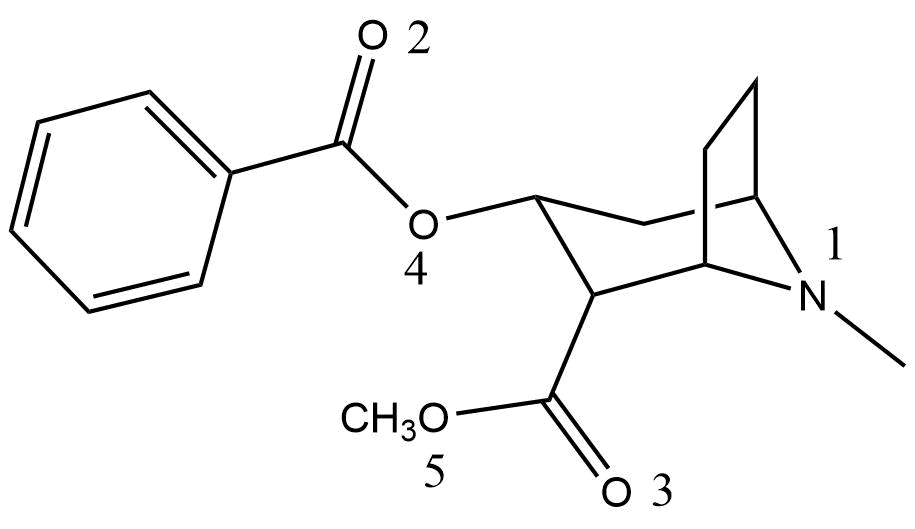
\includegraphics[width=\linewidth]{pics/cocaine-chapter/COC_struct.png}\end{minipage}\\ \midrule
Methyl ecgonine & 199 & 4.9$\times$10$^{-5}$& C$_{10}$H$_{17}$NO$_3$ & \begin{minipage}[c]{0.26\linewidth}\centering 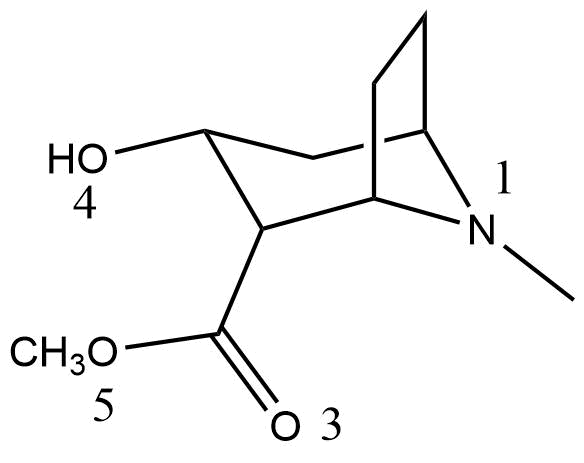
\includegraphics[width=.8\linewidth]{pics/cocaine-chapter/MeEcg_struct.png} \end{minipage} \\ \midrule
Cocaethylene & 317   &1.0$\times$10$^{-6}$ &  C$_{18}$H$_{23}$NO$_4$ & \begin{minipage}[c]{0.26\linewidth}\centering 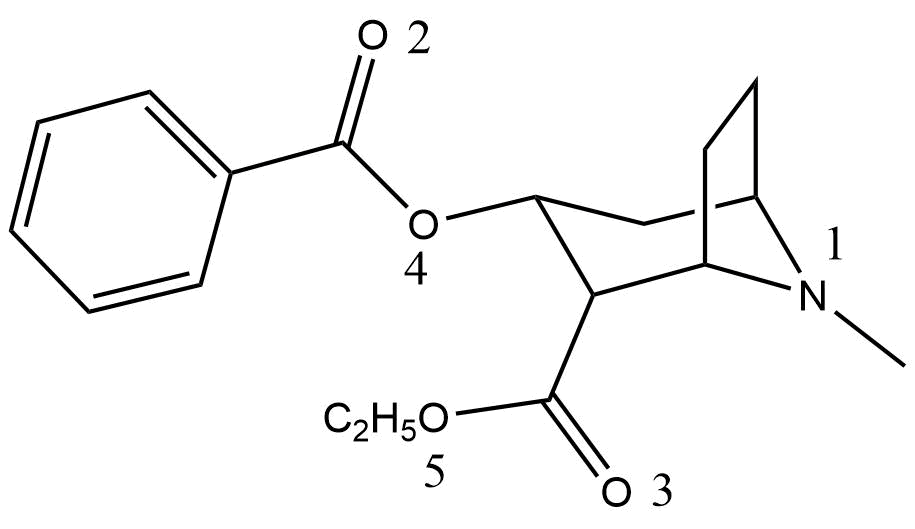
\includegraphics[width=\linewidth]{pics/cocaine-chapter/cocaet_struct.png} \end{minipage} \\ \midrule
Ethyl ecgonine & 213 & 7.8$\times$10$^{-6}$ &C$_{11}$H$_{19}$NO$_3$ & \begin{minipage}[c]{0.26\linewidth}\centering 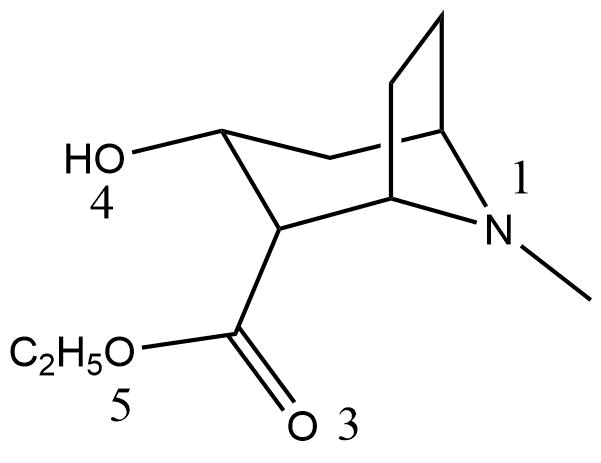
\includegraphics[width=.8\linewidth]{pics/cocaine-chapter/EtEcg_struct.png} \end{minipage} \\ \midrule
Norcocaine & 289 & - &C$_{16}$H$_{19}$NO$_4$ & \begin{minipage}[c]{0.26\linewidth}\centering 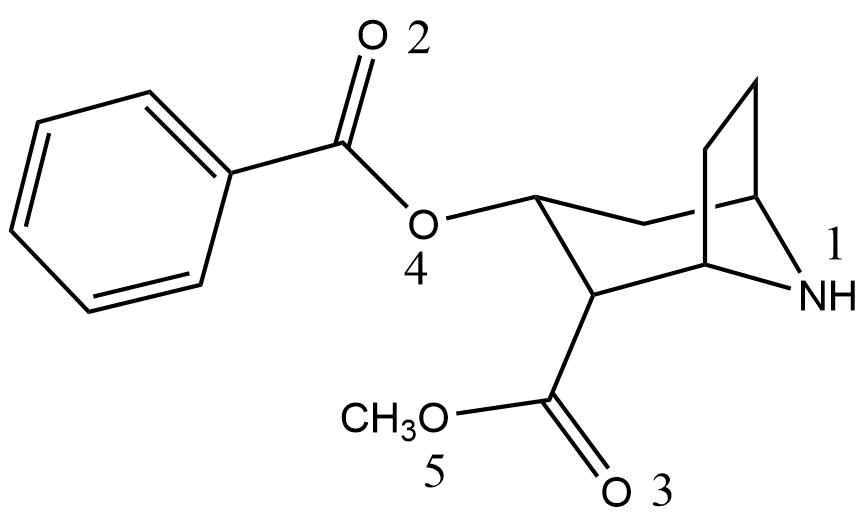
\includegraphics[width=\linewidth]{pics/cocaine-chapter/norcocaine_struct.png} \end{minipage}  \\ \midrule
Methyl ecgonidine & 181& 1.3$\times$10$^{-2}$ & C$_{10}$H$_{15}$NO$_2$ & \begin{minipage}[c]{0.26\linewidth}\centering 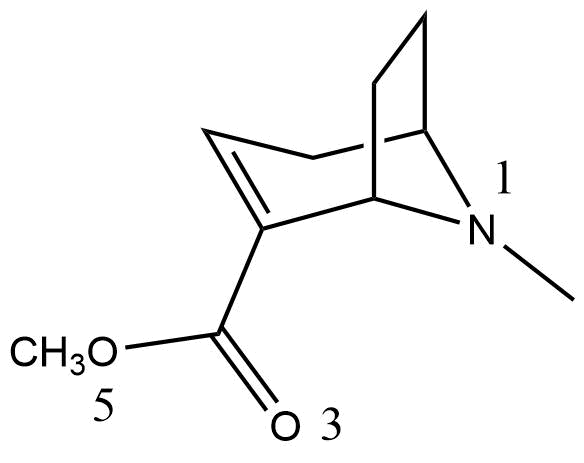
\includegraphics[width=0.8\linewidth]{pics/cocaine-chapter/ame_struct.png} \end{minipage}  \\ \midrule
o-Hydroxycocaine & 319 & - &C$_{17}$H$_{21}$NO$_5$ &  \begin{minipage}[c]{0.26\linewidth}\centering 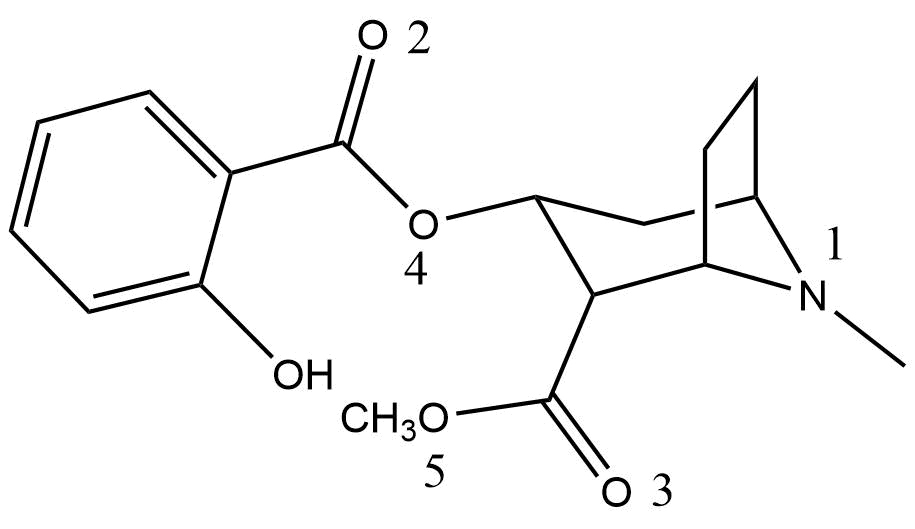
\includegraphics[width=\linewidth]{pics/cocaine-chapter/ohcocaine_struct.png} \end{minipage} \\ 
\bottomrule
\end{tabular}
\label{tab:structs}
\end{table}

\begin{table}
\centering
\caption{Nominal molecular weight, vapour pressure at 25$^\circ$C, formula and structure of benzoic acid, methyl benzoate, ethyl benzoate, isopropyl benzoate, methyl isobutyrate and ethyl isobutyrate.}
\begin{tabular}{lcccc}
\textbf{Compound} &  \textbf{MW} & \textbf{VP (mbar)} & \textbf{Formula} & \textbf{Structure} \\ 
\toprule
Benzoic acid &   122 &9.3$\times$10$^{-4}$&   C$_{7}$H$_{6}$O$_2$ & \begin{minipage}[c]{0.085\linewidth}\centering 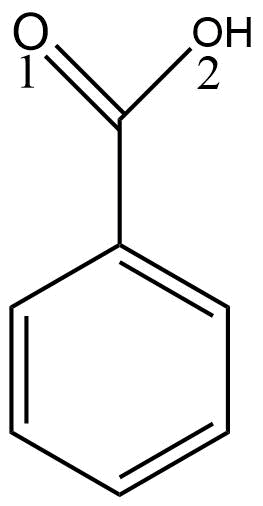
\includegraphics[width=\linewidth]{pics/cocaine-chapter/bzacid_struct.png}\end{minipage}\\ 
\midrule
Methyl benzoate &   136 &0.51&  C$_{8}$H$_{8}$O$_2$ & \begin{minipage}[c]{0.085\linewidth}\centering 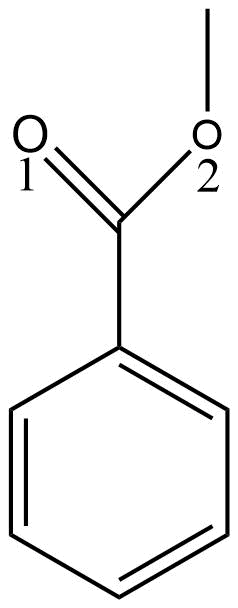
\includegraphics[width=\linewidth]{pics/cocaine-chapter/MeBz_struct.png}\end{minipage}\\ 
\midrule
Ethyl benzoate &   150 &0.36&   C$_{9}$H$_{10}$O$_2$ & \begin{minipage}[c]{0.105\linewidth}\centering 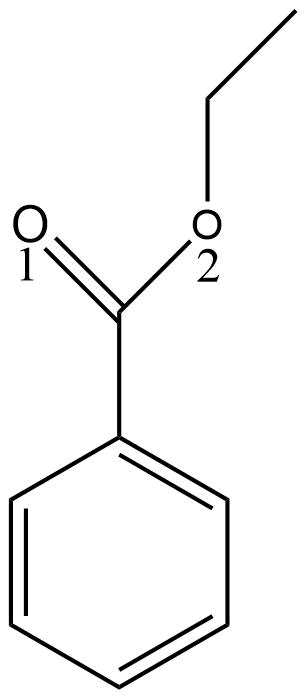
\includegraphics[width=\linewidth]{pics/cocaine-chapter/EtBz_struct.png}\end{minipage}\\ 
\midrule
Isopropyl benzoate &   164 &4.6$\times$10$^{-4}$&   C$_{10}$H$_{12}$O$_2$ & \begin{minipage}[c]{0.105\linewidth}\centering 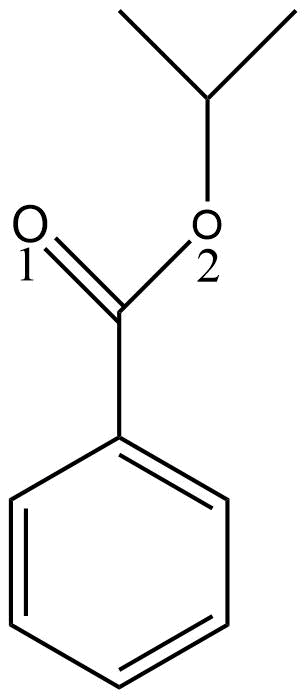
\includegraphics[width=\linewidth]{pics/cocaine-chapter/iPrBz_struct.png}\end{minipage}\\ 
\midrule
Methyl isobutyrate &   102 &65.7&   C$_{5}$H$_{10}$O$_2$ & \begin{minipage}[c]{0.13\linewidth}\centering 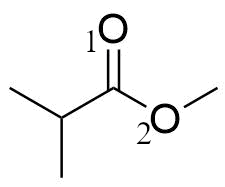
\includegraphics[width=0.8\linewidth]{pics/cocaine-chapter/MEisobuty_struct.png}\end{minipage}\\ 
\midrule
Ethyl isobutyrate &  116 &33.9&   C$_{6}$H$_{12}$O$_2$ & \begin{minipage}[c]{0.17\linewidth}\centering 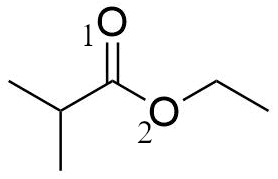
\includegraphics[width=0.8\linewidth]{pics/cocaine-chapter/ETisobuty_struct.png}\end{minipage} \\
\bottomrule
\end{tabular}
\label{tab:structs2}
\end{table}



\subsection{Reagent ions}\label{section:coc_RI}
For many of the compounds discussed in this chapter, a "normal" and humid \textit{E/N} study was done. The reagent ion signal for hydronium and the corresponding water cluster for these two sets of data are shown in \autoref{fig:RI_coc}. The abundance of the different water cluster species (i.e. (H$_2$O)$_n$H$_3$O$^+$) as a function of the reduced electric field that is observed in these figures are in agreement with those reported by \citeauthor{price1977new} as a function of the  reactor pressure, temperature and the \textit{E/P} ratio \cite{price1977new}.


A higher humidity in the drift tube can be achieved by increasing the humidity in the buffer gas, like \citeauthor{malaskova2019compendium} did \cite{malaskova2019compendium}. However, the measurements at higher humidity were unintended in my case, as the standard parameters setting (i.e. drift tube at 1 mbar and hollow cathode at 1.3 - 1.4 mbar)  yield such amount of water cluster ions that H$_3$O$^+$ is only more abundant than  (H$_2$O)H$_3$O$^+$ at reduced electric field values of 150 Td or more (\autoref{fig:RI_coc}b), which is occurring because the (H$_2$O)$_n$H$_3$O$^+$ ions don not break up prior their injection to the drift tube. This was found after doing a whole set of experiments in these humid conditions.
%
 Nevertheless, with the proton transfer from (H$_2$O)H$_3$O$^+$ being softer than that from H$_3$O$^+$, it is also necessary to acquire data in the driest conditions that the instrument could achieve to compare that data with the humid set. 
 %
The main consequence of a high abundance of water cluster ions at low \textit{E/N} is that it gets more complicated to ascertain whether the formation of a product ion at high \textit{E/N} is due to the higher collisional energy supplied by the electric field or is a consequence of the remaining energy after a harder proton transfer as the proton donating species is different than that at low \textit{E/N}.

The hollow cathode pressure can be reduced to minimise the clustering of reagent ions.
  However, there are two limitations when reducing the hollow cathode pressure: (i) lower pressure difference between cathode and drift tube increase the back-streaming of buffer gas  into the hollow cathode, generating undesirable reagent ions, and also (ii) at lower cathode pressures the instrument power boxes struggle to maintain the glow (i.e. the glow discharge indicator is flickering). 
%
A compromise was found at a hollow cathode pressure of 1.1 mbar and this drier configuration, whose reagent ion signal is shown in \autoref{fig:RI_coc}a, is referred to as "normal" conditions in this chapter.
%

The total reagent ion signal for each of the plots in \autoref{fig:RI_coc} present a maximum  at different values of the reduced electric field. This is correlated by the product ion plots provided in this chapter, which are given in raw counts per second to avoid the possible misleading effects created by normalising by the reagent ion signal or by calculating the branching percentages.
%
However, the raw cps do not give a quantitative measure on the abundance of ions  either, as the transmission of the ions along the different stages of the instrument depends on both the \textit{E/N} and the \textit{m/z} , but those are best quantity to use when comparing the findings from different instruments.

\begin{figure}[htbp]
\centering
\sidesubfloat[]{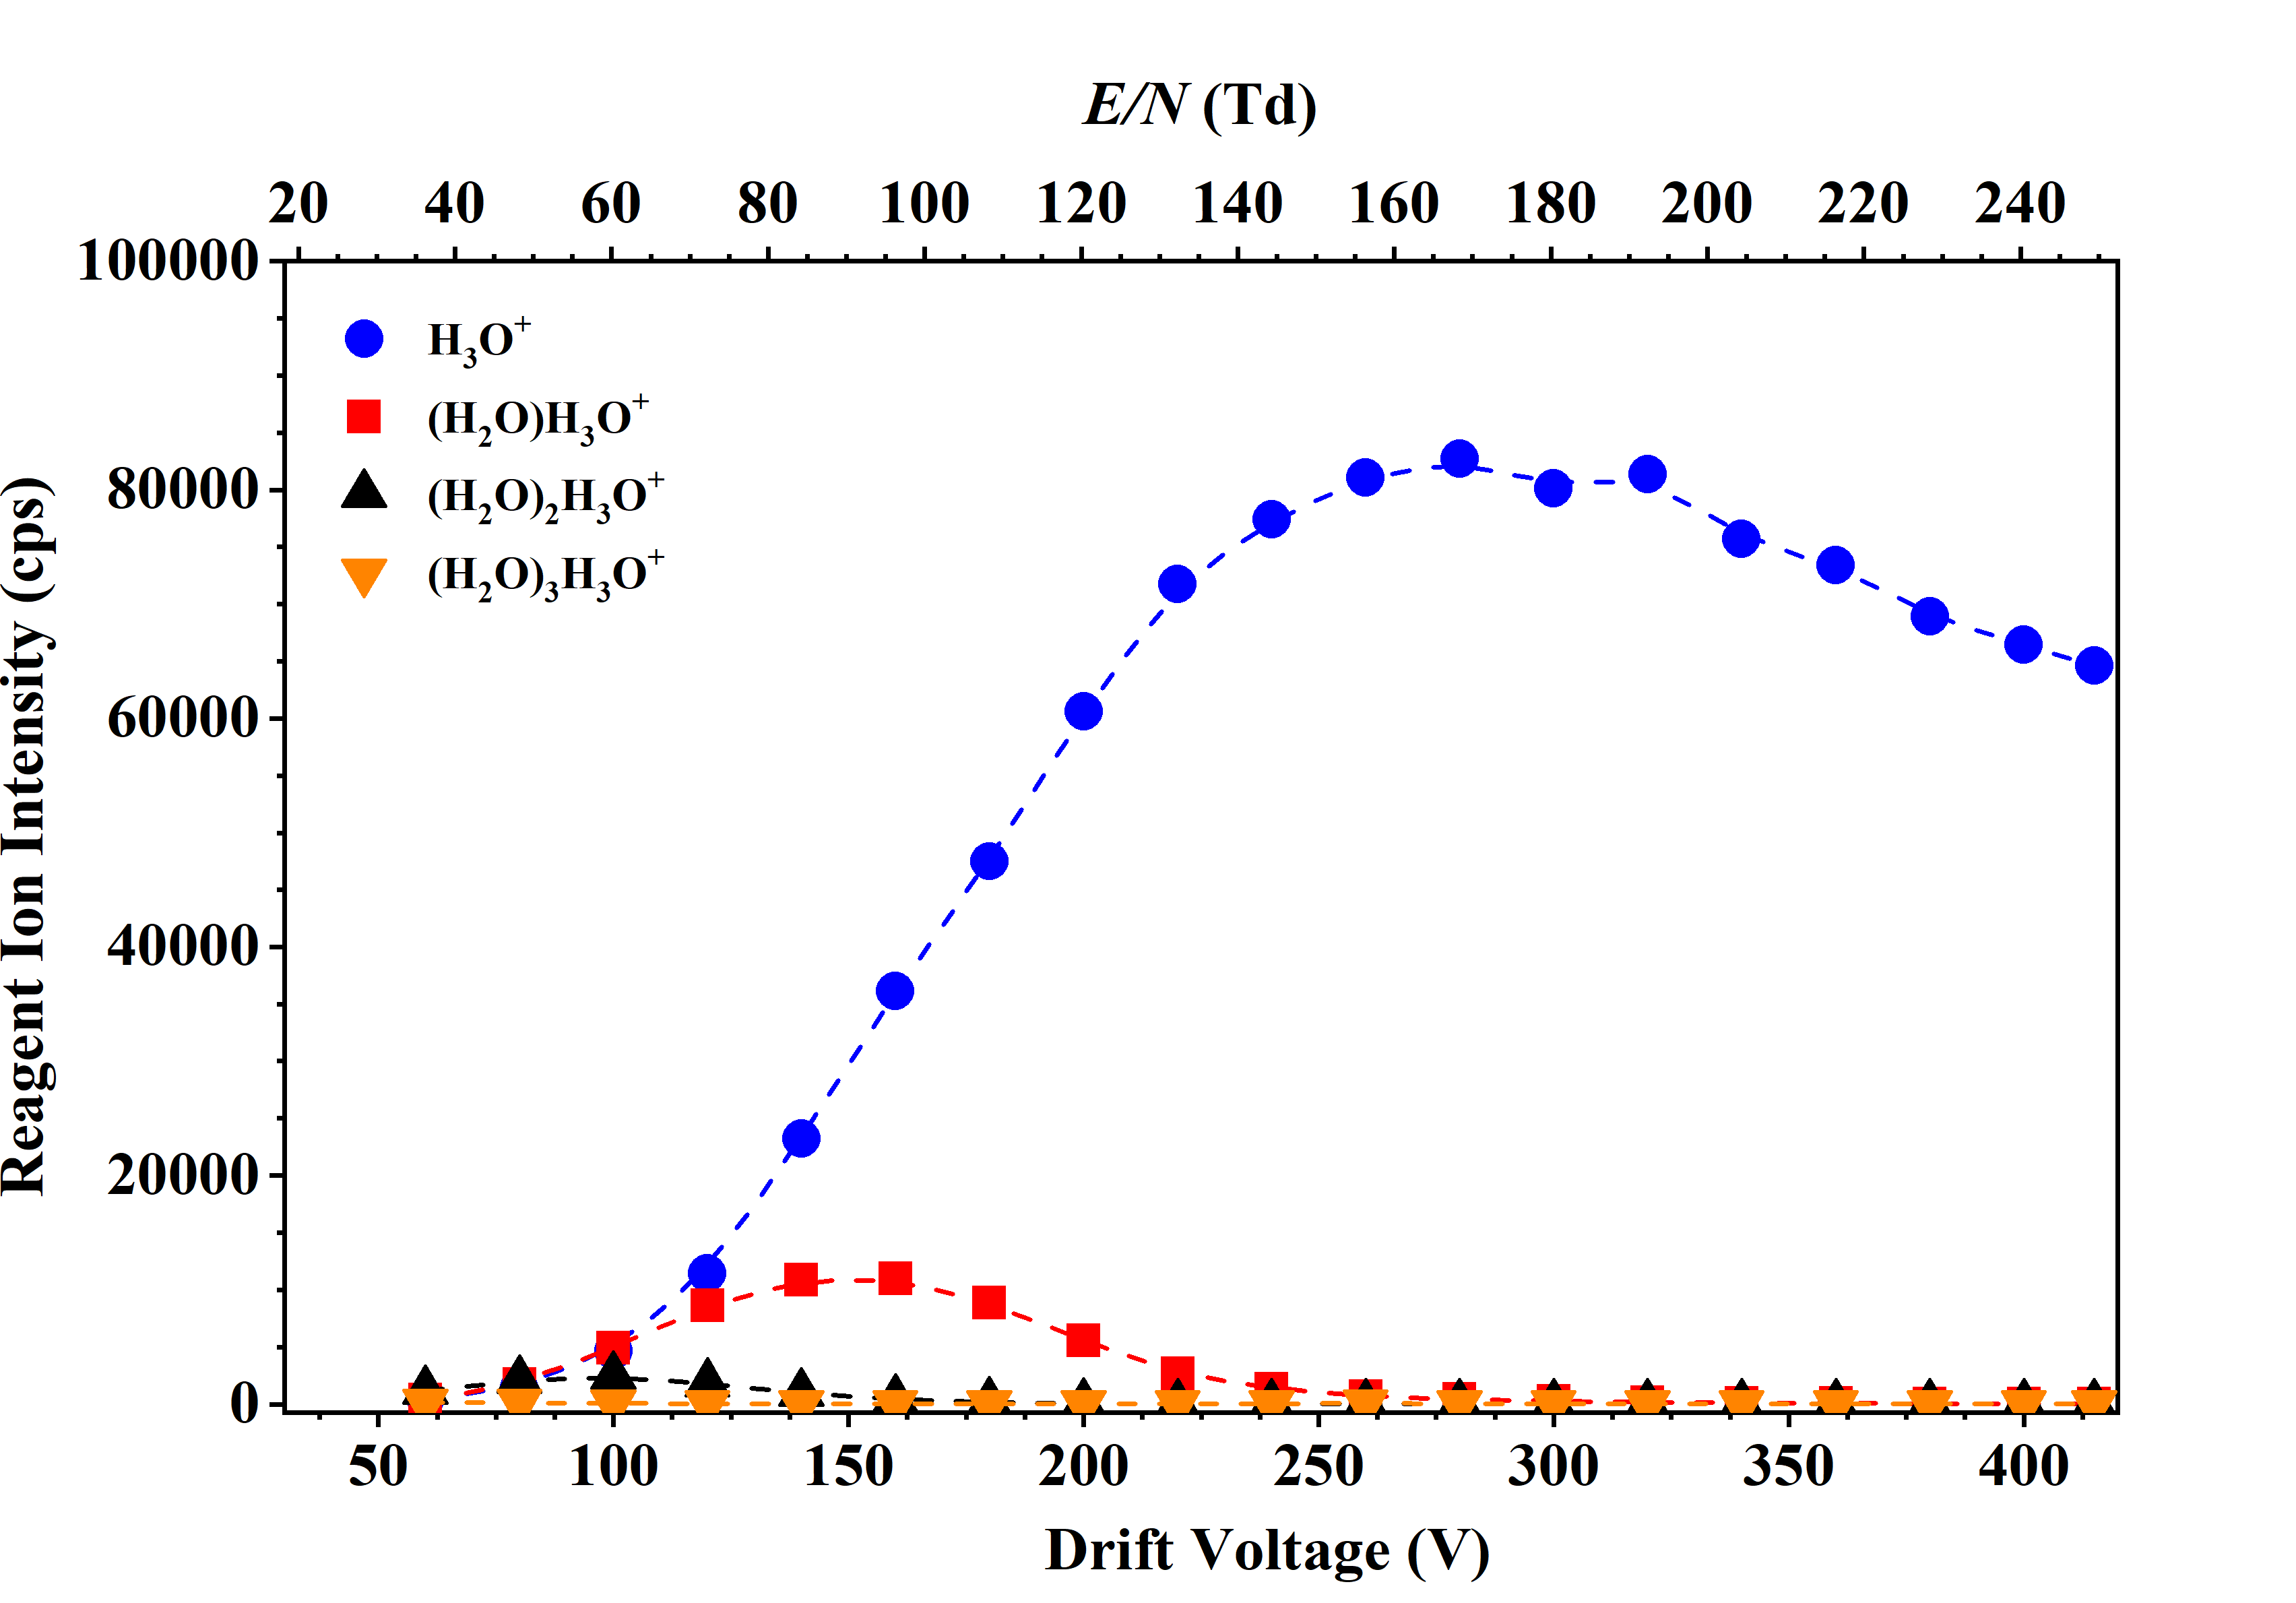
\includegraphics[width=0.8\linewidth]{pics/cocaine-chapter/RI.png}\label{fig:RI_coc_dry}}\\
\sidesubfloat[]{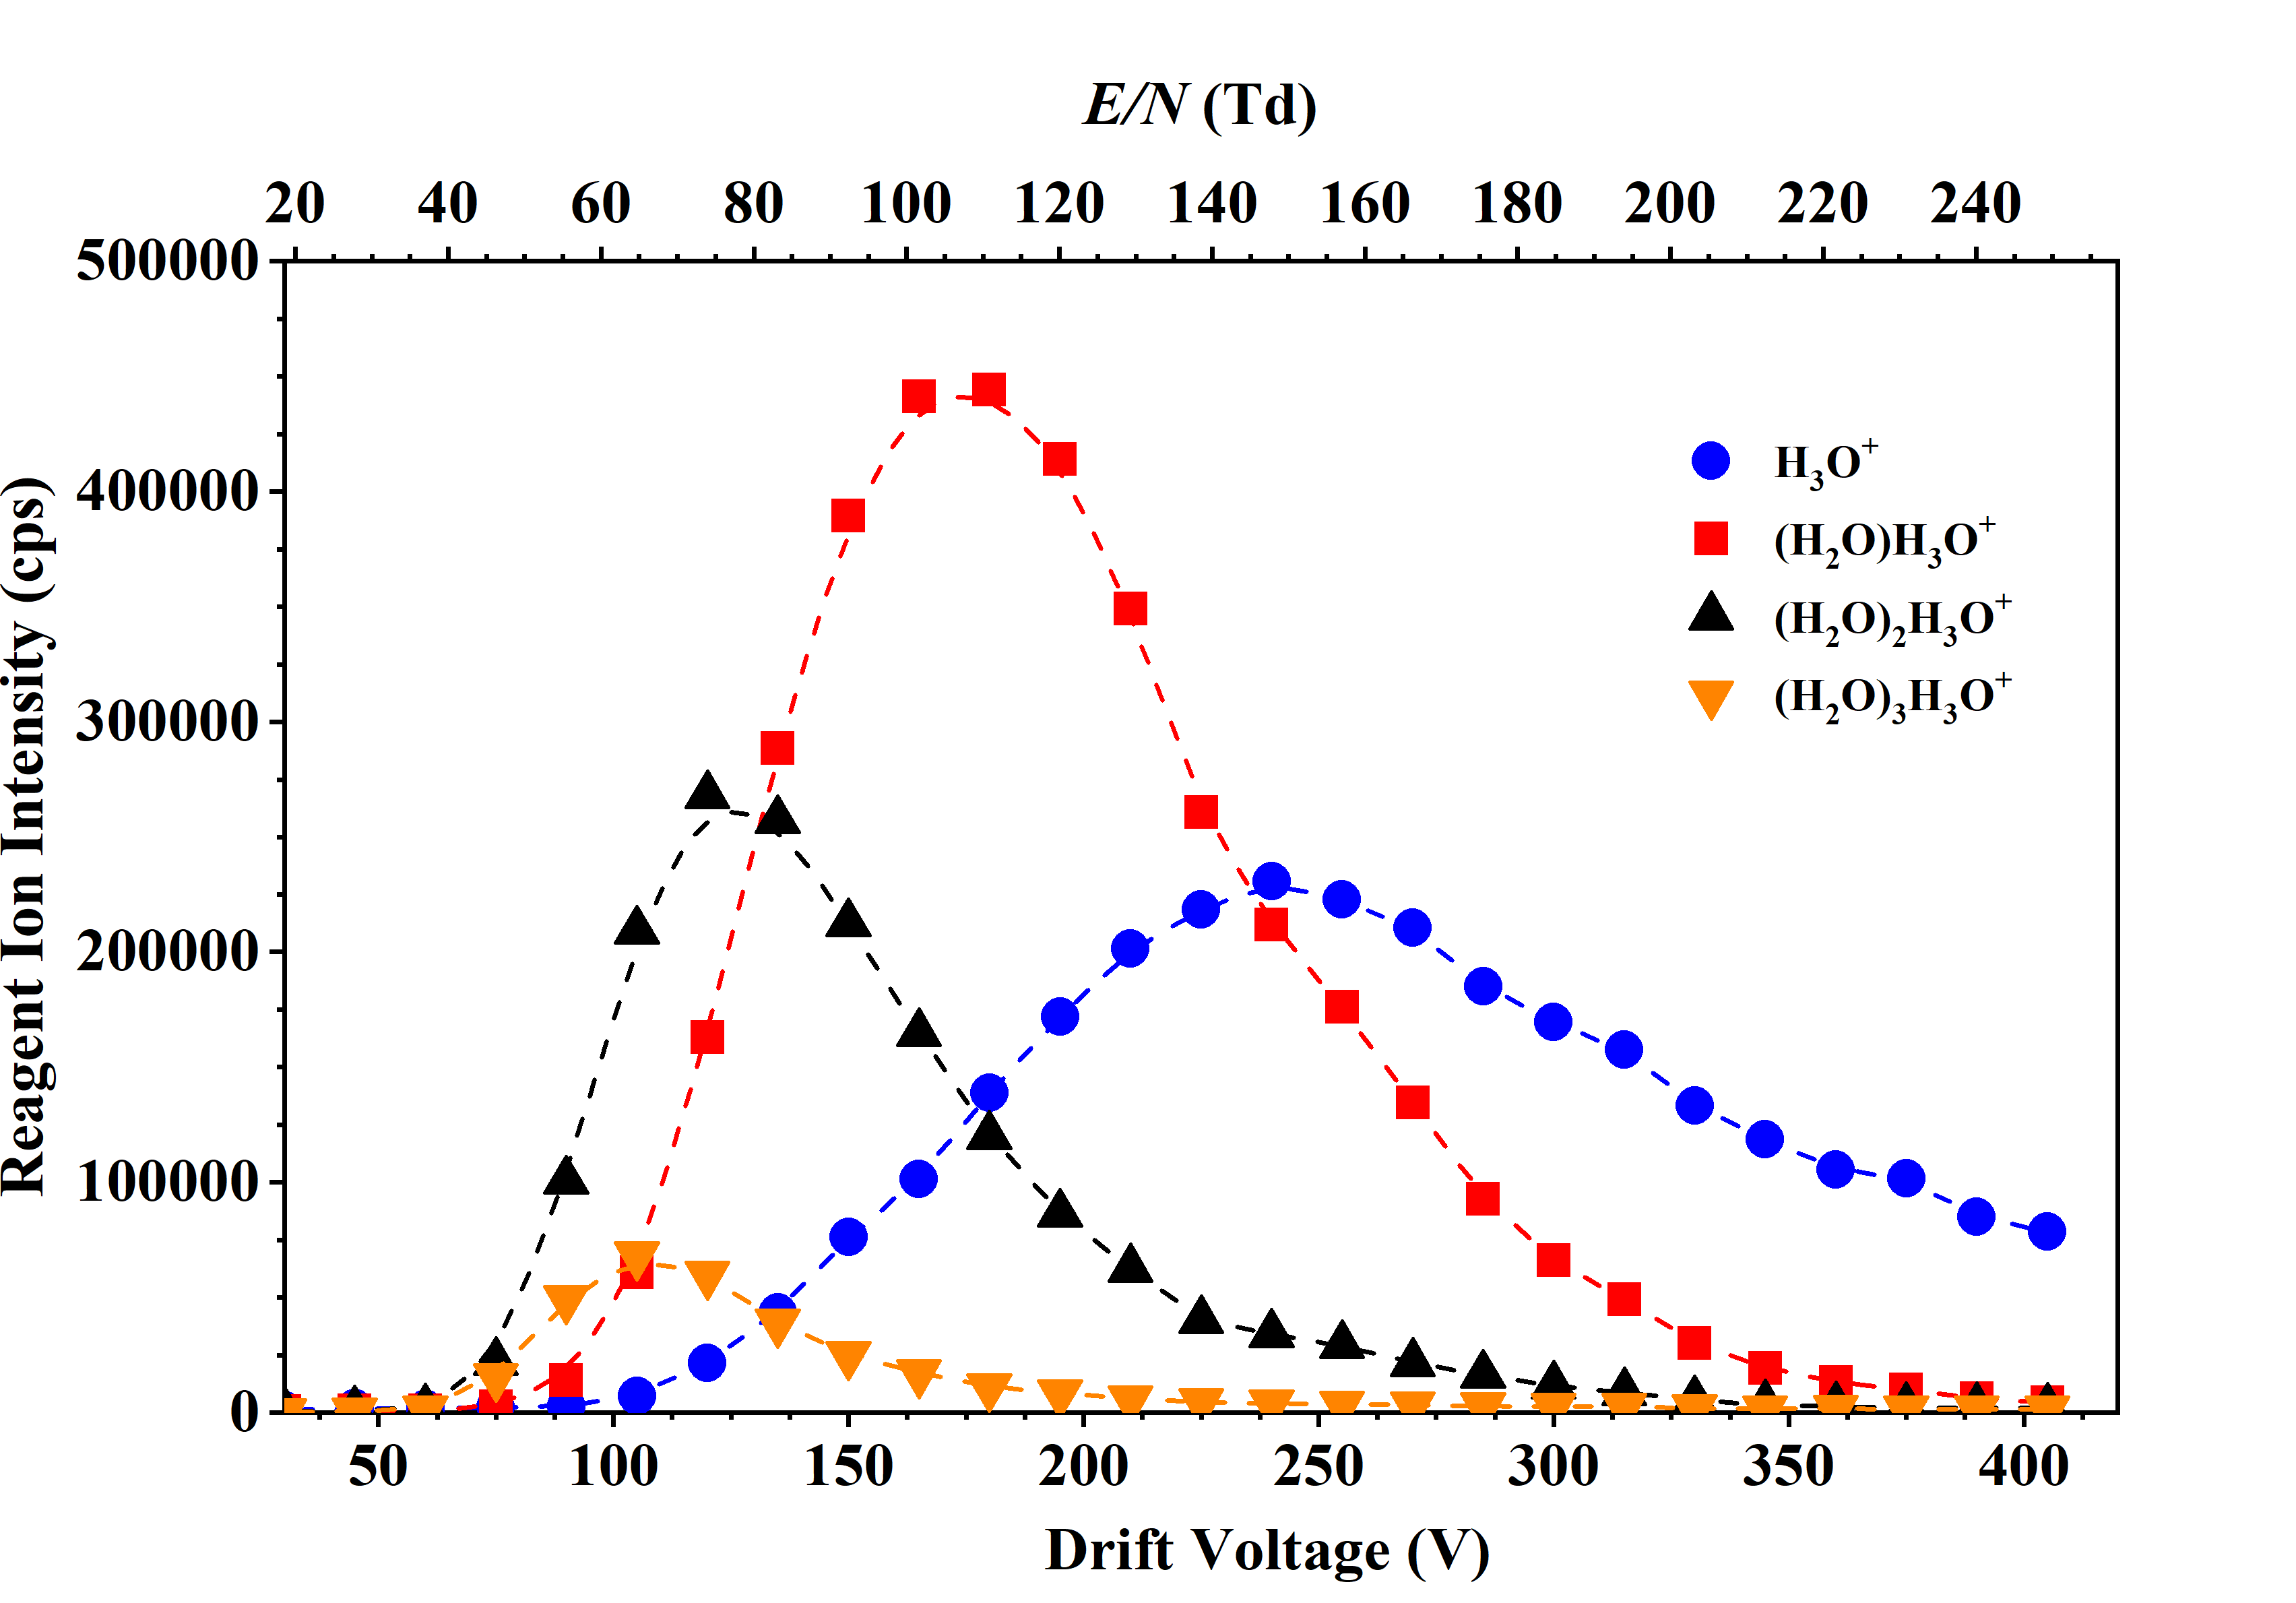
\includegraphics[width=0.8\linewidth]{pics/cocaine-chapter/humid/ri.png}\label{fig:RI_coc_humid}}
\caption{Reagent ion intensities in counts per second as a function of the drift voltage and the reduced electric field in (a) normal and (b) humid conditions.}
\label{fig:RI_coc}
\end{figure}

 
\subsection{Cocaine}
The structure of cocaine is given in \autoref{tab:structs}. The main protonation sites are the pyrolidine nitrogen N1, the benzoyl oxygen O2, the carbonyl oxygen O3, and the ester oxygen atoms O4 and O5.
%
DFT calculations show that the most basic site is N1 and the most stable structure of the protonated cocaine molecule is with the proton on N1 hydrogen bonded to O3. This structure is designated cocaine1H$^+$.
%
Likewise, when the proton is on O2 or O3 the structure is named cocaine2H$^+$ or cocaine3H$^+$.
%
Direct protonation of the ester sites O4 and O5 is possible.
%
The proton was found to be able to move between the studied basic sites and hence it will reside in the most basic site (N1).
In other words, MH$^+$ will predominantly be cocaine1H$^+$.
%
The displacement of the proton  from N1 to other sites  will result in fragmentation.
%
The PA and GB for the two most stable protonation sites of cocaine, N1 and O2, are given in \autoref{tb:co1} and these indicate that cocaine can be protonated from (H$_2$O)$_n$H$_3$O$^+$ up to n = 3.
Proton transfer from (H$_2$O)$_3$H$_3$O$^+$ would be actually thermoneutral as PA((H$_2$O)$_4$) = 1013 kJ mol$^{-1}$. 

\begin{table}[htbp]
\centering
\caption{Proton affinity and Gibbs free energy of the two most stable protonation sites of cocaine to yield the structures cocaine1H$^+$ and cocaine2H$^+$.}
\label{tb:co1}
\begin{tabular}{lcc}
\toprule
\textbf{Structure} &\textbf{PA (kJ/mol)} &\textbf{GB (kJ/mol)}\\ \toprule
Cocaine1H$^+$  & 1013 &   980    \\
Cocaine2H$^+$  & 933 &   895    \\
\bottomrule
\end{tabular}
\end{table}




The product ion intensities in cps for the reaction of (H$_2$O)$_n$H$_3$O$^+$ (n = 0, 1, 2, 3)  with cocaine are plotted in \autoref{fig:cocaineEN}.
%
These agree with the product ions reported in the literature \cite{Agarwal2011,wang1998collision}.
%
The dominant ion in both the normal and humid measurements is the protonated parent molecule MH$^+$ (i.e. (C$_{17}$H$_{21}$NO$_4$)H$^+$) from non-dissociative proton transfer. 
%
There are other product ions observed with less abundance.
%
The ion at \textit{m/z} 182 (i.e. C$_{10}$H$_{16}$NO$_2^+$) is a carbocation resulting from the loss of benzoic acid from MH$^+$, while the one at \textit{m/z} 272 (i.e. C$_{16}$H$_{18}$NO$_3^+$) is an acyl following the loss of methanol (MeOH) from  MH$^+$.
%
At high \textit{E/N}, C$_{5}$H$_{8}$N$^+$ is found at \textit{m/z} 82.
%
In humid conditions two other ions are also observed: benzoyl$^+$ at \textit{m/z} 105 and protonated benzoic acid at \textit{m/z} 123.
%



 
\begin{figure}[htbp]
\centering
\sidesubfloat[]{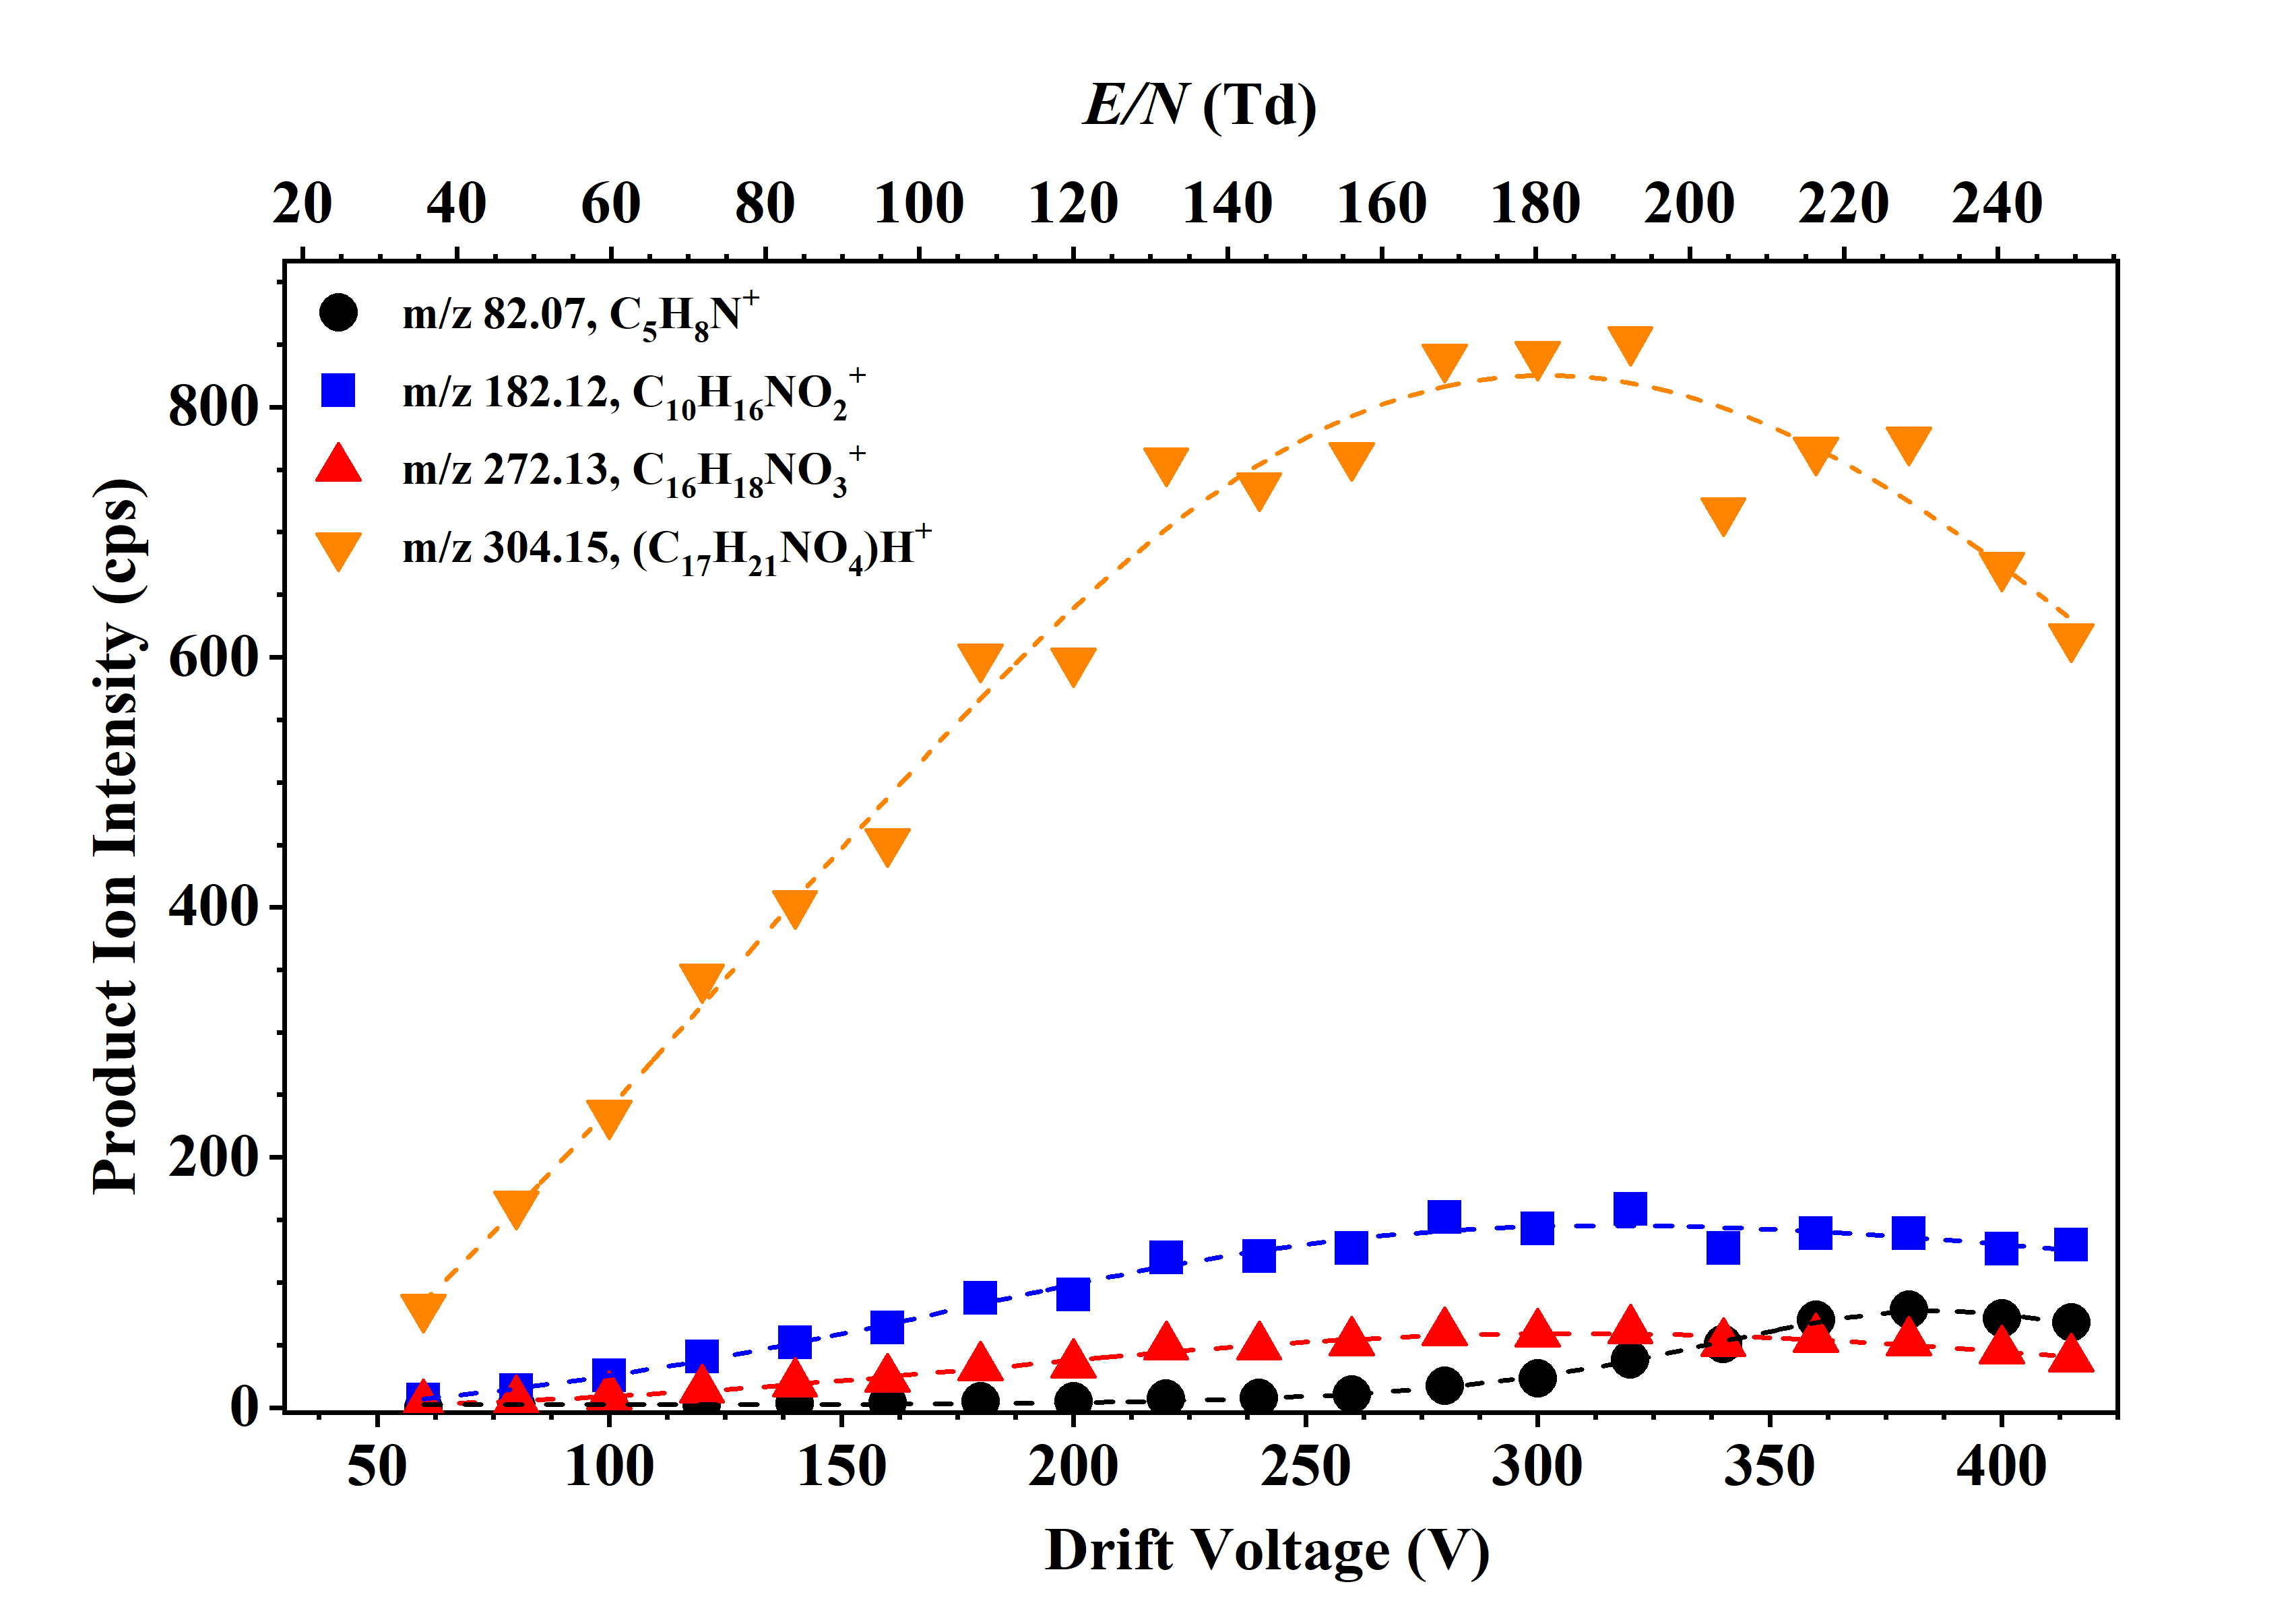
\includegraphics[width=0.8\linewidth]{pics/cocaine-chapter/COC-CPS.png}}\\
\sidesubfloat[]{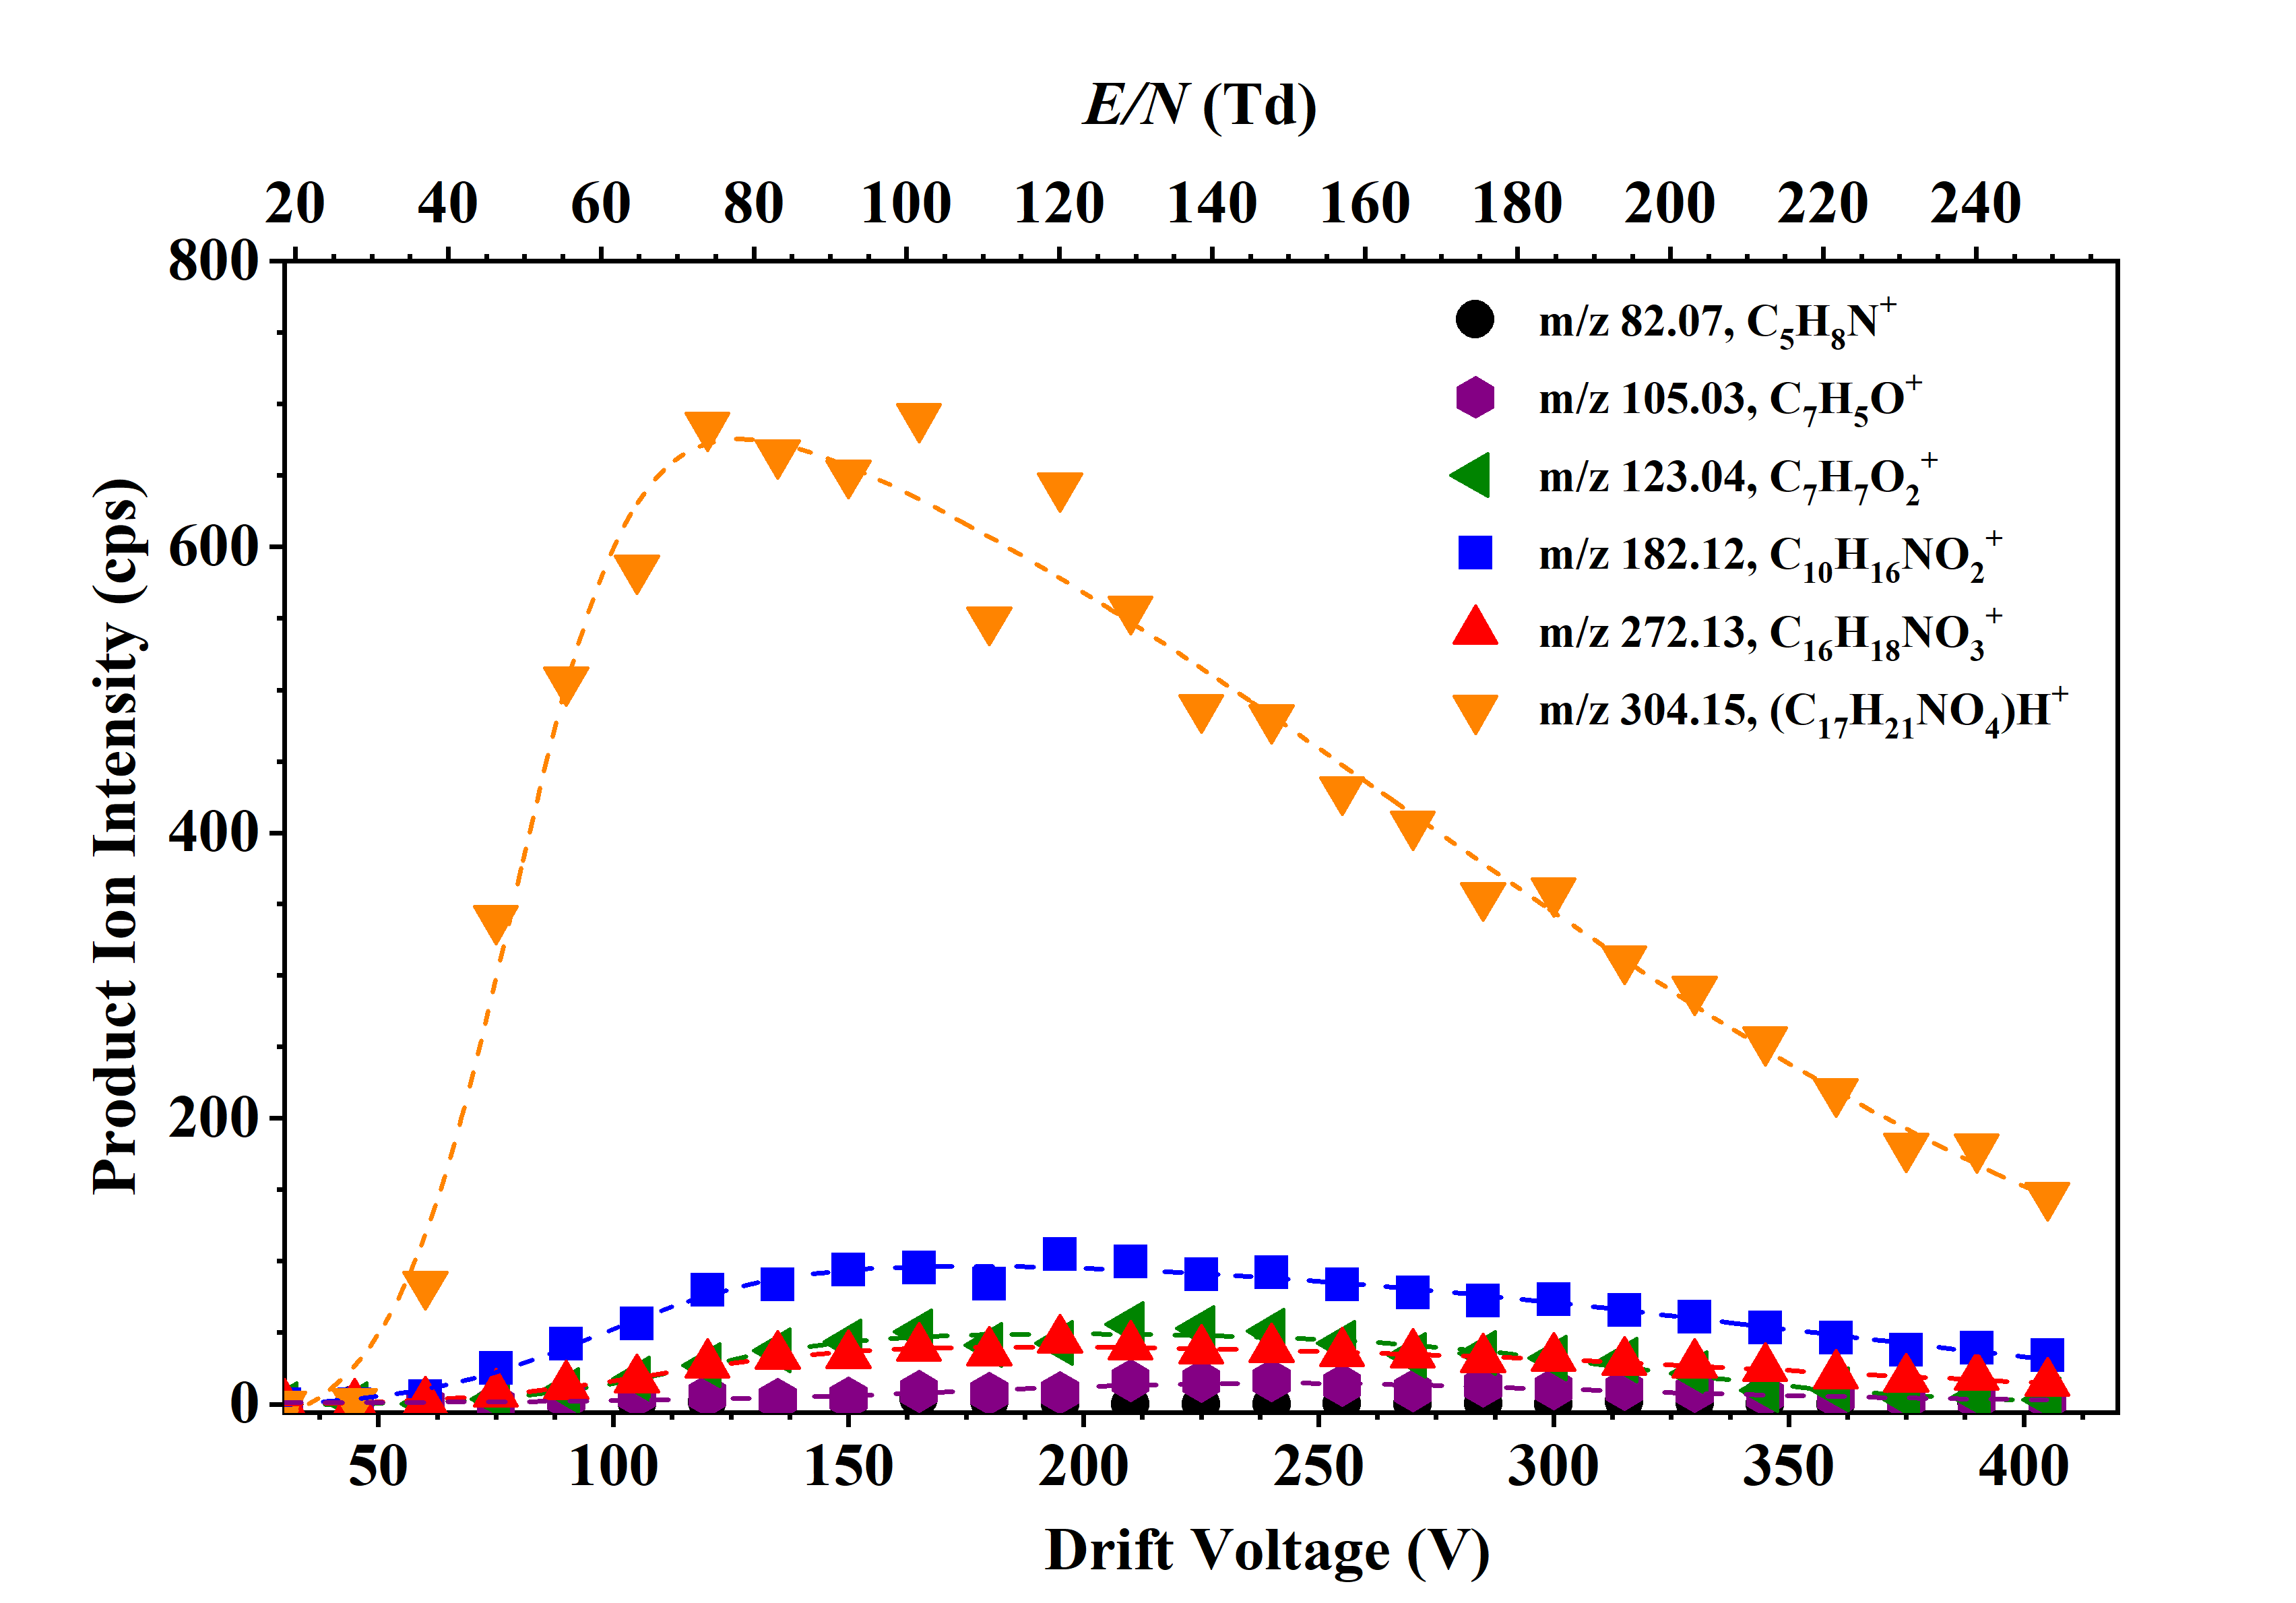
\includegraphics[width=0.8\linewidth]{pics/cocaine-chapter/humid/cocaine-cps.png}}
\caption{Product ion signal intensities in counts per second of the product ions resulting from reactions of the H$_3$O$^+$.(H$_2$O)$_n$ (n = 0, 1, 2, 3) with cocaine as a function of the drift voltage and the reduced electric field in (a) normal and (b) humid conditions}
\label{fig:cocaineEN}
\end{figure}

The energetics associated to the formation of the studied product ions are given in \autoref{tb:co2}. 
%
These are only compared to H$_3$O$^+$ and (H$_2$O)H$_3$O$^+$ because these are the most relevant reagent ions: they are the most abundant in the 100 - 200 Td range and also proton transfer from (H$_2$O)$_2$H$_3$O$^+$ or (H$_2$O)$_3$H$_3$O$^+$ would be similar to that from (H$_2$O)H$_3$O$^+$.
%
Even with all the fragmentation pathways being thermodynamically allowed, it is surprising that MH$^+$ is the dominant ion for all the \textit{E/N} range.
%
One could think that in the humid results most of the MH$^+$ ion comes from the reaction with the water clusters (i.e. (H$_2$O)H$_3$O$^+$ and (H$_2$O)$_2$H$_3$O$^+$), but as similar proportions of product ions are observed in the normal case, this cannot be the reason.
%
It is more likely that the proton stays in the the most basic site (i.e. N1) and its transfer to other sites, which is thermodynamically allowed and needed for fragmentation to occur, does not occur fast.
%
%
%In the next paragraphs the formation process of the main product ions is discussed.


The formation of the ion at \textit{m/z} 272 is the result of the loss of MeOH in the methyl ester moiety of the protonated cocaine molecule.
%
This happen through a barrierless dissociation when the proton is in O5. 
%
The migration from the protonation site to O5 occurs through a transition state.
%
Two transition states were found, named TS2 and TS2A.
%
TS2 refers to the transfer of the proton from the more basic carbonyl oxygen O3 to the less basic ester oxygen O5 followed by the split up of the C--O5 bond.
%
TS2A is similar to TS2 with the proton migrating from the benzoyl oxygen O2 instead. %to the ester oxygen O5.
%
TS2 is marginally exergonic (i.e. -9 kJ mol$^{-1}$ for the reaction with H$_3$O$^+$) while TS2A has much lower energy requirements (i.e. -111 kJ mol$^{-1}$ for the reaction with H$_3$O$^+$).
%
Furthermore, the abundance of the ion at \textit{m/z} 272 is comparable to other fragment ions, which hints that the formation of this ion is carried out through the transition state TS2A.


%    Normally loss of MeOH from a methyl ester is relatively straightforward. The transition state is the migration of the proton from the more basic carbonyl oxygen (O3) to the less basic ester oxygen (O5) with the concomitant breaking of the C – O5 bond and barrierless dissociation of MeOH. This transition state will be designated TS2. However, a similar transition state involving the migration of a proton from the benzoyl oxygen O2 to O5 has been found and is designated TS2A. This is considerably lower in energy than TS2. Whilst TS2 is slightly exergonic and is thus an accessible pathway the similarity in in yield to the other fragmentation pathways suggests that the fragmentation involving TS2A is operative. 
    %
\begin{table}[htbp]
\centering
\caption{Energetics of the reaction of cocaine with (H$_2$O)$_n$H$_3$O$^+$ (n = 0, 1) yielding the respective structure or transition state. $\Delta$H$_{298}$ and $\Delta$G$_{298}$ are relative to cocaine and H$_3$O$^+$ and, in brackets, to cocaine and (H$_2$O)H$_3$O$^+$.}
\label{tb:co2}
\begin{tabular}{lccc}
\toprule
\textbf{Reaction or transition state}	&\textbf{\textit{m/z} } &\textbf{$\Delta$H$_{298}$} &\textbf{$\Delta$G$_{298}$}\\
& &	\textbf{(kJ/mol)} &\textbf{(kJ/mol)} \\  \toprule
Cocaine1H$^+$  				&	304	& -328 (-170)  & -326 (-202)   \\ \midrule
(CocaineH$^+$ - MeOH) + MeOH   			&	272	& -138 (+20)	&-186 (-62)   \\ \midrule
(CocaineH - benzoic acid)$^+$ + benzoic acid &	182 & -272 (-114)  & -336 (-212)  \\ \midrule
(CocaineH - benzoyl) + benzoyl$^+$    	&	105	& -54 (+104)  & -104 (+20)  \\ \midrule
(Cocaine - benzoic acid) + benzoic acidH$^+$& 123	& -88 (+70)  & -144  (-20) \\ \midrule
MeOH loss: TS2 for H migration O3 to O5& & -8 (+150)  & -9 (+115)  \\ \midrule
MeOH loss: TS2A for H migration O2 to O5& & -119 (+39)  & -111  (+13) \\ 
\bottomrule
\end{tabular}
\end{table}


Possible structures for the C$_5$H$_8$N$^+$ product ion at \textit{m/z} 82 are provided in \autoref{fig:coc_82}. 
%
The nitrogen atom N1 is the most basic site of the cocaine molecule and hence the first structure was thought to be the correct one.
%
However, experiments from \citeauthor{wang1998collision} using deuterated precursor ions in a triple quadruple system also yield the product ion at \textit{m/z} 82, which proves that the deuterium (or proton in our case) is not part of this ion and therefore the right structure must be the second or the third of those in \autoref{fig:coc_82}, with the third structure being 16 kJ mol$^{-1}$ more stable than the second one \cite{wang1998collision}.
%
Furthermore, \citeauthor{wang1998collision} reported this ion in higher abundance than it was found in PTR-MS, and they also found the ion at \textit{m/z} 182 to be the dominant ion, rather than MH$^+$ as it is observed in PTR-MS. These differences can be explained in terms of the collisional energy. The range of energies used by \citeauthor{wang1998collision} was in the range 17 - 23 eV, while in PTR-MS the collisional energies are calculated to be ca. 1 eV and below (see \autoref{fig:KE}).
%
C$_5$H$_8$N$^+$ is also found in methyl ecgonine, cocaethylene and ethyl ecgonine but its formation will not be analysed for now because it is only found at a low abundance at high reduced electric fields and it is a product of field-activated collision-induced dissociation.




%The fragment ion with \textit{m/z} 82 was initially thought to have the first structure in \autoref{fig:coc_82} but experiments using D$_2$O in a Triple Quad by \citeauthor{wang1998collision} showed no inclusion of deuterium in the ion which must therefore have one of the other two structures, the final structure being marginally more stable by 16 kJ mol$^{-1}$ \cite{wang1998collision}. They also observed it in larger quantities than in the present work as did \citeauthor{clauwaert1998narrow}  \cite{clauwaert1998narrow}. It is also observed with MeEcg and other analogues of Cocaine but in such small amounts and high \textit{E/N} its formation will not be pursued further at present. It is interesting that whilst all fragmentation routes are energetically favourable (see later discussion for loss of Benzoic acid from protonated Benzoate esters) little fragmentation is observed. This could be ascribed to very little H$_3$O$^+$ being present and the dominance of MH$^+$ being due to reaction of Cocaine with \textit{m/z} 37 and \textit{m/z} 55. But since similar patterns of behaviour are observed under both wet and dry conditions whilst the mass spec of the reagent ions are very different for the two conditions (see reagent ions) this is most unlikely. A more plausible explanation is that the proton is sequestered on N1 and its migration to the fragmentation sites whilst thermodynamically feasible is very slow. 


\begin{figure}[htbp]
\centering
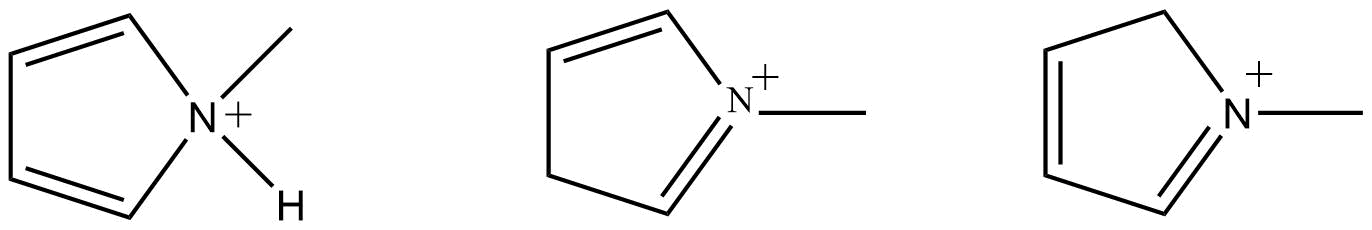
\includegraphics[width=0.6\linewidth]{pics/cocaine-chapter/mz82.png}
\caption{Possible structures of the fragment ion at \textit{m/z} 82 from the reaction of cocaine with (H$_2$O)$_n$H$_3$O$^+$. }
\label{fig:coc_82}
\end{figure}


The formation of C$_{10}$H$_{16}$NO$_2^+$ at \textit{m/z} 182 requires the elimination of benzoic acid from the protonated parent molecule.
%
This needs the proton to be on O2 or O4 during the transition state, after which the benzoic acid is removed (i.e. the C--O4 bond breaks), yielding protonated methyl ecgonidine (see \autoref{fig:coc_182}).
%
However, the fact that the transition state was not found and that two other ions coming from the benzoate moiety (i.e. \textit{m/z} 105 and \textit{m/z} 123) were seen only in the humid conditions drove this research to the examination of a cocaine homologue, methyl ecgonine, and a series of benzoate esters.

%    In order to eliminate Benzoic acid a proton will have to be present on either O2 or O4 during the transition state. Unfortunately, attempts to find a transition state were unsuccessful with the proton migrating to O3.  Irrespective of whether the proton is on O2 or O4 when the benzoic acid departs the resulting carbocation will have the structure shown in  \autoref{fig:coc_182}, which is a protonated methyl ecgonidine.
%
%Because of the unsuccessful search for a TS for the loss of benzoic acid to give \textit{m/z} 182 and the observation of two other ions arising from the benzoate moiety viz. \textit{m/z} 123 and \textit{m/z} 105 under wet conditions it was thought useful to examine a series of benzoate esters and related compounds.% before investigating an abbreviated homologue of cocaine, benzoyl ecgonine (BzEcg).
% Before that is was considered interesting to investigate another abbreviated homologue of cocaine, methyl ecgonine (MeEcg).
 
%At present we have no explanation as to why \textit{m/z} 105 and \textit{m/z} 123 are only seen under wet conditions.



%\begin{figure}[htbp]
%\centering
%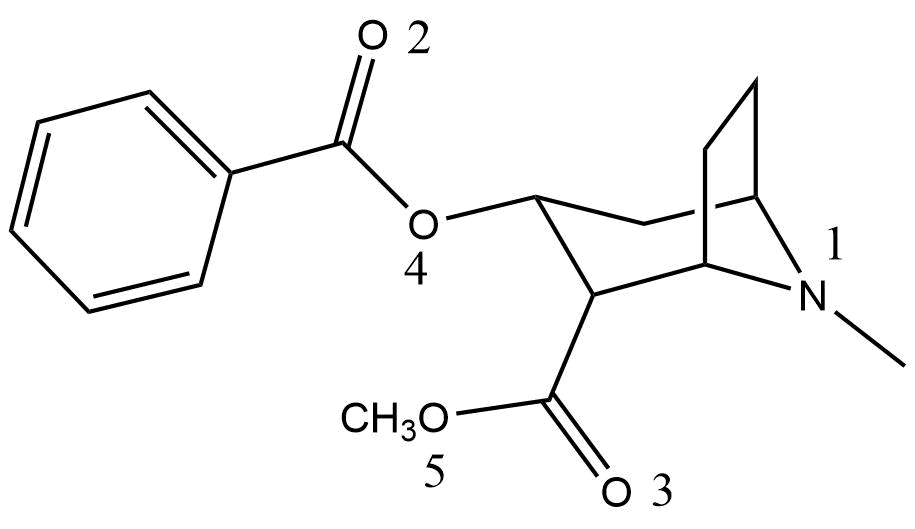
\includegraphics[width=0.4\linewidth]{pics/cocaine-chapter/COC_struct.png}
%\caption{Structure  of cocaine, including the numbering of the main protonation sites.}
%\label{fig:cocaine_struct}
%\end{figure}




\begin{figure}[htbp]
\centering
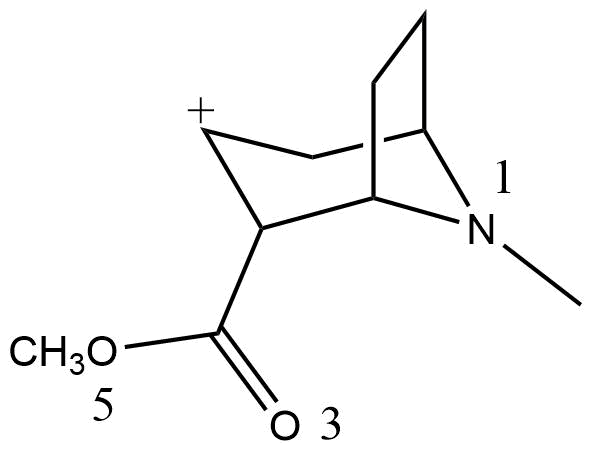
\includegraphics[width=0.25\linewidth]{pics/cocaine-chapter/coc_182.png}
\caption{Structure of the fragment ion at \textit{m/z} 182 from the reaction of cocaine with (H$_2$O)$_n$H$_3$O$^+$.}
\label{fig:coc_182}
\end{figure}



%\begin{figure}[htbp]
%\centering
%\scalebox{0.5}{
%\begin{tikzpicture}
%\chemfig{[:180]**6(------)-[::210](=[::60]O^2)-[::-60]O^4>[::75](?[a])-[::30]-[::-60,1.4](<:[::60]H)(-[::-60]N^1?[b,{-}]-[::15])-[::90,1.1]-[::135,0.8]-[::45,1.1](?[b])(<[::0]H)-[::-60]?[a](<[::45](=[::60]O^3)-[::-60]O^5-[::60])}
%%\chemfig{[:180]**6(------)-[::210](=[::60]O)-[::-60]O>[::75](?[a])-[::30]-[::-60,1.4](<:[::60]H)(-[::120]N?[b,{-}]-[::-15])-[::-30,1.1]-[::-90,0.8]-[::-90,1.1](?[b])(<[::105]H)-[::60]?[a](<[::45](=[::60]O)-[::-60]O-[::60])} %previous version with the N in opposite way
%\end{tikzpicture}
%}\label{fig:coc}
%\caption{Cocaine}
%\end{figure}



 
 

\subsection{Methyl ecgonine}
%Methyl ecgonine (MeEcg, C$_{10}$H$_{17}$NO$_3$) is the .........
%It is used as biomarker for crack (smoked cocaine) consumption.

The protonation sites for methyl ecgonine (MeEcg) are numbered in the same way as those for cocaine (see structure in \autoref{tab:structs}). 
%
The PA and GB of the protonation sites that give the two most stable structures of protonated methyl ecgonine are given in \autoref{tb:me1}.
%
MeEcg can undergo proton transfer from (H$_2$O)$_n$H$_3$O$^+$ for n = 0, 1 and 2, as PA((H$_2$O)$_3$) = 937 kJ mol$^{-1}$.
%
The structure MeEcg1H$^+$ is with the proton on the pyrolidine nitrogen (N1) hydrogen bonded to O3. 
%
MeEcg3H$^+$ is with the proton hydrogen between and hydrogen bonded to O3 and O4.
%
Similar to cocaine, the proton can move between the protonation sites although it will be mainly  on N1. 
%


    %As with cocaine, inspection of the various protonated structures shows that the proton is mobile and has no difficulty in moving between the various basic sites although as with Cocaine it will be primarily sequestered on N1. The energetics for the two most stable structures are given in \autoref{tb:me1}.
%
    %As with cocaine when the proton is on the pyrolidine nitrogen N1 it is hydrogen bonded to O3.  In MeEcg3H$^+$ the proton is hydrogen bonded between O4 and O3. The transition state for the loss of MeOH is migration of the proton from O3 to O5 followed by the barrierless dissociation of MeOH. The energetics are similar to those found for TS2 in cocaine. However direct protonation of O5 may occur. 

\begin{table}[htbp]
\centering
\caption{Proton affinity and Gibbs free energy of the two most stable protonation sites of methyl ecgonine that yield the structures MeEcg1H$^+$ and MeEcg3H$^+$.}
\label{tb:me1}
\begin{tabular}{lcc}
\toprule
\textbf{Structure} &\textbf{PA (kJ/mol)} &\textbf{GB (kJ/mol)}\\ \toprule
MeEcg1H$^+$  & 996 &   965    \\
MeEcg3H$^+$  & 906 &   873    \\
\bottomrule
\end{tabular}
\end{table}

\autoref{fig:MeEcgEN} shows the product ion intensities  for the reaction of  (H$_2$O)$_n$H$_3$O$^+$ (n = 0, 1, 2) with  methyl ecgonine as a function of the drift voltage and reduced electric field.
%
The difference in ion intensities between the normal and humid case can be explained in terms of the reagent ion intensities for each case (see \autoref{fig:RI_coc}).
%
The observed product ions follow similar fragmentation pathways as those found with cocaine.
%
The dominant ion in both the normal and humid case is MH$^+$.
%
Other found product ions are C$_{9}$H$_{14}$NO$_2^+$ at \textit{m/z} 168 or C$_{10}$H$_{16}$NO$_2^+$ at \textit{m/z} 182, resulting from the loss of MeOH or H$_2$O from the protonated parent molecule in each case.
%
Traces of C$_5$H$_8$N$^+$ at \textit{m/z} 82 are also found at high \textit{E/N} (>140 Td) but, as mentioned in the cocaine section, this will not be further investigated.

\begin{figure}[htbp]
\centering
\sidesubfloat[]{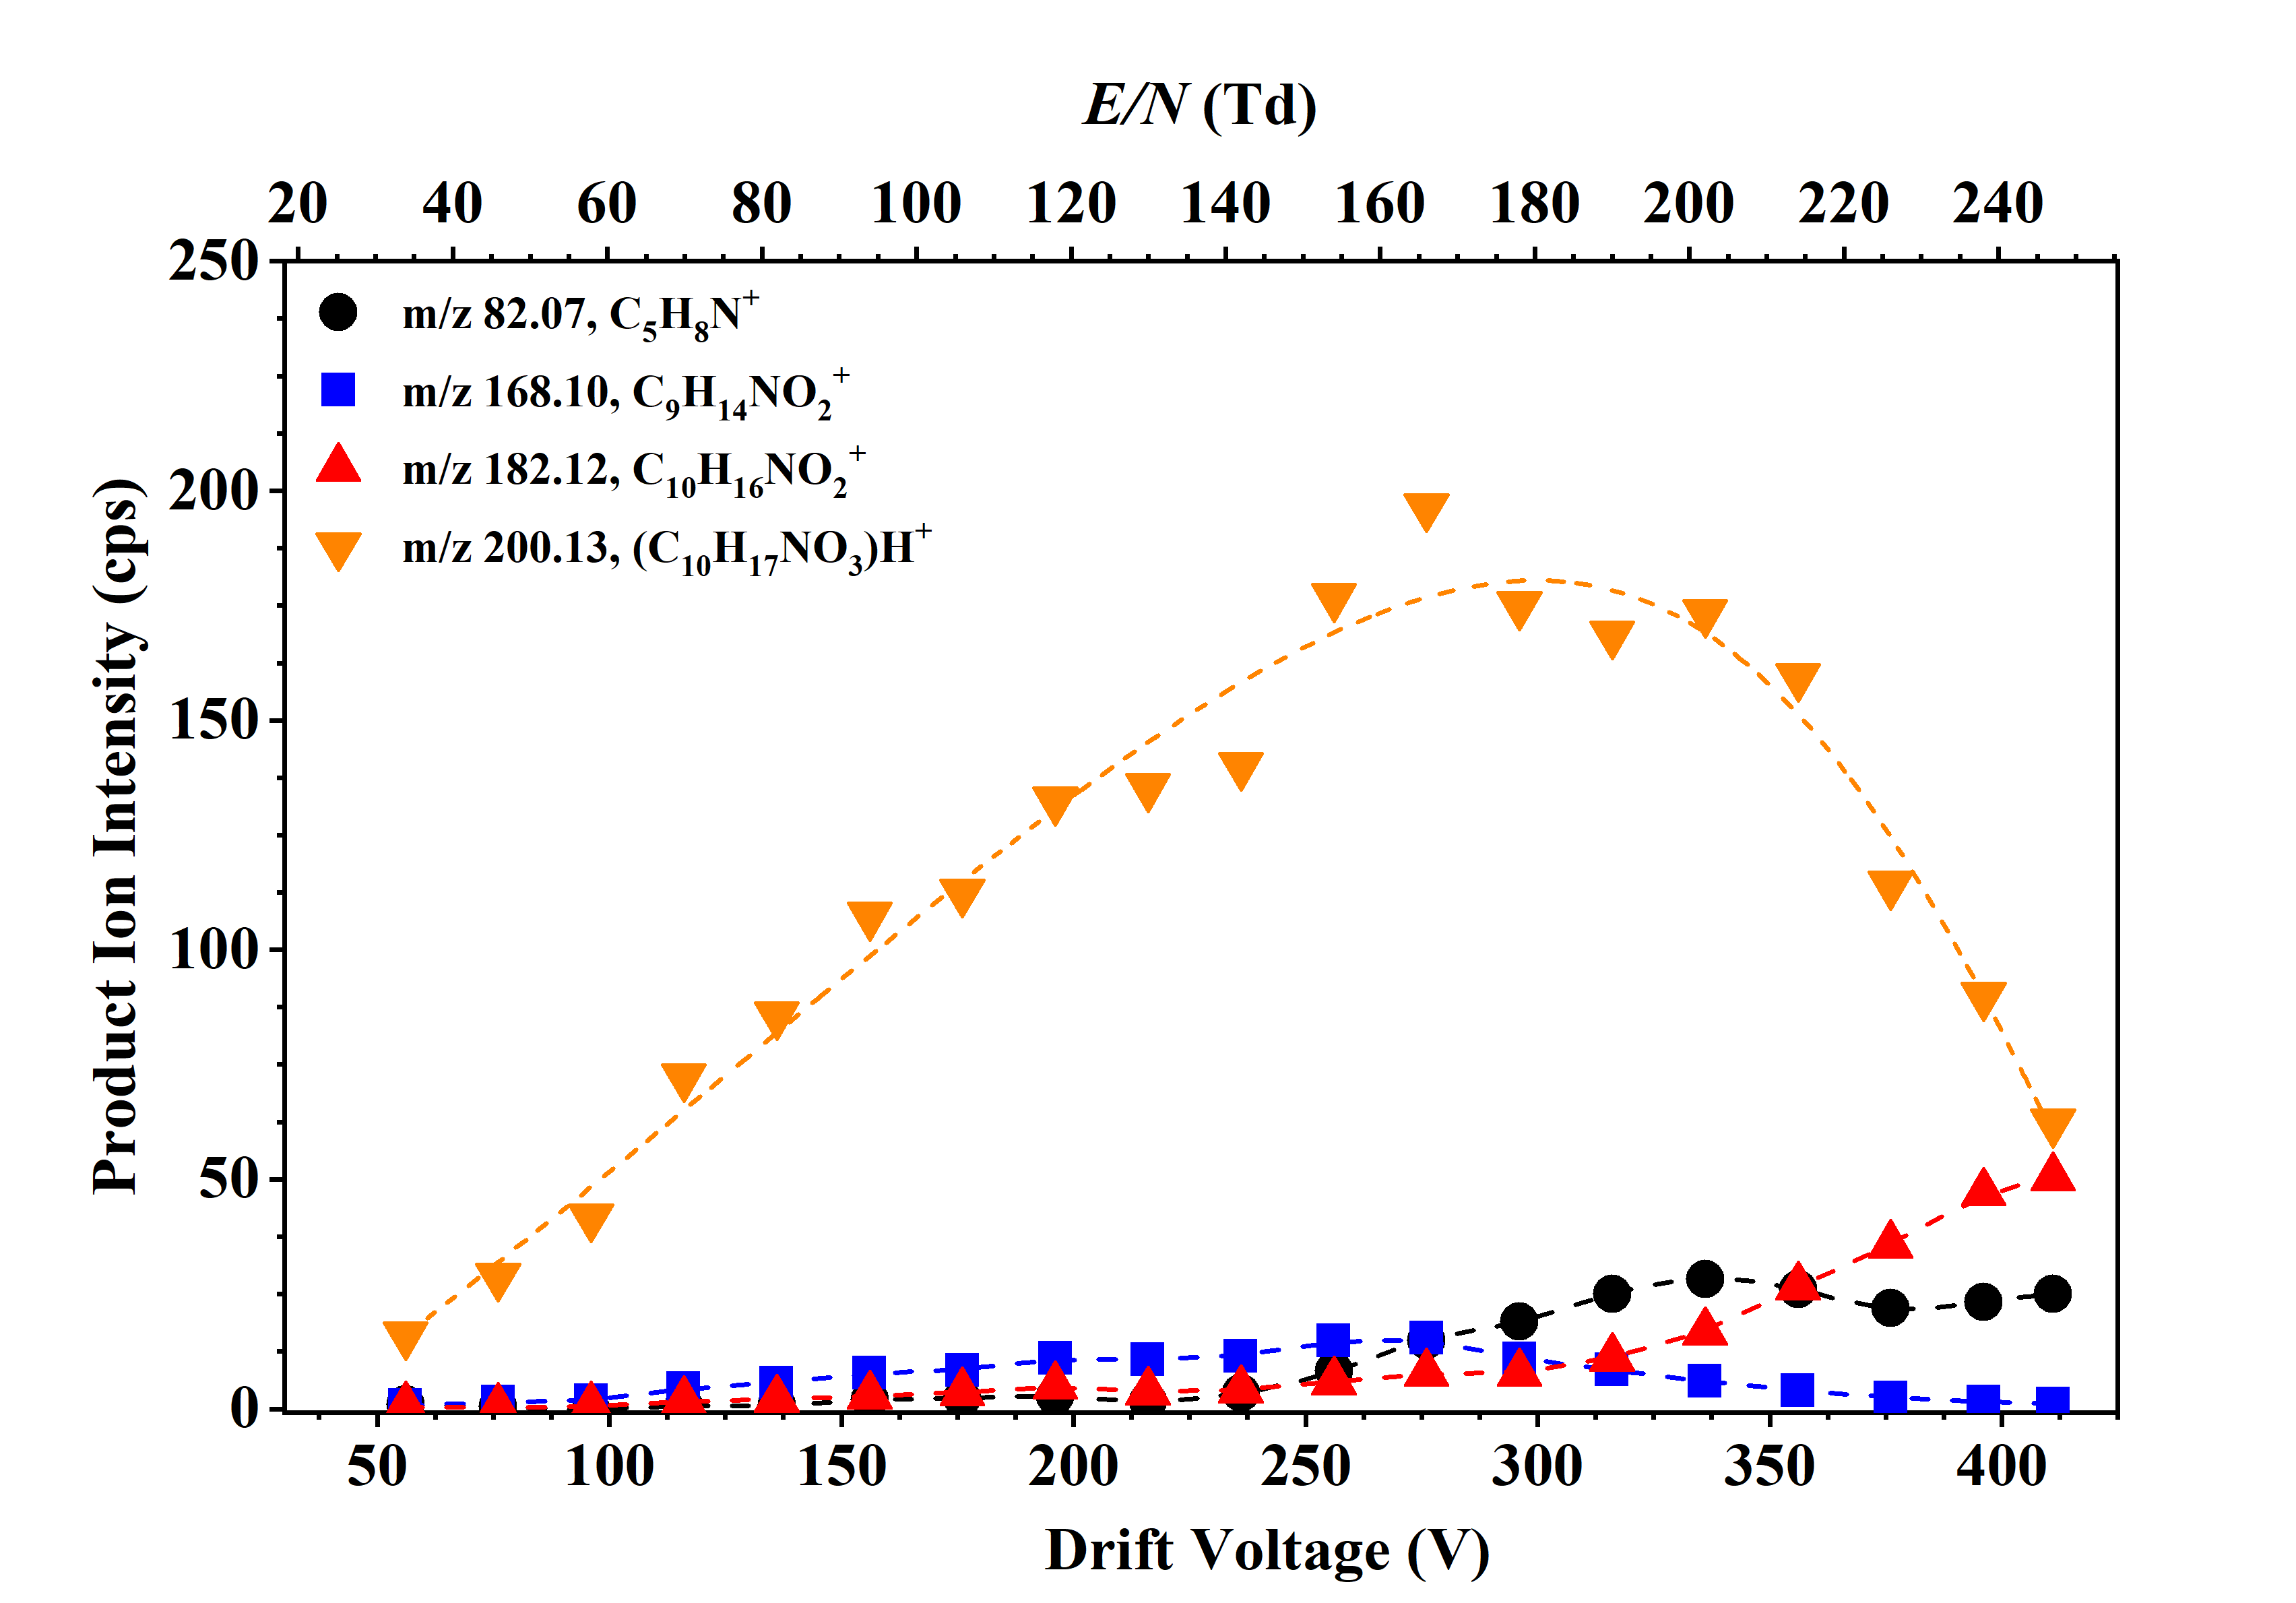
\includegraphics[width=0.8\linewidth]{pics/cocaine-chapter/MeEcg-cps.png}}\\
\sidesubfloat[]{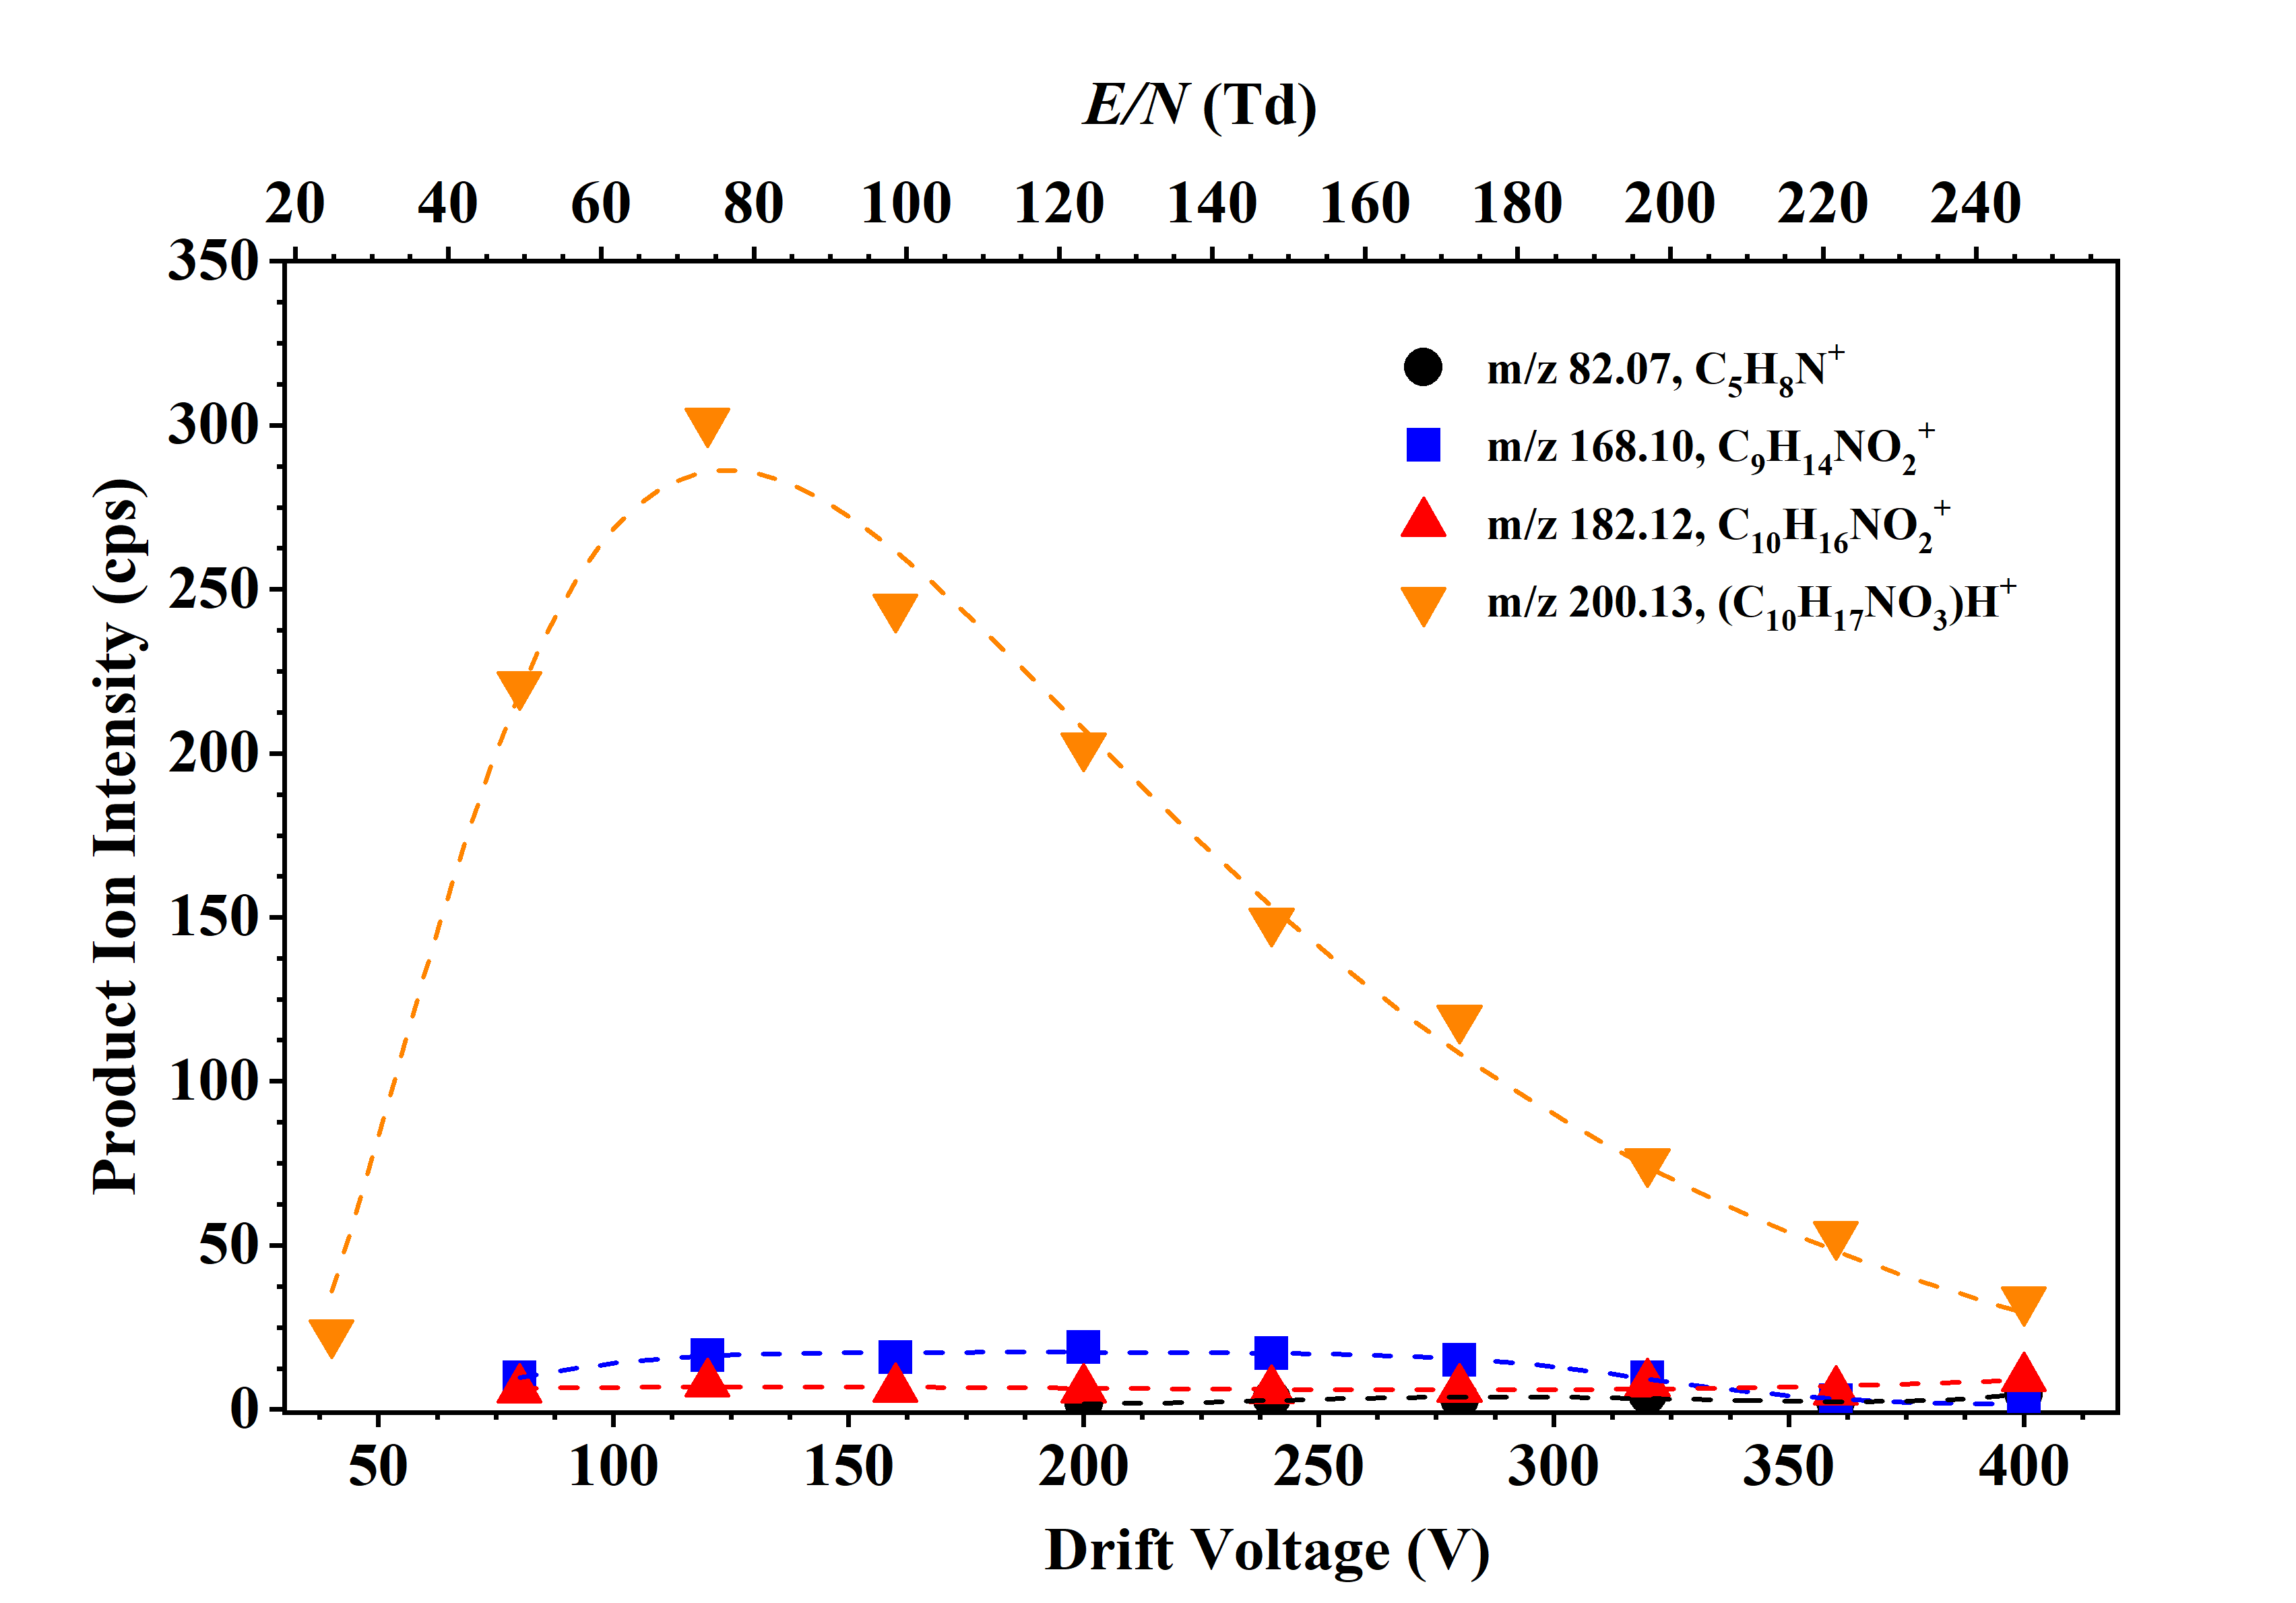
\includegraphics[width=0.8\linewidth]{pics/cocaine-chapter/humid/MeEcg-cps.png}}
\caption{Product ion signal intensities in counts per second of the product ions resulting from reactions of the H$_3$O$^+$.(H$_2$O)$_n$ (n = 0, 1, 2) with methyl ecgonine as a function of the drift voltage and the reduced electric field in (a) normal and (b) humid conditions.}
\label{fig:MeEcgEN}
\end{figure}



\autoref{tb:me2} gives the energetics of the main structures and transition states compared to those of MeEcg and H$_3$O$^+$ or (H$_2$O)H$_3$O$^+$.
%
All the structures are exergonic with H$_3$O$^+$, with the energetics for the transition state for the loss of MeOH, TS, being  similar to the transition state TS2 for cocaine.
%
This transition state consists on the barrierless dissociation of MeOH after the proton has migrated from from O3 to O5 to yield C$_9$H$_{14}$NO$_2^+$ at \textit{m/z} 168. However, direct protonation of O5 can also take place. 
%
The formation of C$_{10}$H$_{16}$NO$_2^+$ at \textit{m/z} 182  needs the proton to be on O4.
%
Then the barrierless loss of H$_2$O takes place, with further rearrangements and bond breaking to yield the structure in \autoref{fig:MeEcg_fragment}.

\begin{table}[htbp]
\centering
\caption{Energetics relative to methyl ecgonine and H$_3$O$^+$ and, in brackets, to methyl ecgonine and (H$_2$O)H$_3$O$^+$. }
\label{tb:me2}
\begin{tabular}{lccc}
\toprule
\textbf{Reaction or transition state}	&\textbf{\textit{m/z} } &\textbf{$\Delta$H$_{298}$} &\textbf{$\Delta$G$_{298}$}\\
& &	\textbf{(kJ/mol)} &\textbf{(kJ/mol)} \\  \toprule
MeEcg1H$^+$   				&	200	& -312 (-154)  & -312 (-188) \\ \midrule
(MeEcgH - MeOH)$^+$ + MeOH	&	168	& -118 (+40)  & -171 (-47)   \\ \midrule
TS for loss of MeOH			&		& +4 (+162)  	& 0 (+124)   		\\ \midrule
(MeEcgH - H$_2$O)$^+$ + H$_2$O	&	182	& -62 (+96)  & -120 (+4)   \\ 
\bottomrule
\end{tabular}
\end{table}


\begin{figure}[htbp]
\centering
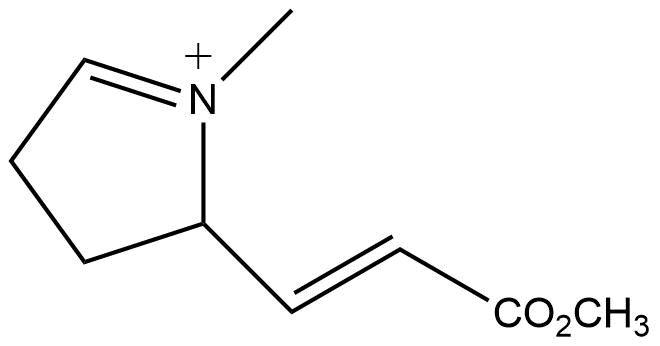
\includegraphics[width=0.3\linewidth]{pics/cocaine-chapter/meecg_frag.png}
\caption{Rearrangement of the product ion at \textit{m/z} 182 from protonated methyl ecgonine.}
\label{fig:MeEcg_fragment}
\end{figure}










%\begin{figure}[htbp]
%\centering
%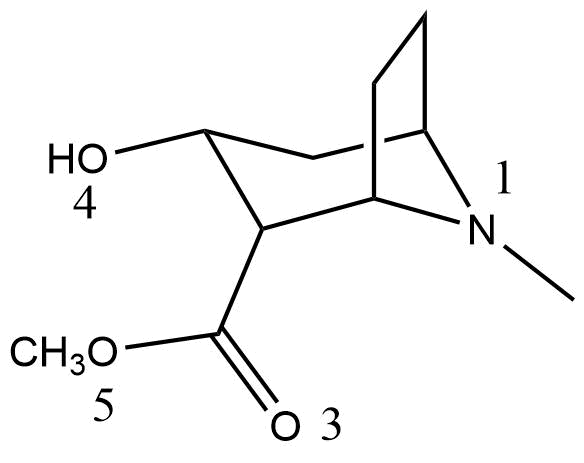
\includegraphics[width=0.3\linewidth]{pics/cocaine-chapter/MeEcg_struct.png}
%\caption{Structure  of methyl ecgonine, including the numbering of the main protonation sites.}
%\label{fig:MeEcg_struct}
%\end{figure}





%\begin{figure}[htbp]
%\centering
%\scalebox{0.5}{
%\begin{tikzpicture}
%\chemfig{[:-30]O^4(-[::180]H)>[::60](?[a])-[::45]-[::-60,1.4](<:[::60]H)(-[::-60]N^1?[b,{-}]-[::15])-[::90,1.1]-[::135,0.8]-[::45,1.1](?[b])(<[::0]H)-[::-60]?[a](<[::45](=[::60]O^3)-[::-60]O^5-[::60])}
%\end{tikzpicture}}
%\caption{Methyl ecgonine}\label{fig:me}
%end{figure}






\subsection{Benzoate esters and benzoic acid}
Benzoate esters are chemical substances with a benzene ring bonded to the carbon atom of a carboxylate ester. 
%
The benzoate moiety in cocaine has the structure of isopropyl benzoate.
%


Protonated methyl ecgonidine at \textit{m/z} 182 is a carbocation resulting from the loss of benzoic acid from the protonated cocaine molecule.
%
The proton needs to be on O2 or O4 for this fragmentation pathway to take place but a transition state yielding such configuration was not found as the proton went to O3 instead. %
For this reason benzoic acid (BzAcid) and some benzoate esters, namely ethyl benzoate (EtBz), methyl benzoate (MeBz) and isopropyl benzoate (iPrBz)  were included in the study.
%
Benzoic anhydride was also tested but with benzoic acid being a decomposition product of benzoic anhydride with lower vapour pressure, the results could be misleading and hence this compound was finally discarded.

%(A brief investigation of benzoic anhydride was attempted but the relative vapour pressures of benzoic acid and benzoic acid are such that the former dominated the spectrum and the attempt was discontinued.) 


%But we haven’t found it yet!!!!!!!!!!!!!!!

 
 \autoref{tb:bz1} shows the proton affinity and Gibbs free energy of the protonation sites that yield the two most stable structures of protonated benzoic acid and methyl, ethyl and isopropyl benzoate.
 %
 The suffix 1H$^+$ is used here to name protonated molecules with the proton on O1 (i.e. the carbonyl oxygen) while  2H$^+$ refers to the proton is in O2 (i.e. the alkoxy oxygen).
 %
 These protonation sites are indicated in \autoref{tab:structs2}. 
%

 
 
 
%\begin{figure}[htbp]
%\centering
%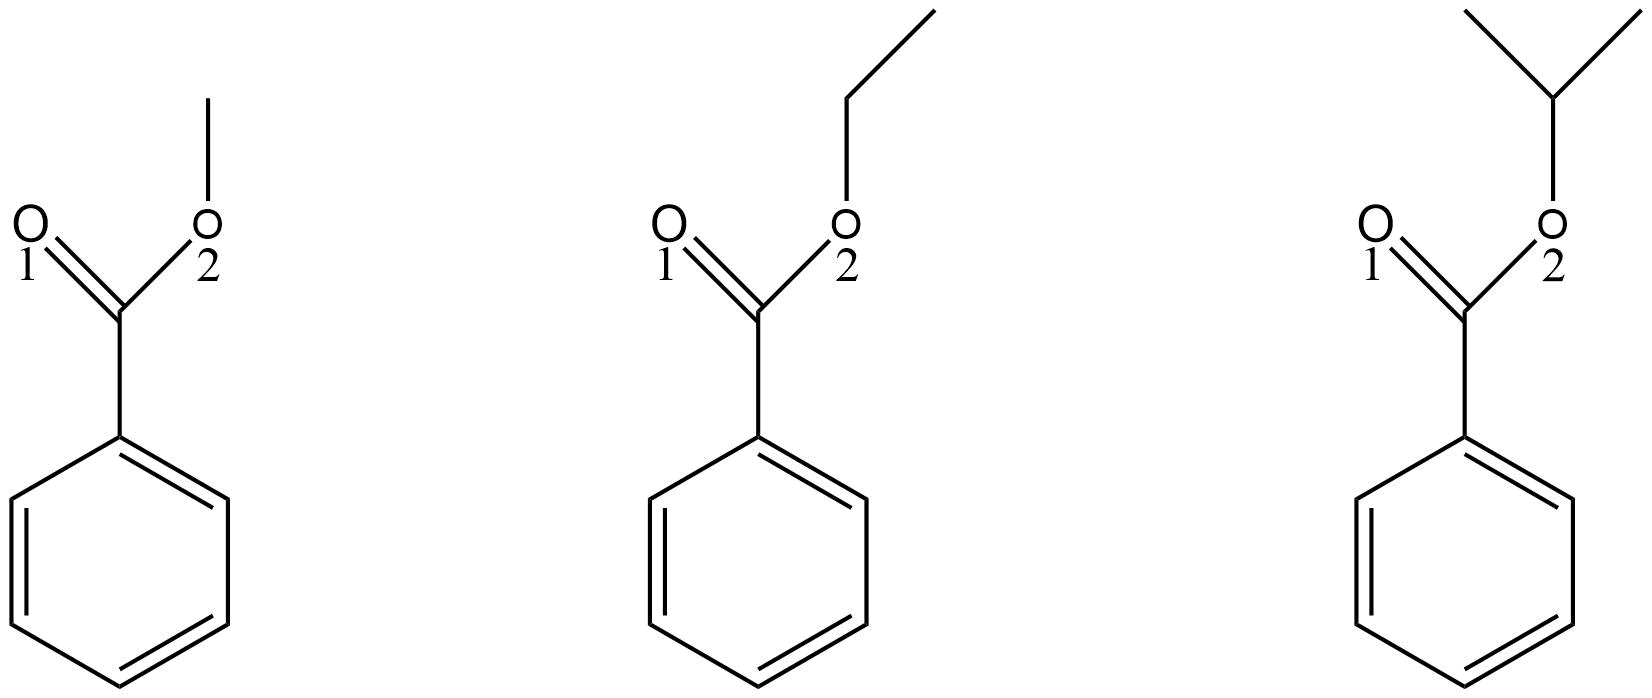
\includegraphics[width=0.6\linewidth]{pics/cocaine-chapter/benzoates_struct.png}
%\caption{Structure  of (left) methyl benzoate, (centre) ethyl benzoate and (right) isopropyl benzoate.}
%\label{fig:benzoate_struct}
%\end{figure} 


\begin{table}[htbp]
\centering
\caption{Proton affinity and Gibbs free energy of the main protonation sites of benzoic acid, methyl benzoate, ethyl benzoate and isopropyl benzoate.}
\label{tb:bz1}
\begin{tabular}{lcc}
\toprule
\textbf{Structure} &\textbf{PA (kJ/mol)} &\textbf{GB (kJ/mol)}\\ \toprule
BzAcid1H$^+$   &812 &783 \\
BzAcid2H$^+$   &724 &741 \\\midrule
MeBz1H$^+$ &	839	&808\\
MeBz2H$^+$ &	764	&741\\\midrule
EtBz1H$^+$ &	859	& 831\\
EtBz2H$^+$ &	779	& 750\\\midrule
iPrBz1H$^+$	&861	&831\\
iPrBz2H$^+$	&786	&760\\
\bottomrule
\end{tabular}
\end{table}
	
	

 
\subsubsection{Methyl benzoate}
The most stable structure of protonated MeBz  is that with the proton on the carbonyl oxygen O1 (i.e. MeBz1H$^+$), whose proton affinity and Gibbs free energy are  839 and 808 kJ mol$^{-1}$. Thus MeBz can undergo proton transfer from H$_3$O$^+$ and (H$_2$O)H$_3$O$^+$ only and not from higher order water cluster ions.
%
Proton transfer from (H$_2$O)H$_3$O$^+$ to MeBz yields MeBz1H$^+$, while proton transfer from H$_3$O$^+$ can result in either MeBz1H$^+$ or MeBz2H$^+$.

The product ion intensities as a function of the drift voltage and the reduced electric field for the reaction of MeBz with (H$_2$O)$_n$H$_3$O$^+$ (n = 0, 1) are given in \autoref{fig:MeBzEN} and the energetics for the formation of the main product ions resulting from this reaction are provided in \autoref{tb:mb2}. 
%
The most abundant for most of the studied \textit{E/N} range is the protonated parent molecule.
%
Only at more 230 Td in the normal conditions measurement other product ions are significantly more intense: \textit{m/z} 77 and \textit{m/z} 91. 
%
Also, clustering of MH$^+$ with H$_2$O at \textit{m/z} 155 is observed at low \textit{E/N} in the humid case.

\begin{figure}[htbp]
\centering
\sidesubfloat[]{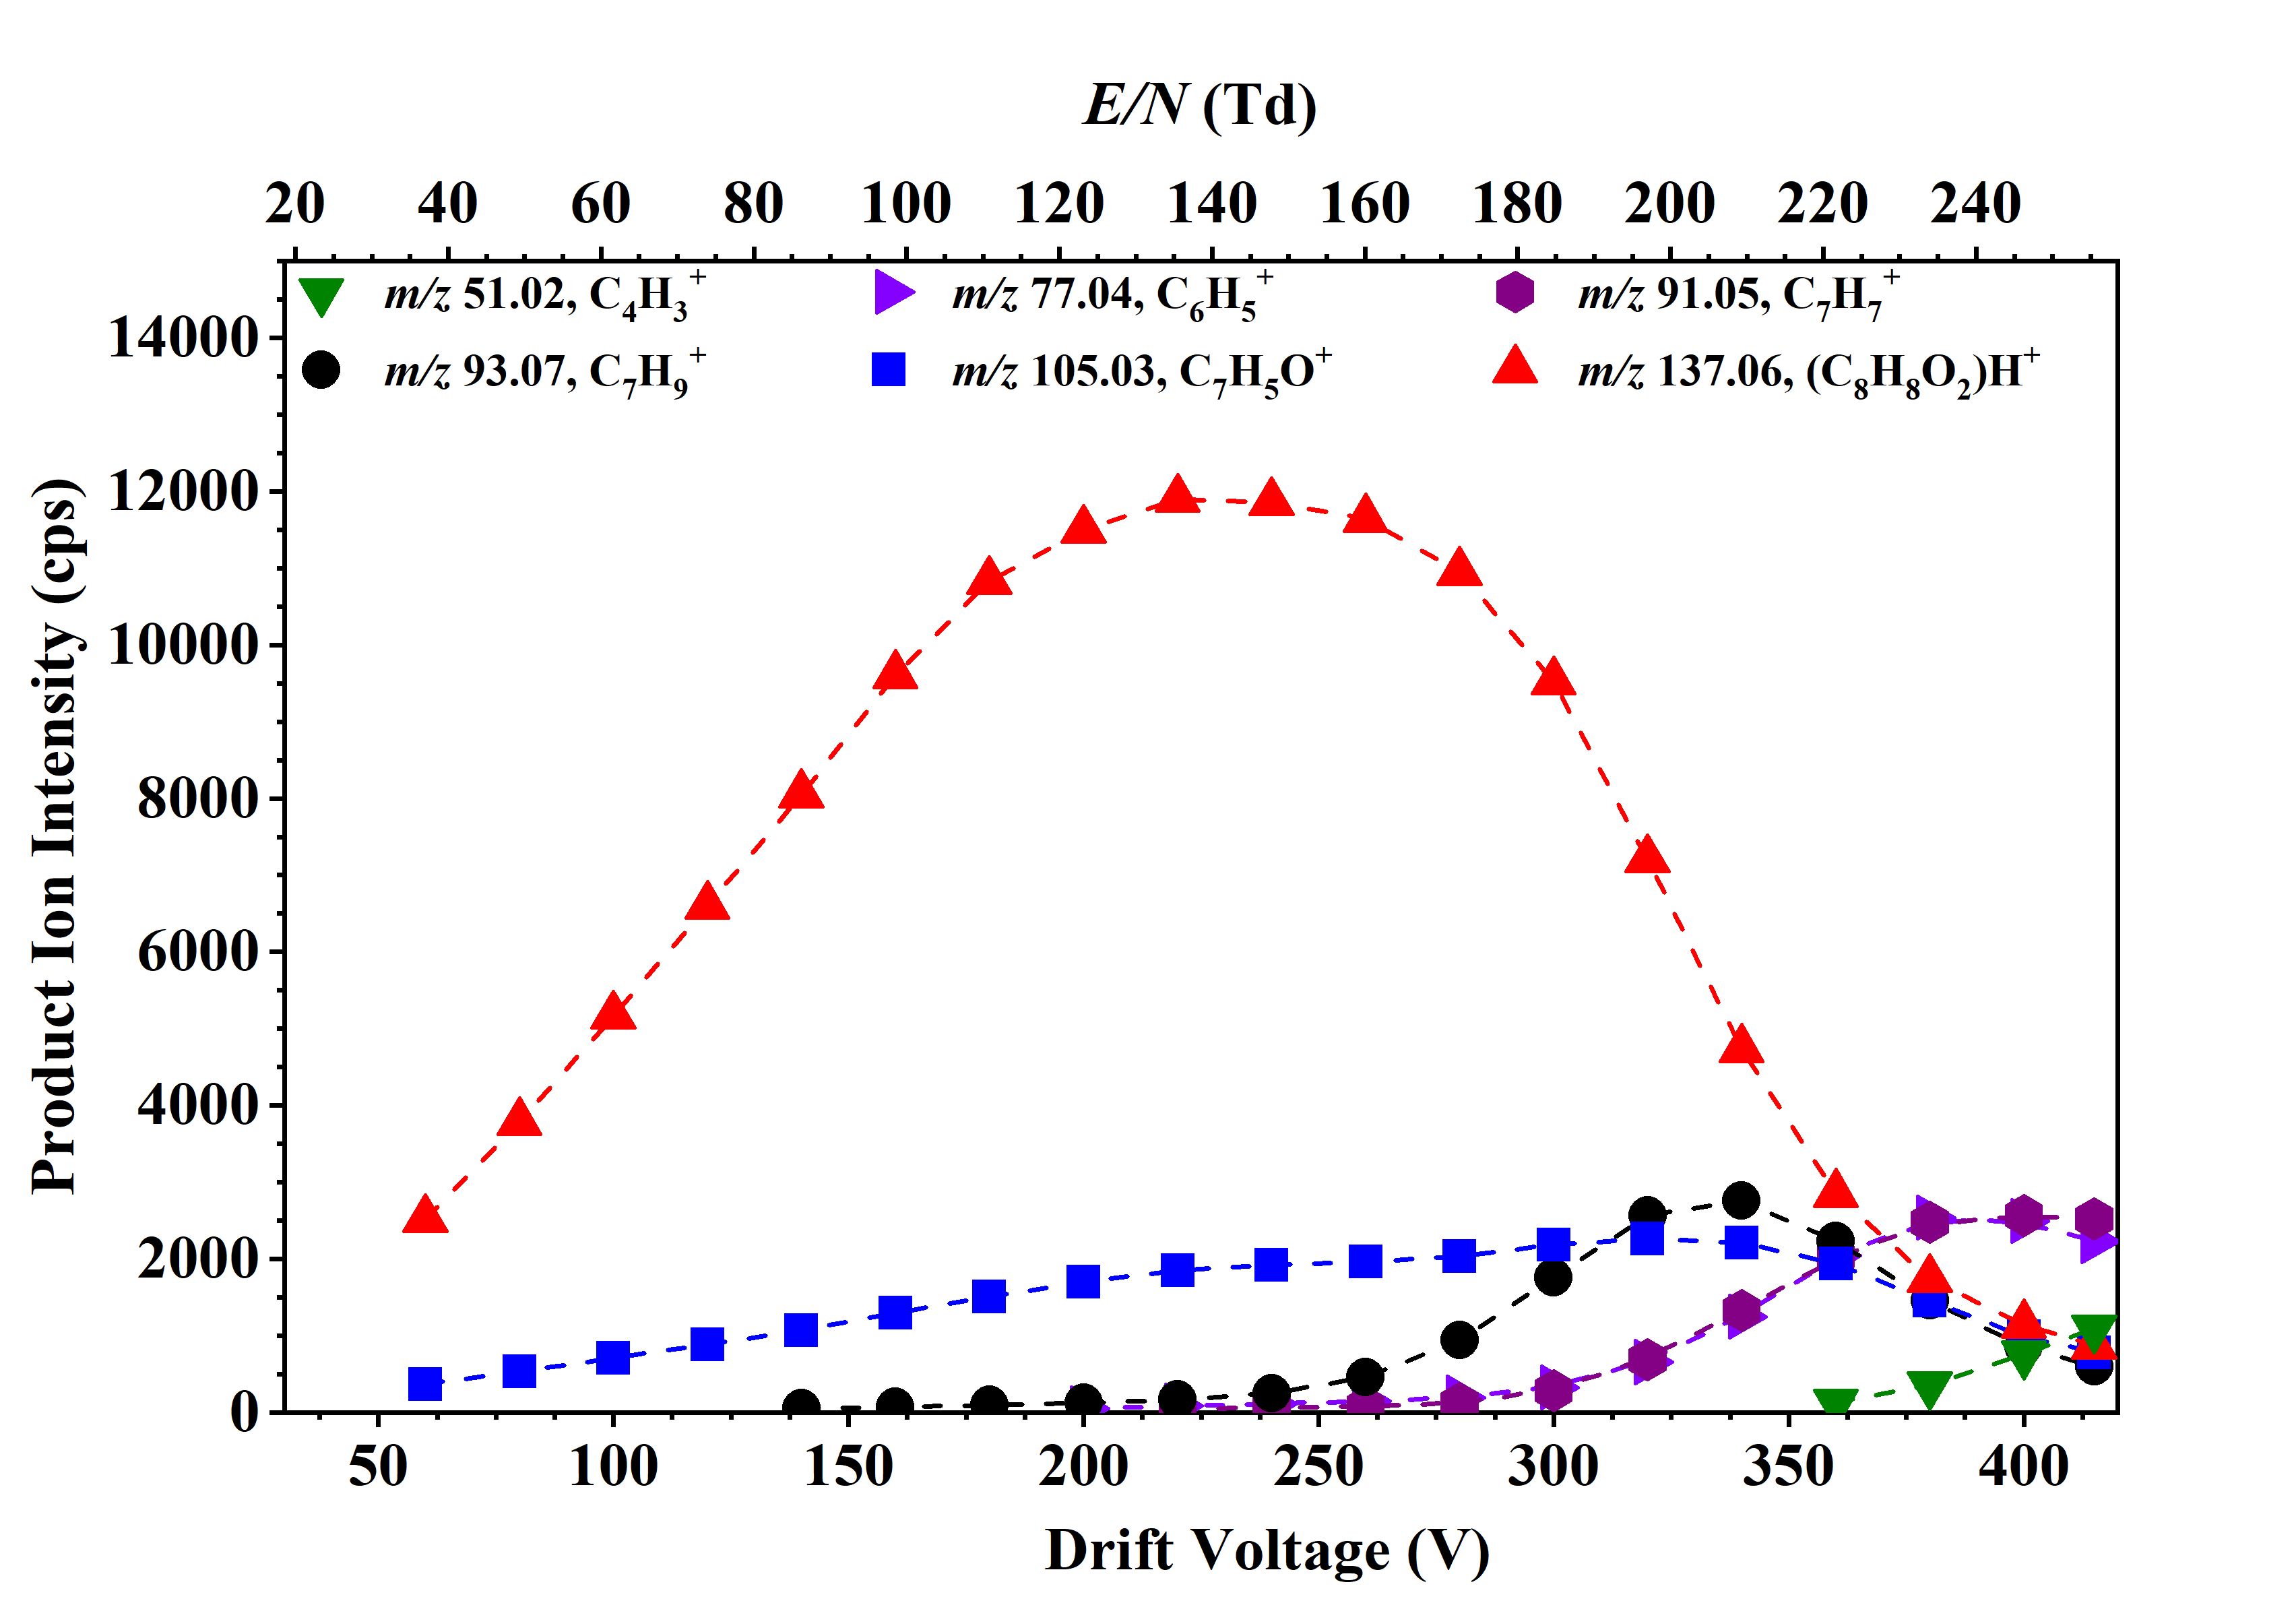
\includegraphics[width=0.8\linewidth]{pics/cocaine-chapter/MeBz-cps2.png}}\\
\sidesubfloat[]{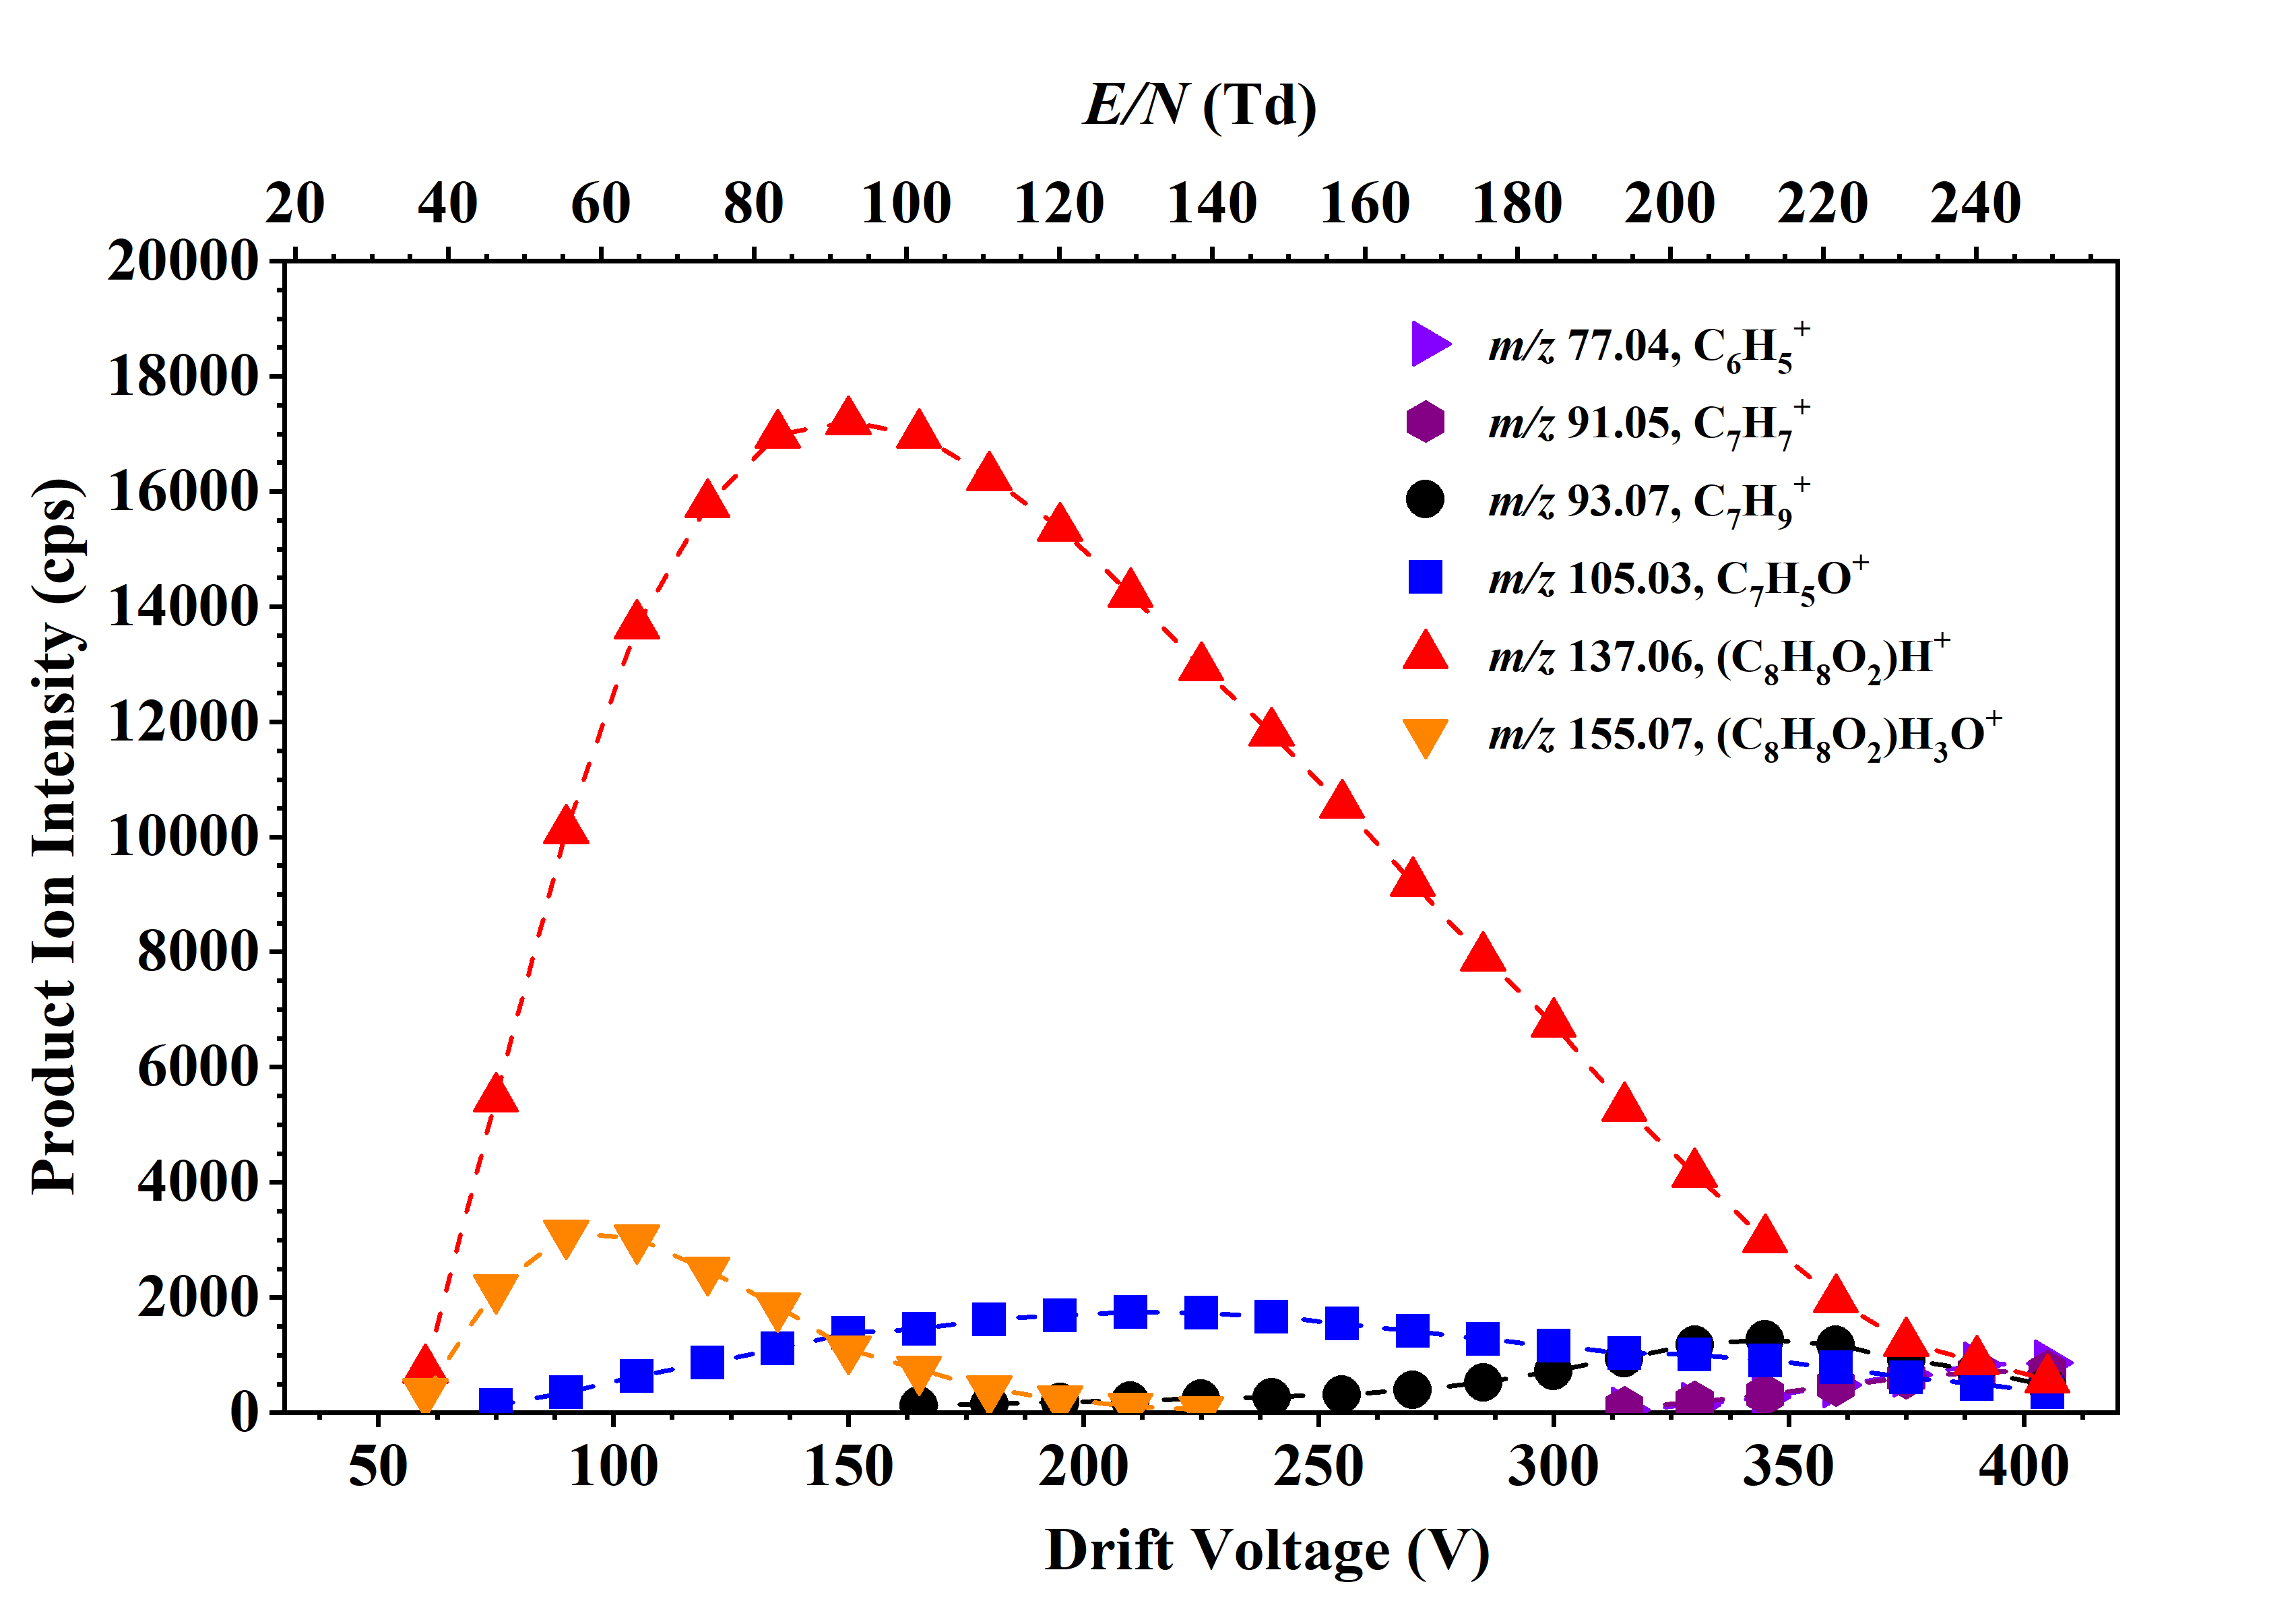
\includegraphics[width=0.8\linewidth]{pics/cocaine-chapter/humid/MeBz-cps.png}}
\caption{Product ion signal intensities in counts per second of the product ions resulting from reactions of the H$_3$O$^+$.(H$_2$O)$_n$ (n = 0, 1) with methyl benzoate as a function of the drift voltage and the reduced electric field in (a) normal and (b) humid conditions..}
\label{fig:MeBzEN}
\end{figure}

\begin{table}[htbp]
\centering
\caption{Energetics relative to methyl benzoate and H$_3$O$^+$ and, in brackets, to methyl benzoate and (H$_2$O)H$_3$O$^+$. }
\label{tb:mb2}
\begin{tabular}{lccc}
\toprule
\textbf{Reaction or transition state}	&\textbf{\textit{m/z} } &\textbf{$\Delta$H$_{298}$} &\textbf{$\Delta$G$_{298}$}\\
& &	\textbf{(kJ/mol)} &\textbf{(kJ/mol)} \\  \toprule
MeBz1H$^+$   					&	137	& -155 (+3)  & -155 (-31)   \\ \midrule
MeBz2H$^+$ 						&	137	& -80 (+78)  & -88 (+36)    \\ \midrule
Benzoyl$^+$ + MeOH				&	105	& -29 (+134)  & -82 (+42)   \\ \midrule
TS 1H$^+$ to 2H$^+$                     &		& +15 (+173)  	& +14 (+138)\\ \midrule
C$_7$H$_9^+$ + CO$_2$           &   93  &   -188 (-20) & -228 (-104) \\
\bottomrule
\end{tabular}
\end{table}


% loss of MeOH
Benzoyl$^+$ (C$_7$H$_5$O$^+$) at \textit{m/z} 105 comes from the barrierless loss of MeOH from MeBz2H$^+$. 
%
This needs the proton on O2, which can occur following two different pathways: (i) direct protonation of O2 from H$_3$O$^+$ resulting in MeBz2H$^+$, or (ii) migration of the proton from O1 to O2.
%
When the proton is on O2 (i.e. MeBz2H$^+$) loss of MeOH occurs through the barrierless breaking of the C--O bond. 
%
The difference between the two pathways lies in the energetics. 
%
Direct protonation of O2 is exergonic, while for the migration of the proton following protonation of O1 an endergonic transition state was found and hence the loss of MeOH following this pathway will only occur at collisional energies that are high enough to overcome said transition state.
%
It is not possible to directly distinguish which of the pathways (if not both) is operating but it was found that direct protonation of O2 in EtBz occurs, which suggests that the same happens with MeBz (see subsection \ref{section:etbz}). 


The other observed product ions are fragments generated through field-activated collision-induced dissociation. 
%
These are found at \textit{m/z} 93, \textit{m/z} 91, \textit{m/z} 77 and \textit{m/z} 51.
%
Protonated toluene (C$_7$H$_9^+$) is found at \textit{m/z} 93 resulting from the loss of CO$_2$ from MeBz1H$^+$.
%
Although the formation of this ion is exergonic (see \autoref{tb:mb2}), it is only observed at high reduced electric fields, which indicates that there must be a transition state with high  requirements in terms of energy. 
%
This ion will not be further considered, neither will those resulting from its fragmentation at higher \textit{E/N}:
C$_7$H$_7^+$ at \textit{m/z} 91 (loss of H$_2$ from \textit{m/z} 93),
C$_6$H$_5^+$ at \textit{m/z} 77 (loss of CH$_4$ from \textit{m/z} 93), 
and
C$_4$H$_3^+$ at \textit{m/z} 51 (loss of CH$_2$ from \textit{m/z} 77), which is only observed in the normal conditions experiment at very high \textit{E/N} (>220 Td).














\subsubsection{Ethyl benzoate}\label{section:etbz}

Similarly to MeBz, EtBz can undergo proton transfer from (H$_2$O)$_n$H$_3$O$^+$ for n = 0 and 1.
%, with EtBz1H$^+$ being the result of the reaction with either (H$_2$O)H$_3$O$^+$ or H$_3$O$^+$, but only the reaction with H$_3$O$^+$ can result in EtBz2H$^+$.
%
The product ion intensities as a function of the drift voltage and the reduced electric field for the reaction of EtBz with (H$_2$O)$_n$H$_3$O$^+$ (n = 0, 1) are given in \autoref{fig:EtBzEN} and the energetics for the formation of the main product ions resulting from this reaction are provided in \autoref{tb:eb2}. 

\begin{figure}[htbp]
\centering
\sidesubfloat[]{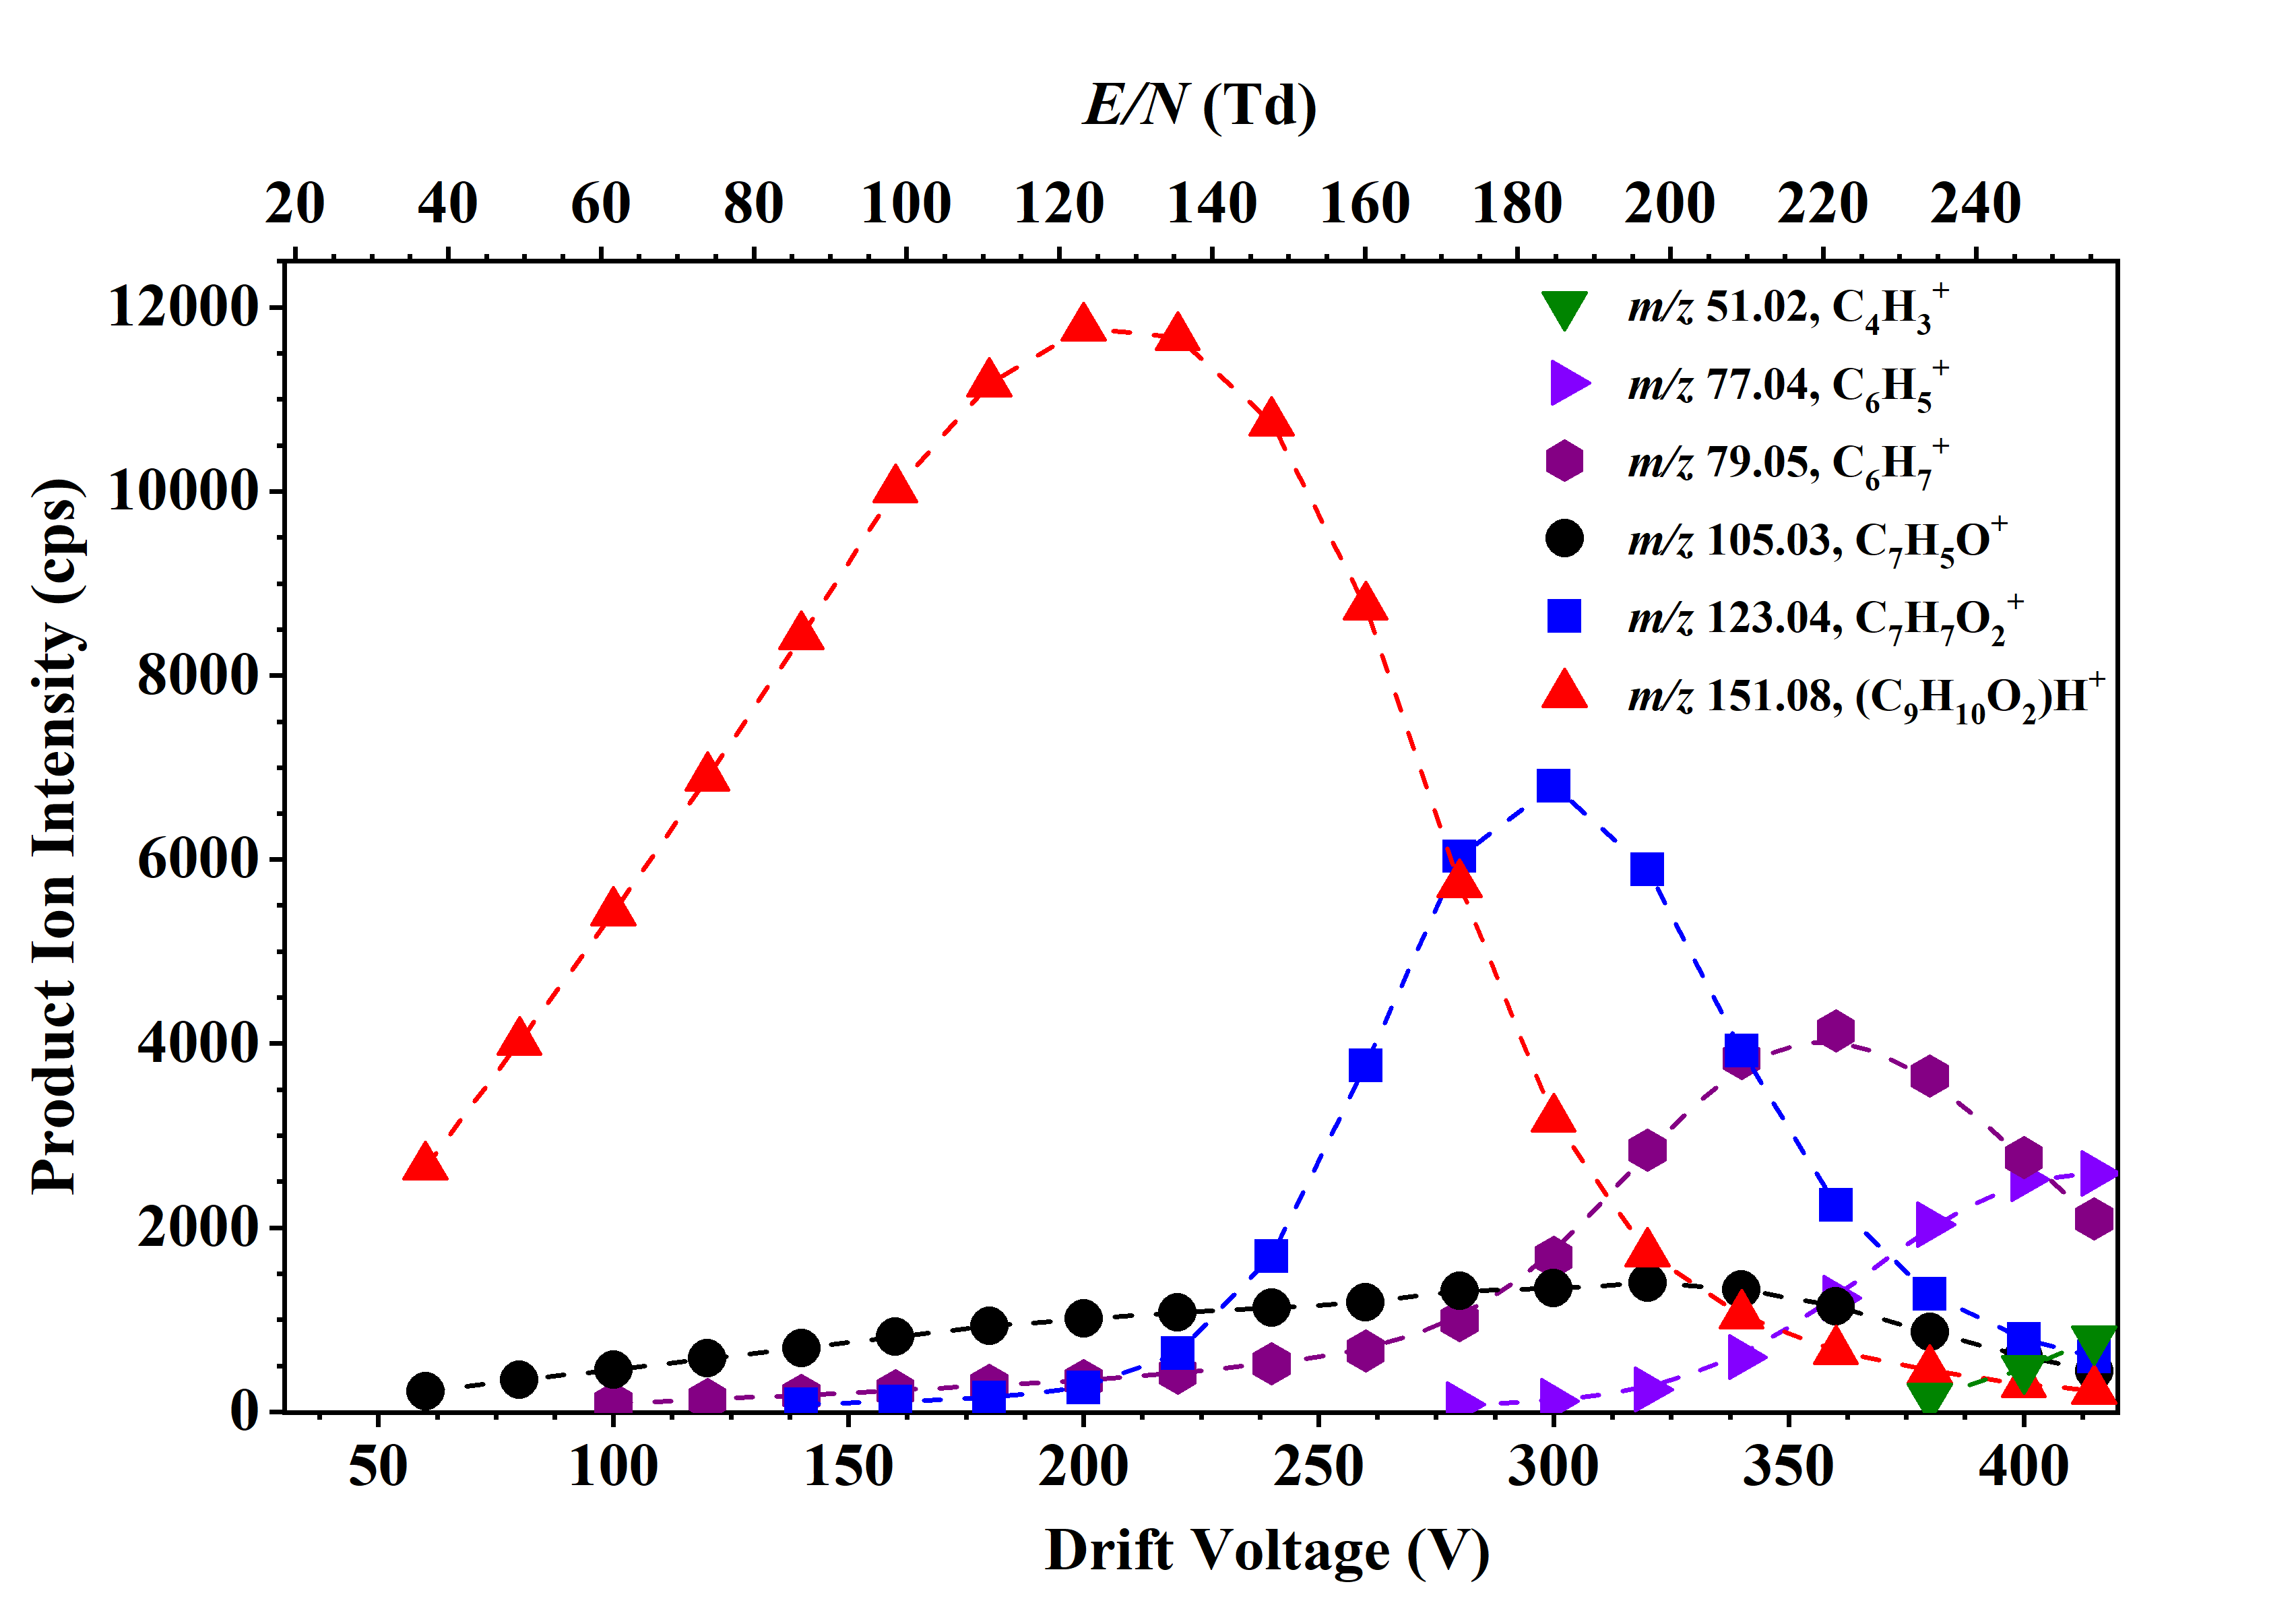
\includegraphics[width=0.8\linewidth]{pics/cocaine-chapter/EtBz-cps.png}}\\
\sidesubfloat[]{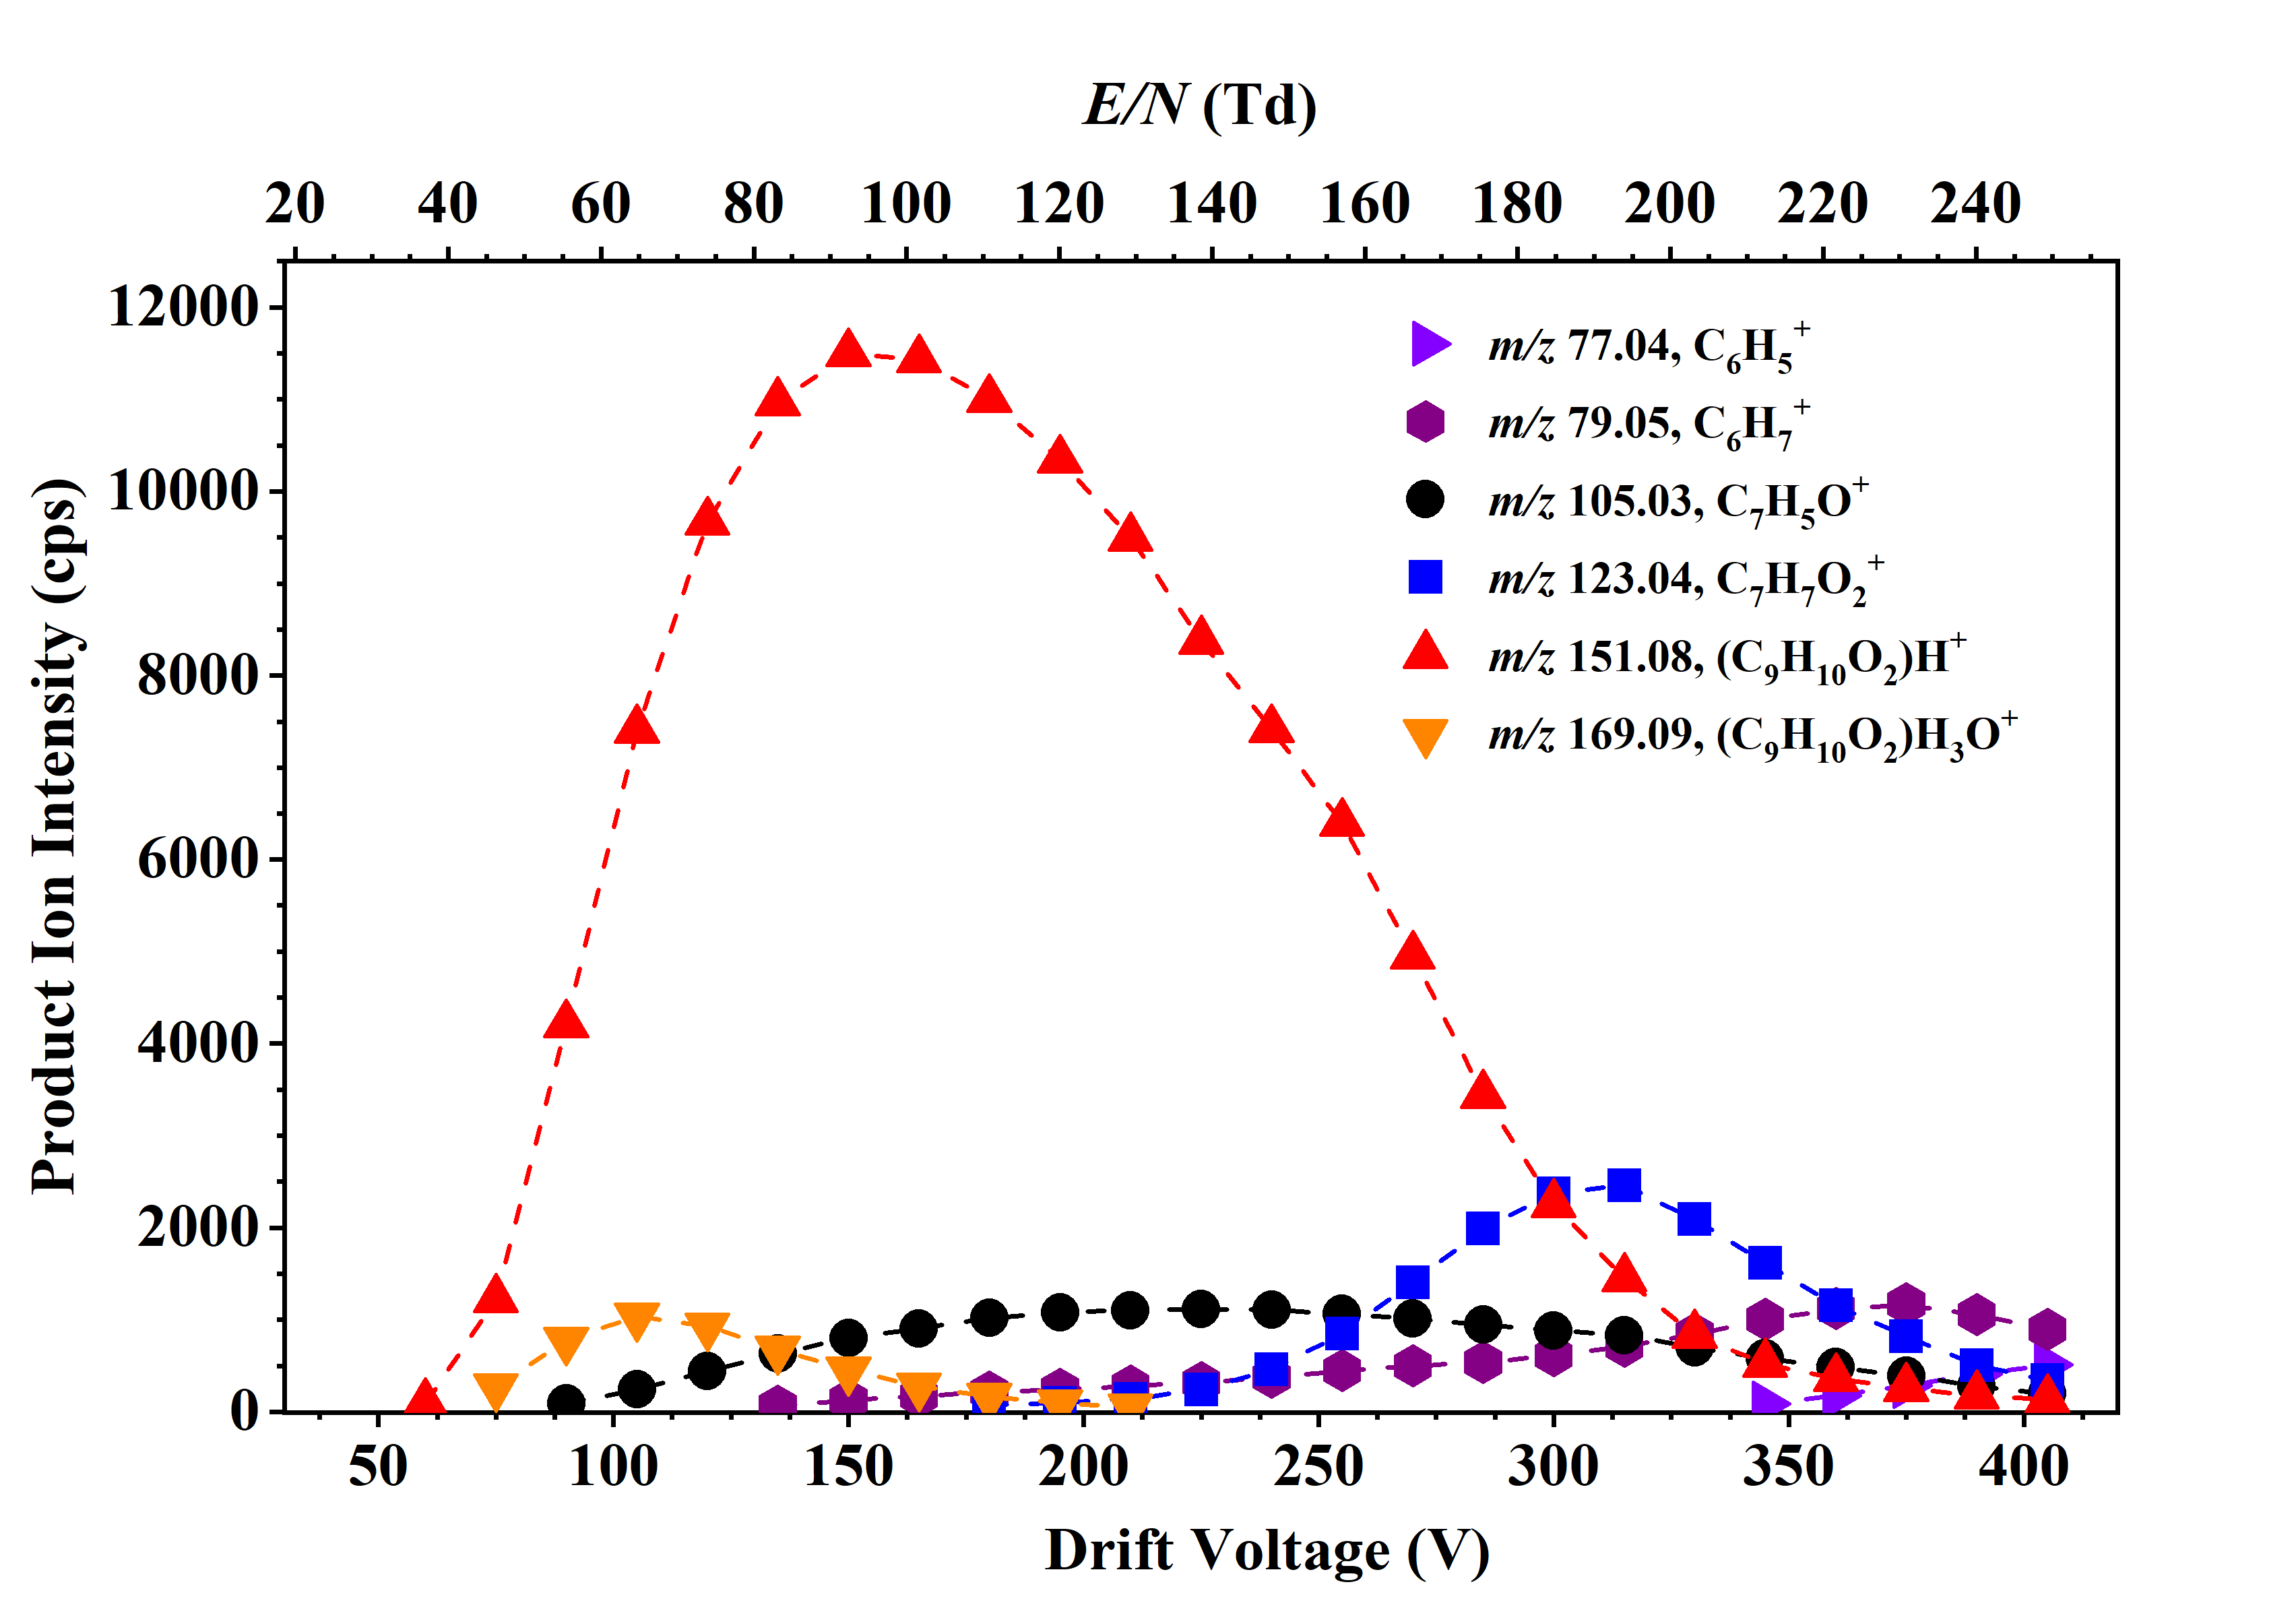
\includegraphics[width=0.8\linewidth]{pics/cocaine-chapter/humid/EtBz-cps.png}}
\caption{Product ion signal intensities in counts per second of the product ions resulting from reactions of the H$_3$O$^+$.(H$_2$O)$_n$ (n = 0, 1) with ethyl benzoate as a function of the drift voltage and the reduced electric field in (a) normal and (b) humid conditions.}
\label{fig:EtBzEN}
\end{figure}


\begin{table}[htbp]
\centering
\caption{Energetics relative to ethyl benzoate and H$_3$O$^+$ and, in brackets, to ethyl benzoate and (H$_2$O)H$_3$O$^+$. }
\label{tb:eb2}
\begin{tabular}{lccc}
\toprule
\textbf{Reaction or transition state}	&\textbf{\textit{m/z} } &\textbf{$\Delta$H$_{298}$} &\textbf{$\Delta$G$_{298}$}\\
& &	\textbf{(kJ/mol)} &\textbf{(kJ/mol)} \\  \toprule
EtBz1H$^+$   					&	151	& -180 (-22)  & -178 (-54)   \\ \midrule
EtBz2H$^+$   					&	151	& -95 (+63)  & -97 (+27)   \\ \midrule
Benzoyl$^+$  + EtOH				&	105	& -36 (+122)  & -83 (+41)   \\ \midrule
TS 1H$^+$ to 2H$^+$		&		& -3 (+155)  & +2 (+126)   \\ \midrule
BzAcidH$^+$ + C$_2$H$_4$	&	123	& -74 (+84)  & -120 (+4)   \\ \midrule
TS1 for loss of ethene from 1H$^+$	&		& -36 (+122)  & -41 (+83)   \\ \midrule
TS2 for loss of ethene from 2H$^+$	&		& -15 (+143)  & -14 (+110)   \\ \midrule
Benzoyl$^+$  + C$_2$H$_4$ + H$_2$O	&	105	& +15 (+173)  & -77 (+47)  \\ \midrule
TS3 for loss of H$_2$O from BzAcidH$^+$&	& +98 (+256)  & +52 (+176)   \\ \midrule
%\multicolumn{2}{l}{TS3 to above(loss of H$_2$O from BzAcidH$^+$)}		& +98  & +52   \\ \midrule
%TS3 to above, i.e.	&		&   &    \\ 
%loss of H$_2$O from BzAcidH$^+$	&		& +98  & +52   \\ \midrule
BenzeneH$^+$ + C$_2$H$_4$ + CO$_2$	 &	79	& +34 (+192)  & -132 (-8)  \\ 
\bottomrule
\end{tabular}
\end{table}


The dominant ion at low \textit{E/N} (i.e. up to ca. 170 Td in normal conditions and ca. 180 Td in humid conditions) is the protonated parent EtBzH$^+$.
%
%The differences between the abundance of EtBzH$^+$ and BzAcidH$^+$ at \textit{m/z} 123 (i.e. loss of ethene, C$_2$H$_4$) in normal and humid conditions can be explained in terms of the reagent ions abundance, as proton transfer from (H$_2$O)H$_3$O$^+$ yields EtBzH$^+$ (with the structure EtBz1H$^+$), while proton transfer from H$_3$O$^+$ can also yield fragmentation, besides EtBzH$^+$, result in 
%
%
As the first experiment that was done was that in humid conditions, it was initially thought that the large amounts of EtBzH$^+$ (presumably with the structure EtBz1H$^+$) that were observed  were the result of proton transfer from (H$_2$O)H$_3$O$^+$ and that proton transfer from H$_3$O$^+$ would always result in loss of ethene  (C$_2$H$_4$), yielding BzAcidH$^+$ at \textit{m/z} 123. The energetics in \autoref{tb:eb2} support this argument because the two transition states for the loss of ethene from EtBz1H$^+$ and EtBz2H$^+$(i.e. TS1 and TS2) are exergonic upon proton transfer from H$_3$O$^+$.
%
But the experiment in normal conditions in \autoref{fig:EtBzEN}a (with substantially less (H$_2$O)H$_3$O$^+$ reagent ions, as \autoref{fig:RI_coc}a shows) demonstrates that this argument is not correct because the \textit{m/z} 123 signal for normal and humid conditions are quite similar, with a shift of only 5 - 10 Td, and hence the loss of ethene from EtBzH$^+$ to yield BzAcidH$^+$ is the result of field-activated collision-induced dissociation.
%
In other words, loss of ethene from the protonated parent is kinetically rather than thermodynamically driven.



%Direct protonation of O2 occurs as benzoyl is observed,,,,,,,,,





%That large amounts of EtBzH$^+$ are observed at low values of \textit{E/N} demonstrates that a major reagent ion is (H$_2$O)H$_3$O$^+$ as protonation by H$_3$O$^+$ would lead to direct fragmentation to ethene and benzoic acidH$^+$. This conclusion may however be simplistic. Loss of EtOH occurs at all values of \textit{E/N}. But the expected loss of C$_2$H$_4$ only occurs as \textit{E/N} is increased. It is not possible to determine what proportion of this is due to H$_3$O$^+$ being formed at higher \textit{E/N} and what to collisional activation of EtBzH$^+$ by the field. 
%
%%An additional factor is that as \textit{E/N} increases so does the internal energy of H$_3$O$^+$.%not right

The benzoyl$^+$ cation at \textit{m/z} 105, which was observed at all \textit{E/N} values, can be formed through two different pathways:
(i) loss of ethanol from EtBzH$^+$, or
(ii) loss of ethene from BzAcidH$^+$.
%
The second fragmentation needs to overcome the endergonic transition state TS3 (+52 kJ mol$^{-1}$ relative to H$_3$O$^+$), which could be achieved through CID at high \textit{E/N}, but, since \textit{m/z} 105 is observed for the whole \textit{E/N} range, it must be formed through the loss of ethanol from protonated ethyl benzoate.
%
This requires direct protonation of O2 to give the structure EtBz2H$^+$, because the transition state TS 1H$^+$ to 2H$^+$ is slightly endergonic.


\begin{figure}[htbp]
\centering
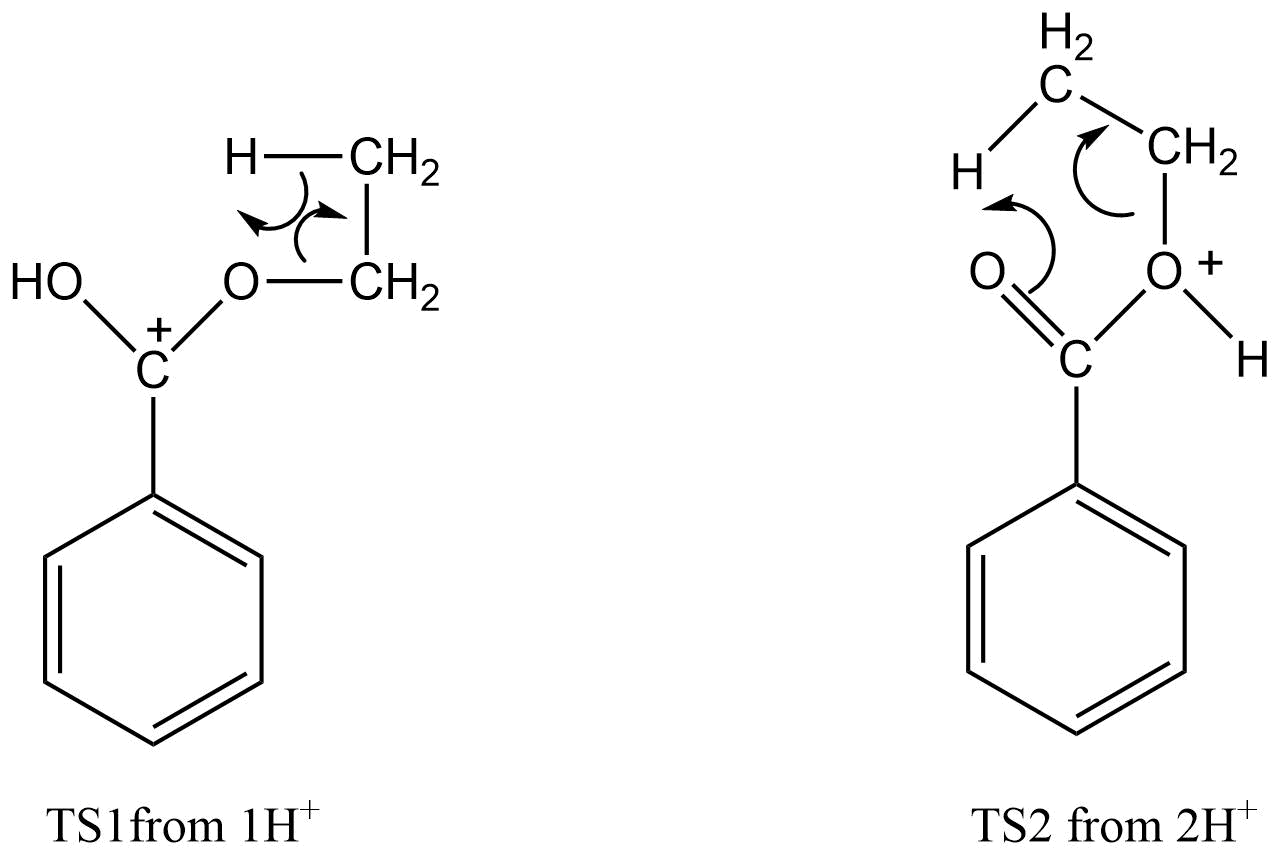
\includegraphics[width=0.5\linewidth]{pics/cocaine-chapter/etbz_ts.png}
\caption{Structure of the two transition states for the loss of ethene  from protonated ethyl benzoate.}
\label{fig:etbz_ts}
\end{figure}

The two transitions TS1 and TS2 for the loss of ethene from EtBz1H$^+$ and EtBz2H$^+$ are given in \autoref{fig:etbz_ts}.
%
Although TS2 is thermodynamically feasible, it needs direct protonation of O2 to yield EtBz2H$^+$ because the transition state EtBz1H$^+$ to EtBz2H$^+$ is endergonic.
%
EtBz2H$^+$ then fragments to benzoyl$^+$ through the barrierless dissociation of ethanol, rather than to BzAcidH$^+$ through TS2, as the former process has lower energy requirements.
%
The presence of \textit{m/z} 105 means that direct protonation of O2 to give EtBz2H$^+$ happens.
%
Likewise, the loss of ethanol to yield \textit{m/z} 105 from EtBz1H$^+$ could happen through the transition state TS EtBz1H$^+$ to EtBz2H$^+$, but the loss of ethene through TS1 is more energetically favourable.
%
The loss of ethene to BzAcidH$^+$ is thus concluded to happen through TS1.

The question that arises now is why the ion with \textit{m/z} 105 (i.e. the loss of ethanol from EtBz2H$^+$) is found at low \textit{E/N} while the ion with \textit{m/z} 123 is only found at high \textit{E/N}.
%
This can be better understood with the $\Delta$G plot as a function of the reaction coordinate in \autoref{fig:etbz_deltag}.
%
%
%
%
%Loss of ethene via TS1 is the most likely pathway. 
%Whilst TS2 is exergonic it requires EtBz2H$^+$ to be formed directly as the TS for the shift 1H$^+$ to 2H$^+$ is much higher than the elimination of ethene via TS1. 
%Moreover EtBz2H$^+$ will fragment by a barrierless process to benzoyl$^+$ + EtOH rather than fragment to ethene via TS2.
%Similarly, whilst benzoyl$^+$ + EtOH could be formed via 1H$^+$ to 2H$^+$ the energetics will favour loss of ethene via TS1. 
%Thus it is concluded that direct protonation to EtBz2H$^+$ occurs.
%But as both loss of ethanol and ethene are exergonic why is loss of ethanol more favoured at the lower E/Ns? 
%This is perhaps best explained by reference to the \autoref{fig:etbz_deltag}. 
%
%
%
EtBz1H$^+$ and EtBz2H$^+$ are promptly formed.
%
However, while the loss of ethanol occurs readily, the loss of ethene from EtBz1H$^+$ needs to go through the transition state TS1.
%
This is still energetically allowed but the data shows that it is slower than the loss of ethanol.
%
Therefore at low \textit{E/N}  the loss of ethanol is kinetically dominant over the loss of ethene.
%
In contrast, ethene elimination is the dominant ion at high \textit{E/N} because EtBz1H$^+$ formed via proton transfer from both (H$_2$O)H$_3$O$^+$ and H$_3$O$^+$ 
%formed via proton transfer from (H$_2$O)H$_3$O$^+$  %not sure about this
fragments through TS1.
%
A hypothesis is that at low \textit{E/N} the molecules loss energy through collisions with the buffer gas and hence the fragmentation to BzAcidH$^+$ only occurs when the collisional energy from the field is enough to overcome the 137 kJ mol$^{-1}$ difference between EtBz1H$^+$ and TS1.








%Whilst both EtBz1H$^+$ and EtBz2H$^+$ are both formed readily, loss of ethanol from EtBz2H$^+$ will occur immediately, loss of ethene from EtBz1H$^+$ has to go via TS1 and, whilst there is sufficient energy for this to occur, it is expected to be slower than the initial proton transfer. 
%Thus at low E/N ethanol formation is kinetically more favourable than ethene elimination.
%This may be reflected in the cps versus \textit{E/N} plot where \textit{m/z} 105 appears before \textit{m/z} 123 but, as has been stated earlier, the cps do not give a good indication of relative ion concentrations in the drift tube.  
%At higher E/N ethene elimination becomes the dominant fragmentation as we are now fragmenting the initially stable EtBz1H$^+$ formed from (H$_2$O)H$_3$O$^+$.  
%Benzoyl$^+$ can also be formed indirectly via loss of water from BzAcidH$^+$ but this is energetically unfavourable and is only likely to occur at high \textit{E/N} whereas the cps versus \textit{E/N} plot shows benzoyl$^+$ being formed at low \textit{E/N}. 

%The relationship between BzAcidH$^+$ and benzoyl$^+$ will be explored more fully later





\begin{figure}[htbp]
\centering
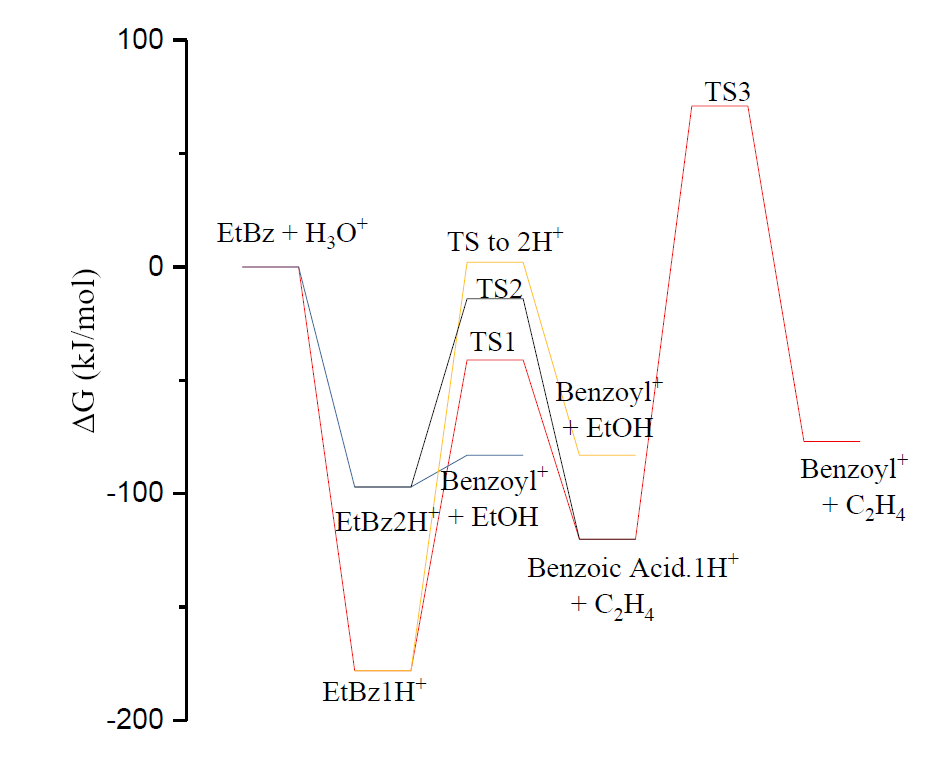
\includegraphics[width=0.7\linewidth]{pics/cocaine-chapter/etbz_deltag.png}
\caption{$\Delta$G for the various reactions of H$_3$O$^+$ with EtBz. Note that the neutral water has been omitted from the captions.}
\label{fig:etbz_deltag}
\end{figure}








% this is mine
Similarly to the MeBz case, other fragment ions are found at high \textit{E/N}, like
protonated benzene (C$_6$H$_7^+$) at \textit{m/z} 79 resulting from the loss of  CO$_2$ from BzAcidH$^+$. 
%
Although its formation is exergonic, it is thought to have a transition state similar to that in MeBzH$^+$ which can only be exceeded through collision-induced dissociation.
%
C$_6$H$_5^+$ at \textit{m/z} 77 (loss of H$_2$ from protonated benzene), 
C$_4$H$_3^+$ at \textit{m/z} 51 (loss of CH$_2$ from \textit{m/z} 77) in normal conditions and
the cluster of protonated ethyl benzoate with water at \textit{m/z} 169, this one in humid conditions, at low \textit{E/N} were also observed.














\subsubsection{Isopropyl benzoate}
Isopropyl benzoate is a key piece in this study because it resembles the benzoate moiety in the cocaine molecule, which is attached to two carbons. 
%
Similarly to MeBz and EtBz, iPrBz can undergo proton transfer from H$_3$O$^+$ and (H$_2$O)H$_3$O$^+$ but not from higher order water cluster ions, with iPrBzH$^+$ being the result of  proton transfer from (H$_2$O)H$_3$O$^+$ because, as it is explained below, proton transfer from H$_3$O$^+$ results in fragmentation.
%
The product ion intensities as a function of the drift voltage and the reduced electric field for the reaction of iPrBz with (H$_2$O)$_n$H$_3$O$^+$ (n = 0, 1) are given in \autoref{fig:iPrBzEN} and the energetics for the formation of the main product ions resulting from this reaction are provided in \autoref{tb:iprbz2}.


\begin{figure}[htbp]
\centering
\sidesubfloat[]{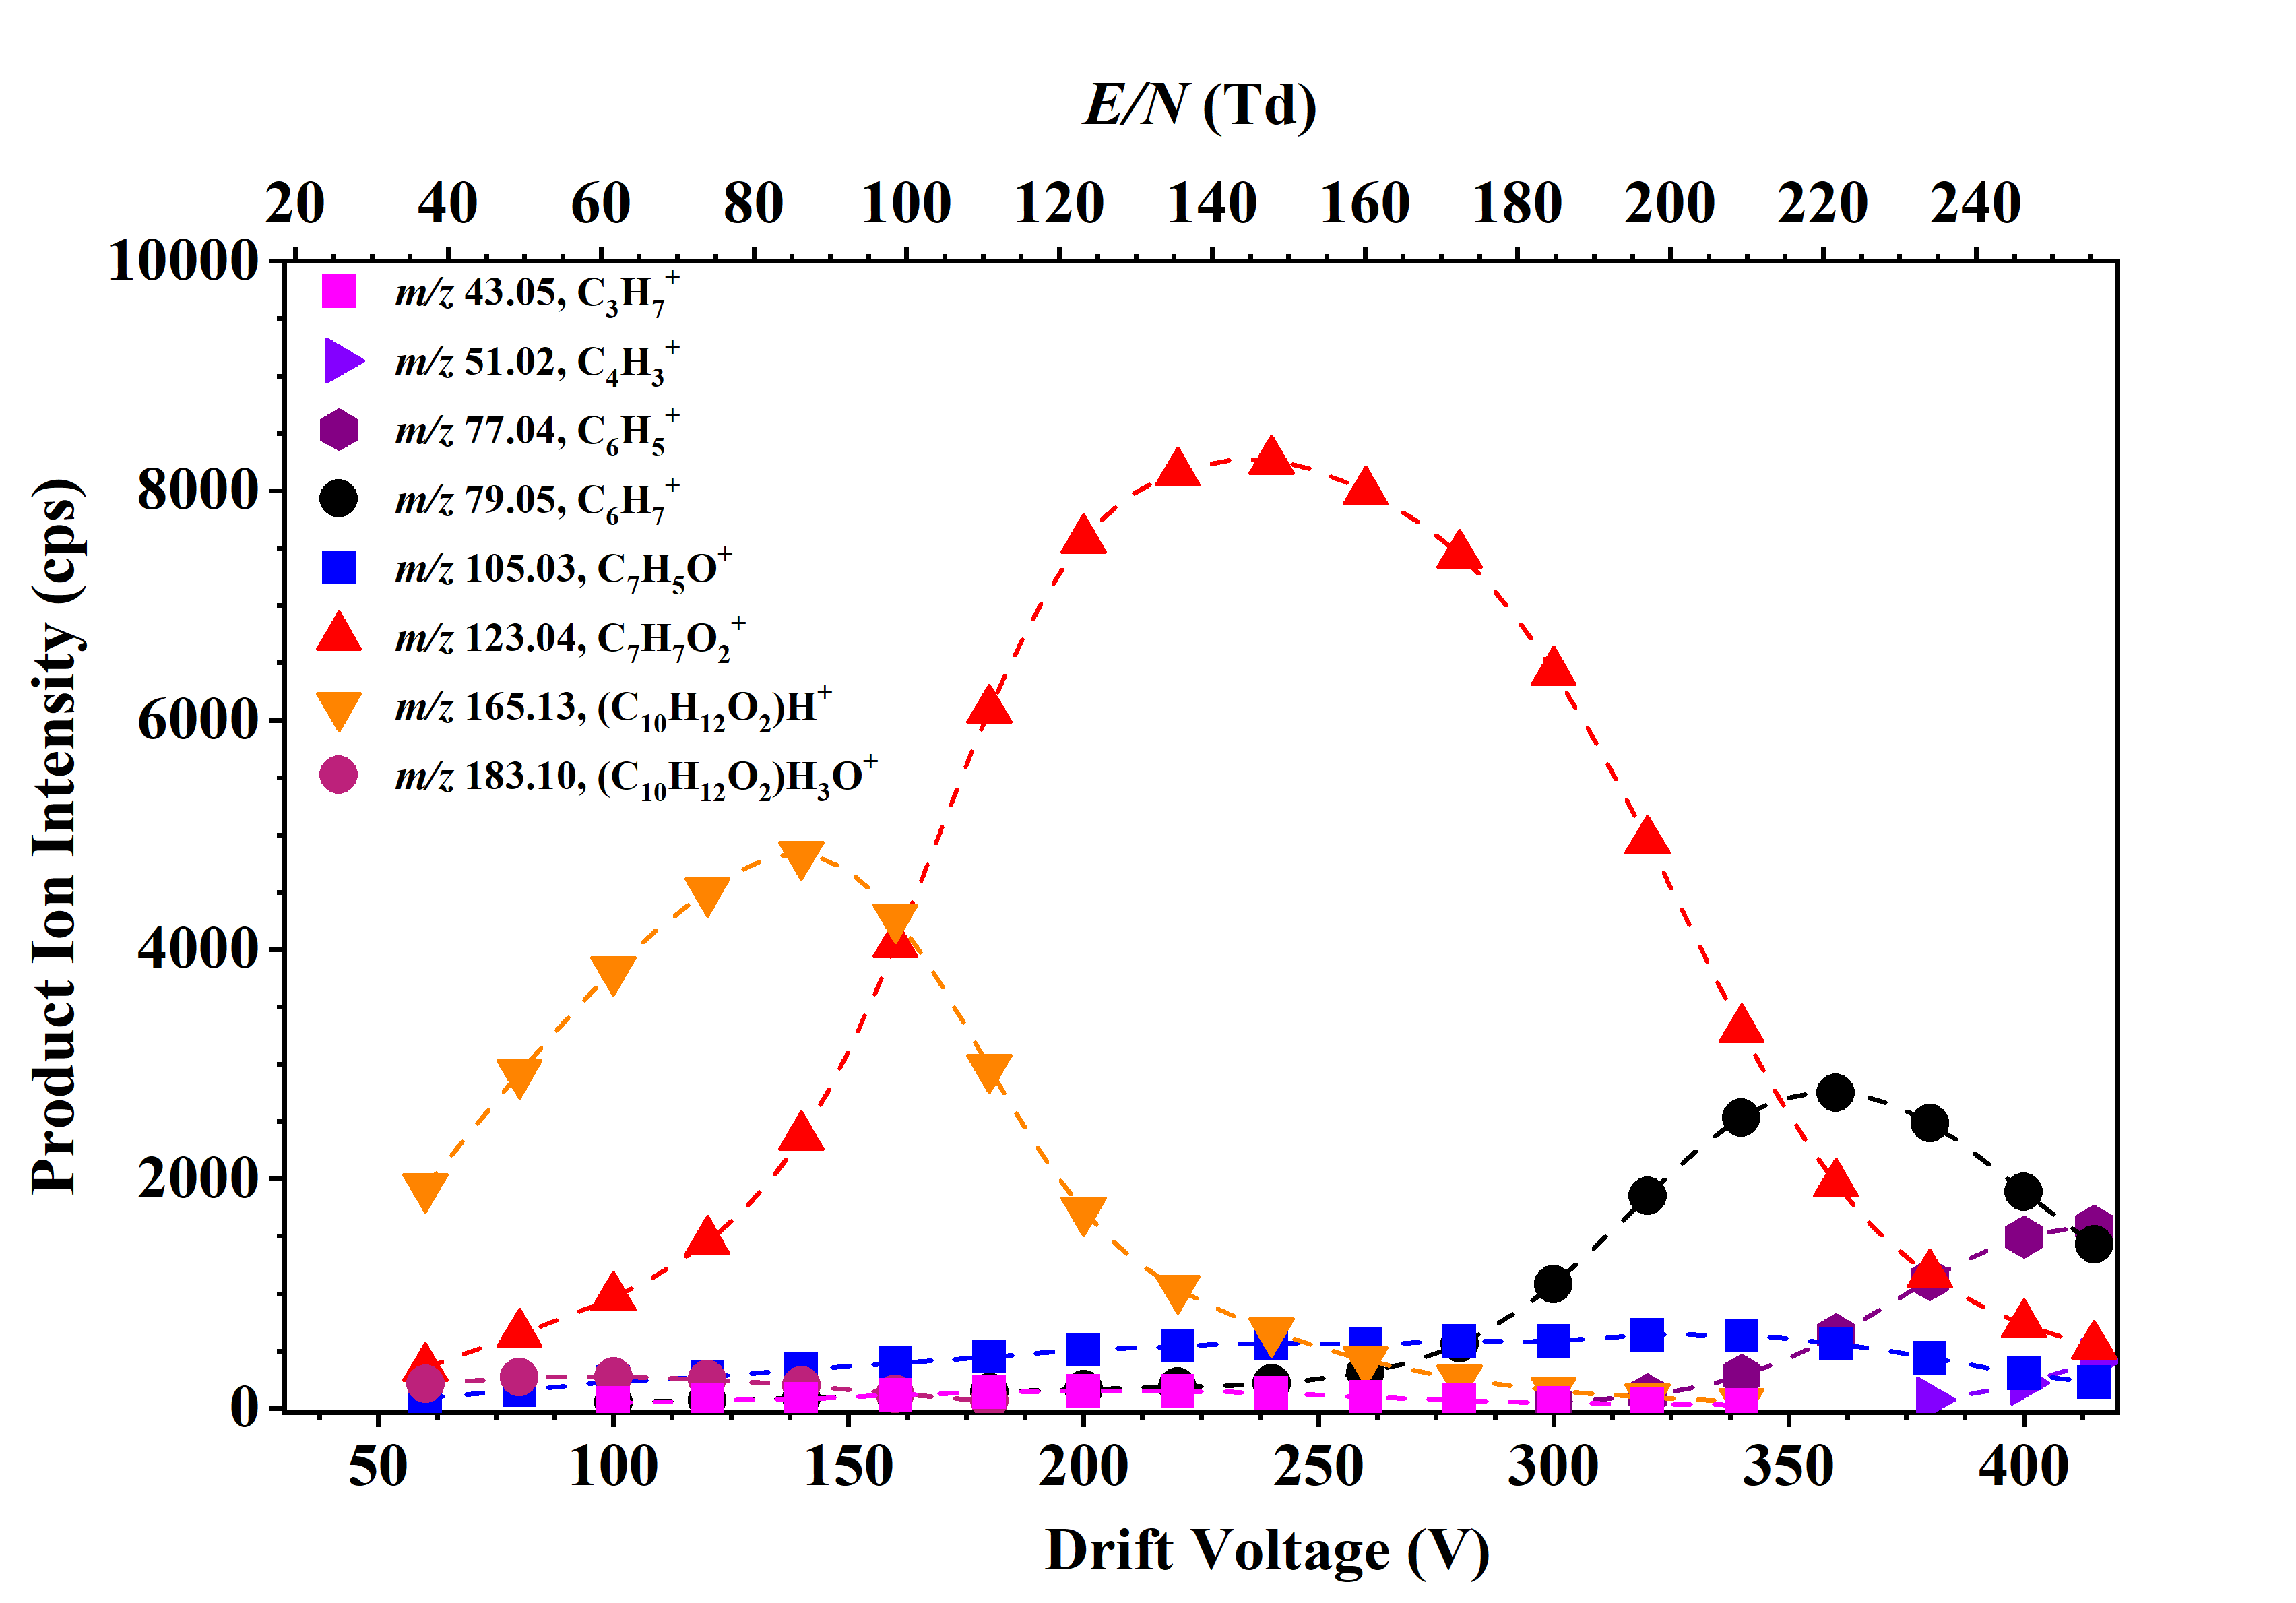
\includegraphics[width=0.8\linewidth]{pics/cocaine-chapter/iPrBz-cps3.png}}\\
\sidesubfloat[]{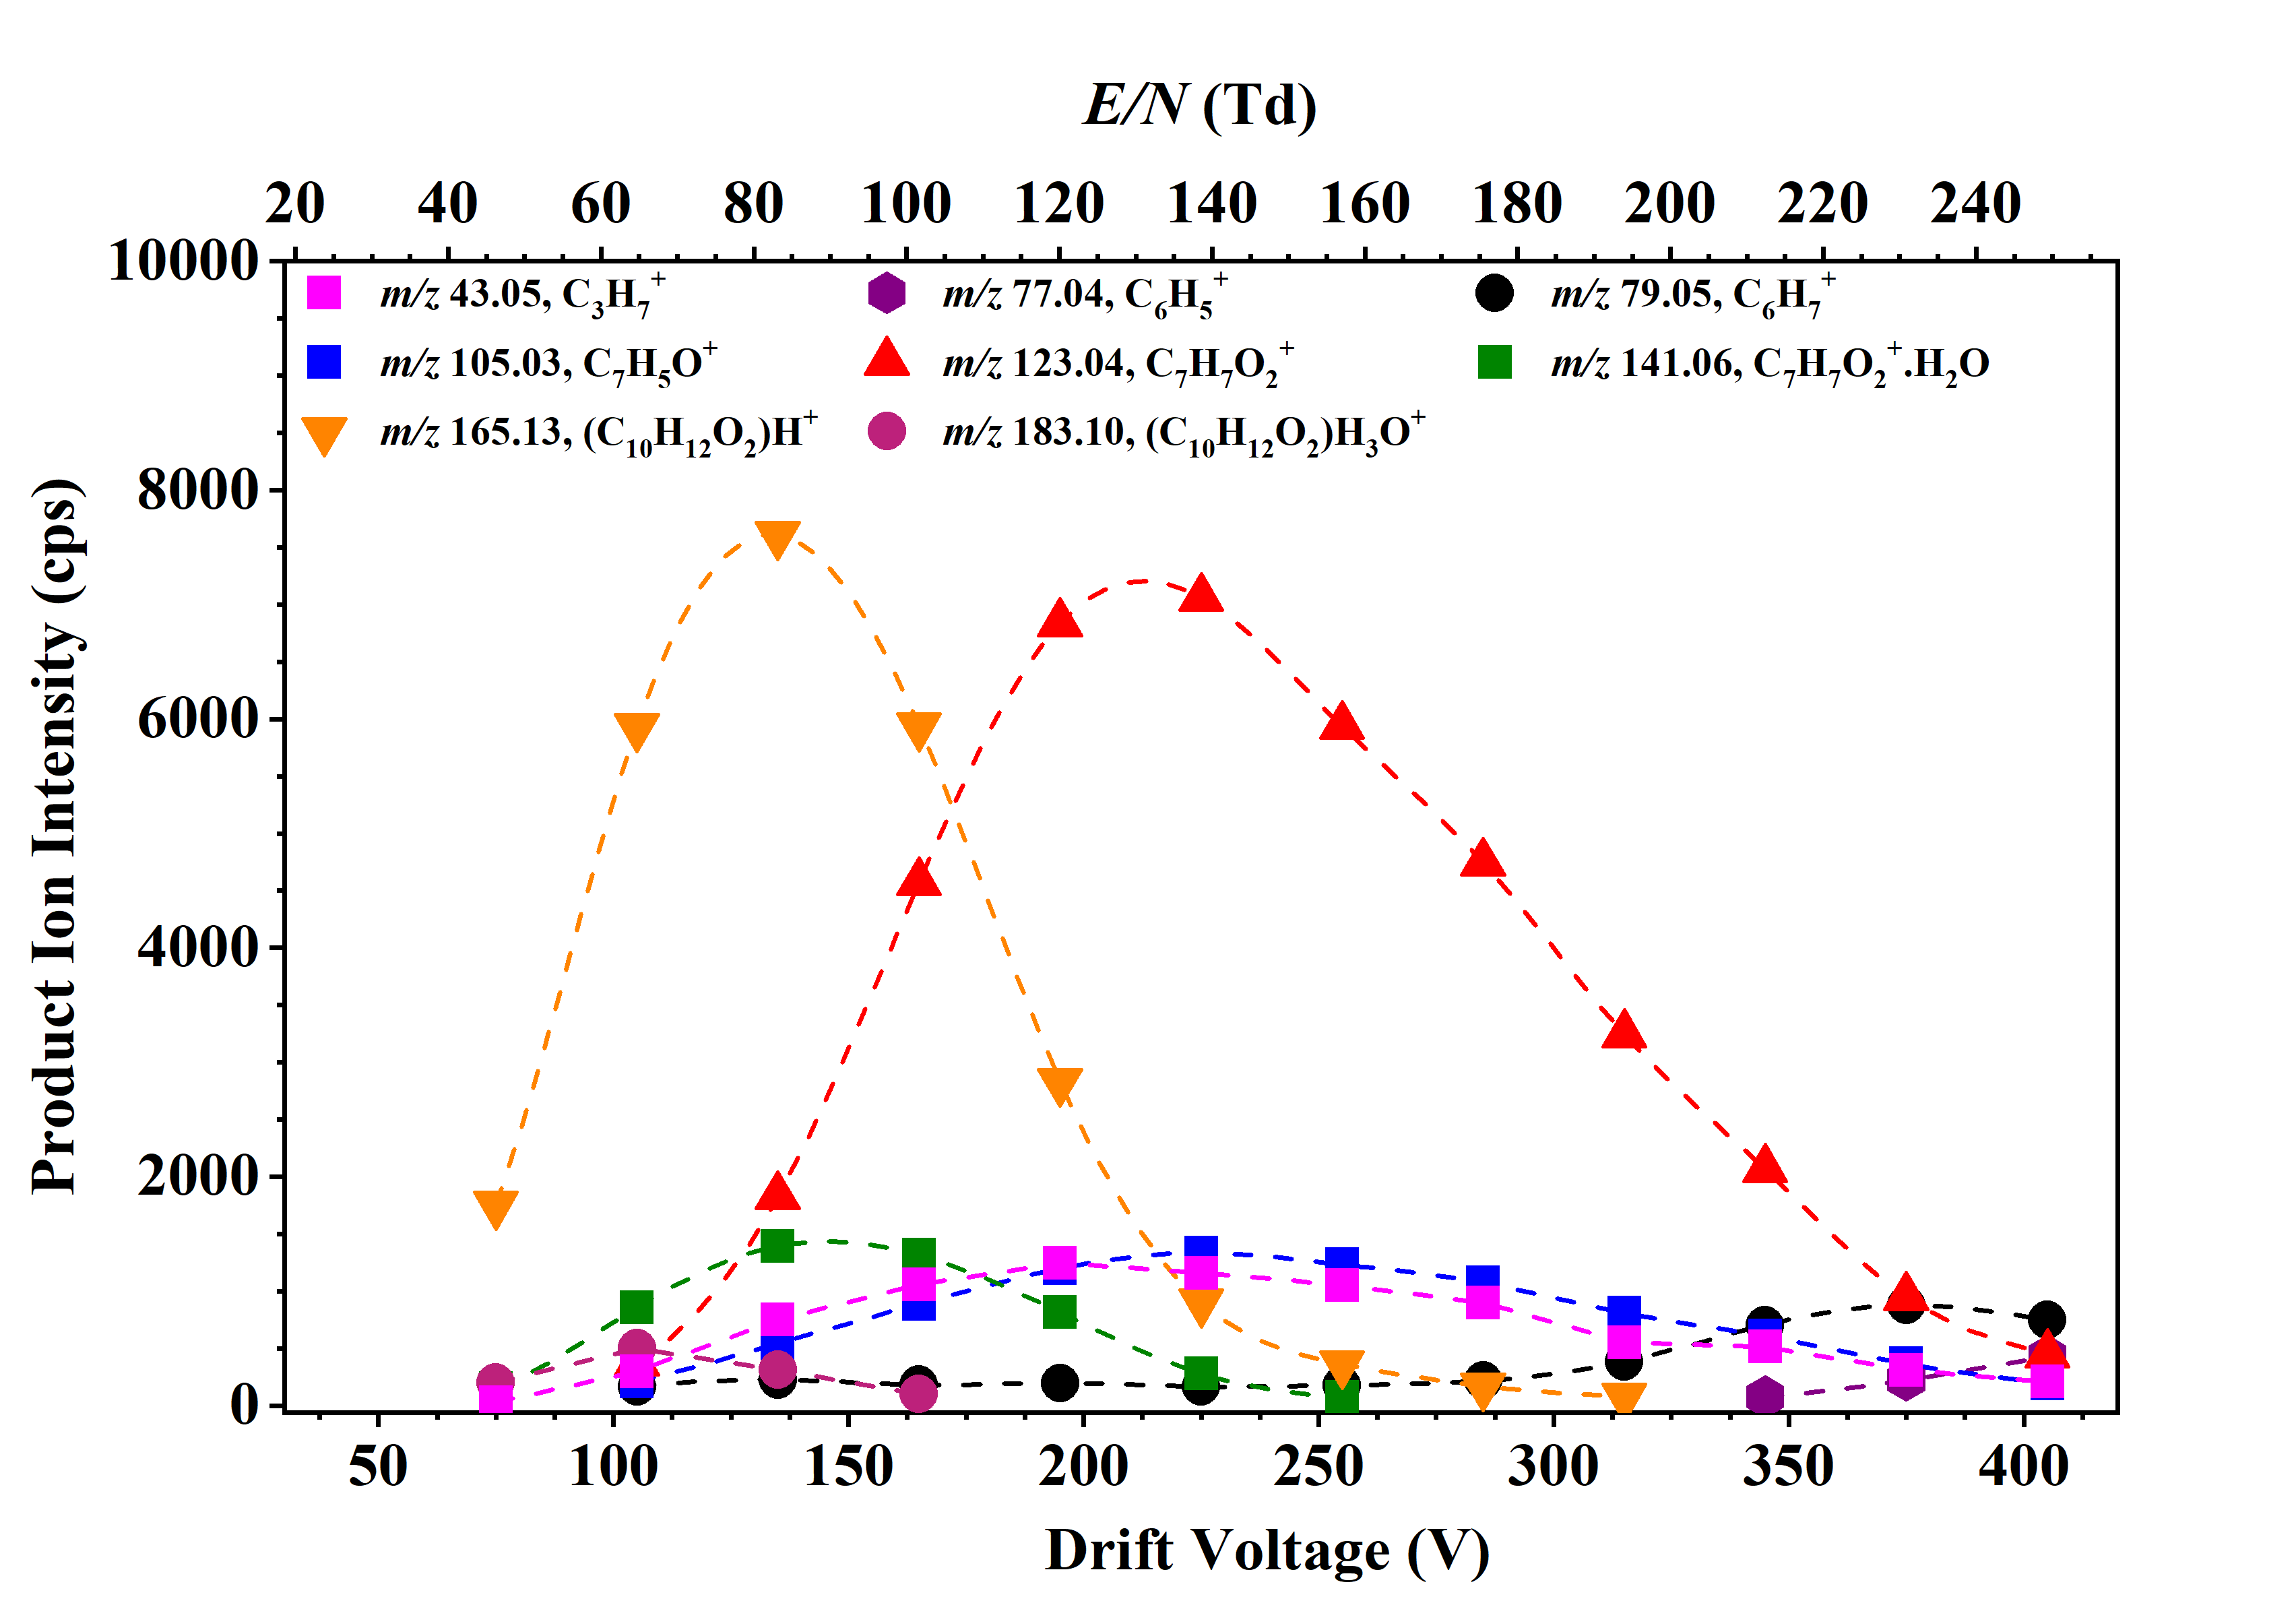
\includegraphics[width=0.8\linewidth]{pics/cocaine-chapter/humid/iPrBz-cps.png}}
\caption{Product ion signal intensities in counts per second of the product ions resulting from reactions of the H$_3$O$^+$.(H$_2$O)$_n$ (n = 0, 1) with isopropyl benzoate as a function of the drift voltage and the reduced electric field in (a) normal and (b) humid conditions.} 
\label{fig:iPrBzEN}
\end{figure}


\begin{table}[htbp]
\centering
\caption{Energetics relative to isopropyl benzoate and H$_3$O$^+$ and, in brackets, to isopropyl benzoate and (H$_2$O)H$_3$O$^+$. }
\label{tb:iprbz2}
\begin{tabular}{lccc}
\toprule
\textbf{Reaction or transition state}	&\textbf{\textit{m/z} } &\textbf{$\Delta$H$_{298}$} &\textbf{$\Delta$G$_{298}$}\\
& &	\textbf{(kJ/mol)} &\textbf{(kJ/mol)} \\  \toprule
iPrBz1H$^+$        & 165 & -176 (-18) & -177 (-53) \\ \midrule
iPrBz2H$^+$        & 165 & -102 (+56) & -107 (+17) \\ \midrule
TS 1H$^+$ to 2H$^+$   &  & -24 (+134) & -25 (+99) \\ \midrule
Benzoyl$^+$ + iPrOH & 105 & -45 (+113) & -99 (+25) \\ \midrule
Benzoic acid + iPr$^+$ & 43 & -35 (+123) & -91 (+33) \\ \midrule
TS1 for loss of propene from 1H$^+$ &  & -105 (+53) & -115 (+9) \\ \midrule
Benzoic acidH$^+$ + C$_3$H$_6$ & 123 & -84 (+74) & -137 (-13) \\ \midrule
BenzeneH$^+$ + C$_3$H$_6$ + CO$_2$ & 79 & -52 (+106) & -151 (-27) \\
\bottomrule
\end{tabular}
\end{table}




The product ion counts may indicate that the fragmentation pathways of iPrBz are similar to those of EtBz but the energetics show that these are actually quite different.
%
BzAcidH$^+$ is still the major fragment ion, in this case becoming dominant at a lower \textit{E/N} compared to EtBz (i.e. at ca. 100 Td for both the normal and humid experiments), although protonated benzene at \textit{m/z} 79 is the dominant ion at the higher end of the \textit{E/N} range.
%
Benzoyl$^+$ at \textit{m/z} 105 is found over the same range it was found for EtBz.
%
Furthermore, a new ion at \textit{m/z} 43, tentatively assigned to isopropyl radical (iPr$^+$, C$_3$H$_7^+$), is also found with a comparable abundance of that of benzoyl$^+$ in  humid conditions but only traces were observed in the measurements in normal conditions.
%
Other product ions that were observed are
the cluster with water of protonated benzoic acid and protonated isopropyl benzoate at \textit{m/z} 141 and \textit{m/z} 183, respectively, at low \textit{E/N}, and C$_6$H$^+_5$ at m/z 77 (loss of H$_2$ from protonated benzene) and  C$_4$H$^+_3$ at \textit{m/z} 51 (loss of CH$_2$ from \textit{m/z} 77) at high \textit{E/N}.


%The fragmentation of iPrBz is remarkably different from that of EtBz. Whilst BzAcidH$^+$ is still the major fragment ion it is now the dominant ion and occurs at much lower \textit{E/N}. 
%The benzoyl$^+$ fragment ion occurs over a similar range of \textit{E/N} as was observed with EtBz and a new fragment ion with \textit{m/z} 43, the iPr$^+$ cation is observed over a similar range of \textit{E/N}  and with a similar intensity. 
%The PA and GB are 861 and 831 kJ mol$^{-1}$ respectively and as with EtBz protonation will occur by H$_3$O$^+$ and (H$_2$O)H$_3$O$^+$ but not by higher clusters, but as will be seen the iPrBzH$^+$ must be formed from (H$_2$O)H$_3$O$^+$. 


As with MeBz and EtBz, the loss of an alcohol needs the proton to be on O2.
%
For iPrBz, loss of isopropyl alcohol (iPrOH) from iPrBz2H$^+$ yields benzoyl$^+$, but fragmentation of iPrBz2H$^+$ can also result in iPr$^+$. 
%
This can be illustrated with the structures in \autoref{fig:iprbz_ts}.
%
The length of the C1-O and C2-O bonds in EtBz2H$^+$ are 1.74 and  1.50   \r{A}, respectively.
%
The length of these for iPrBz2H$^+$ are  1.62 and 1.57  \r{A}.
%
The C1-O bond in iPrBz2H$^+$ is longer that the equivalent in the iPrOH molecule, which is 1.44 \r{A}.
%
This longer bond allows the iPr$^+$ ion to be formed.
%
The formation of both fragment ions of iPrBz2H$^+$ (i.e. iPr$^+$ and benzoyl$^+$ from the loss of iPrOH) have similar energetics and both are barrierless (as shown in \autoref{fig:iprbz_deltag}).
%
There are however two questions that can be asked at this point:
%
(i) why are there such differences in the ion signals of \textit{m/z} 43 and \textit{m/z} 105 in normal conditions when they have similar intensities (as expected) in the humid measurements?
And, considering that  iPr$^+$ resembles the fragment with \textit{m/z} 182 in the benzoate moiety, (ii)  why is iPr$^+$ so low compared to \textit{m/z} 182 in the cocaine measurements?
%
While the first question remains unanswered for now, there are two possible explanations for the second one.
%
In first place, ions with bigger \textit{m/z} are transported more efficiently through the different stages of the PTR-ToF-MS.
%
This is the reason transmission coefficients are often used to account for ion losses of lower \textit{m/z} ions.
%
The other reason could be related to the fact that iPrBz was measured through headspace analysis while the TDU was used for studying cocaine, potentially decomposing some of the sample which then gets ionised in the drift tube.
%
However it is unlikely that the latter is the reason because the product ion with \textit{m/z} 182 in cocaine presents a comparable branching percentage to that reported by \citeauthor{Agarwal2011} (i.e. ca. 15\% of the total product ion counts at 120 Td)  \cite{Agarwal2011}.%, who studied the detection of different drugs through headspace analysis \cite{Agarwal2011}.






%iPrBz2H$^+$ is the precursor to both the loss of iPrOH and iPr+.
%To see why both pathways occur it is instructive to compare the structures of EtBz2H$^+$ and iPrBz2H$^+$ in \autoref{fig:iprbz_ts}.
%
%In EtBz2H$^+$ the C-O bond of the potential alcohol compares well with the 1.43 \r{A} in EtOH (or 1.45 in EtBz) with a concomitant lengthening of the carbonyl oxygen bond. In iPrBz2H$^+$ the C-O of the potential alcohol is less well developed in comparison with the C-O bond in iPrOH 1.44 \r{A} leading to a shortening of the carbonyl oxygen bond. A consequence of the long C-O bond of the potential iPrOH is the potential formation of the iPr$^+$ cation. As the energies for both of the dissociation channels of iPrBz2H$^+$ are virtually identical, and both dissociation processes are barrierless as confirmed by relaxed scans, it is not surprising that both are followed to a similar degree. 
%"You will appreciate I now have a problem to explain why 43 has such a low intensity particularly as the formation of 182 in cocaine (the dominant fragment ion) has similar energetics. Moreover the similarity to the benzoate moiety of cocaine was the reason we investigated iPrBz – see earlier in this section". 

\begin{figure}[htbp]
\centering
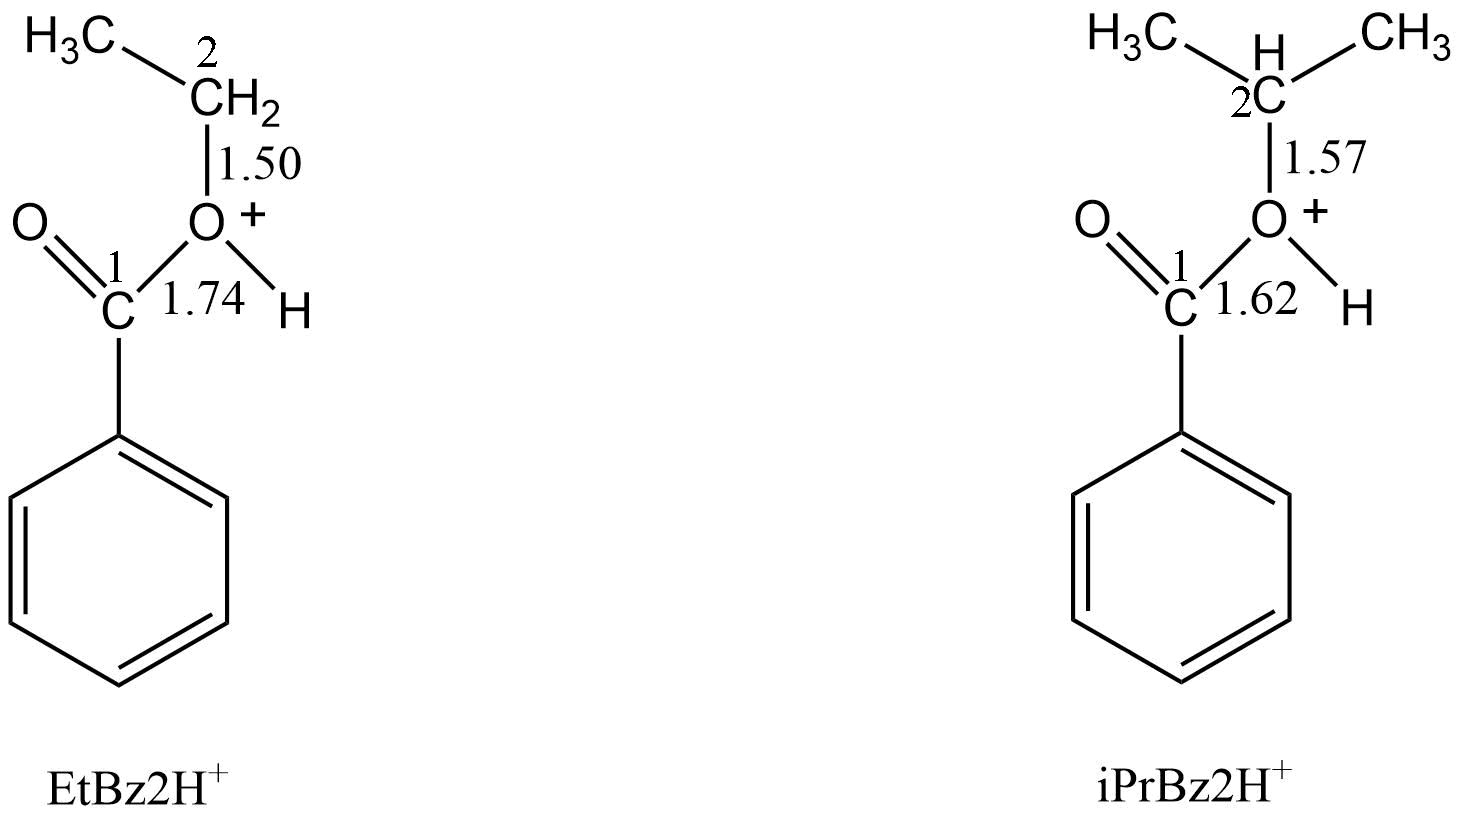
\includegraphics[width=0.5\linewidth]{pics/cocaine-chapter/iprbz_ts.png}
\caption{Structure of EtBz2H$^+$ and iPrBz2H$^+$.}
\label{fig:iprbz_ts}
\end{figure}



The plot of $\Delta$G as a function of the reaction coordinate in \autoref{fig:iprbz_deltag} indicate that protonation from H$_3$O$^+$ will readily result in fragmentation and hence any observed protonated iPrBz will  come from the reaction with (H$_2$O)H$_3$O$^+$ having the structure iPrBz1H$^+$.
%
That the dominant product is BzAcidH$^+$ indicates that whilst direct protonation of O2 can occur, protonation or the more basic O1 is more likely, probably influenced by dipolar attraction.
%
The difference in energy between iPrBz1H$^+$ and TS1 is only of 62 kJ mol$^{-1}$, while for EtBz this is 137 kJ mol$^{-1}$, which explains why BzAcidH$^+$ is observed at lower \textit{E/N} in iPrBz compared to EtBz.




%Inspection of the reaction coordinate in \autoref{fig:iprbz_deltag} shows that protonation by H$_3$O$^+$ will result in immediate fragmentation to all primary products thus any iPrBzH$^+$ observed results from protonation by (H$_2$O)H$_3$O$^+$ to yield iPrBz1H$^+$.

%The only significant dependence of a product ion upon \textit{E/N} is that of \textit{m/z} 141 BzAcidH$^+$H$_2$O.




\begin{figure}[htbp]
\centering
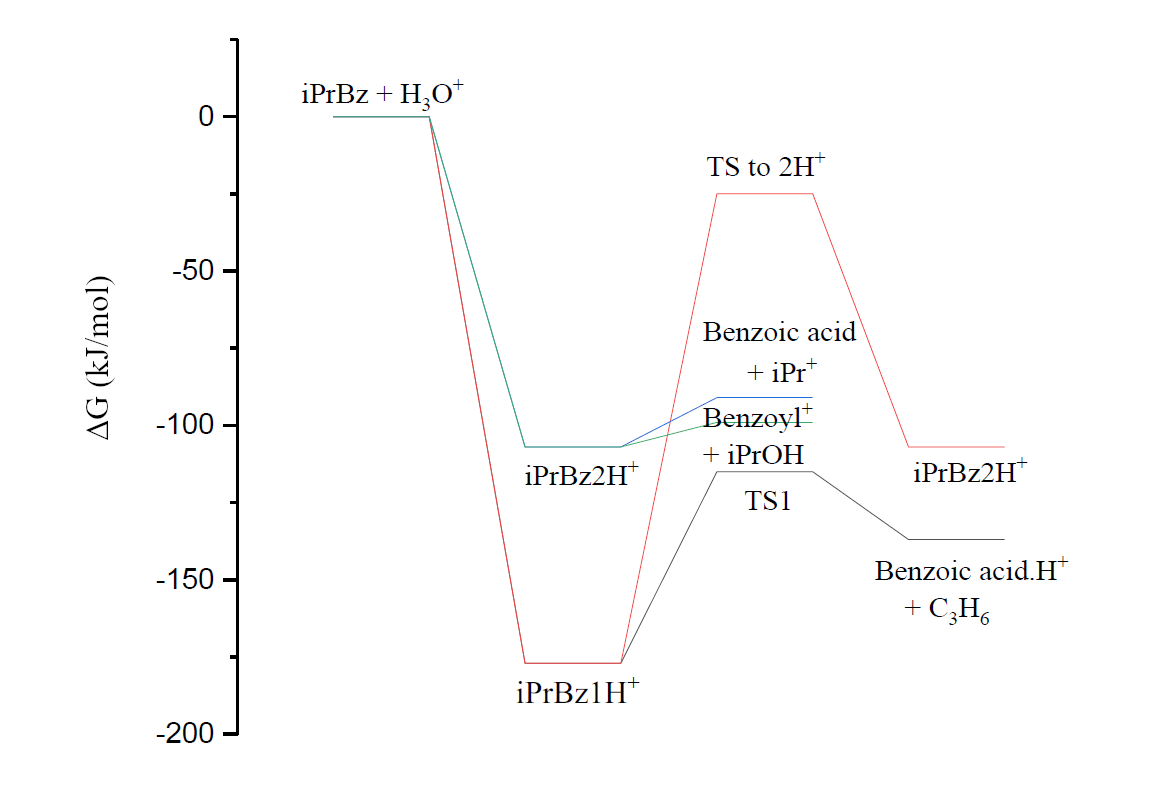
\includegraphics[width=0.7\linewidth]{pics/cocaine-chapter/iprbz_deltag.png}
\caption{$\Delta$G for the various reactions of H$_3$O$^+$ with iPrBz. Note that the neutral water has been omitted from the captions.}
\label{fig:iprbz_deltag}
\end{figure}










\subsubsection{Benzoic acid}
Protonated cocaine losses benzoic acid to give the ion with \textit{m/z} 182, which is the major fragment ion of cocaine.
%
For this reason, benzoic acid was included in this study.
%
%Because of the possible formation of benzoic acidH$^+$ from benzoyl$^+$ and H$_2$O and vice versa, it was interesting to study benzoic acid in the PTRMS.
%
%
%
Similarly to the benzoate esters, BzAcid can undergo proton transfer from (H$_2$O)H$_3$O$^+$, to give BzAcid1H$^+$, and H$_3$O$^+$, to give either BzAcid1H$^+$ or BzAcid2H$^+$, although the latter readily fragments to benzoyl$^+$ + H$_2$O. 
%
The product ion intensities as a function of the drift voltage and the reduced electric field for the reaction of BzAcid with (H$_2$O)$_n$H$_3$O$^+$ (n = 0, 1) are given in \autoref{fig:bzacidEN} and the energetics for the formation of the main product ions resulting from this reaction are provided in \autoref{tb:bzacid2}.

\begin{figure}[htbp]
\centering
\sidesubfloat[]{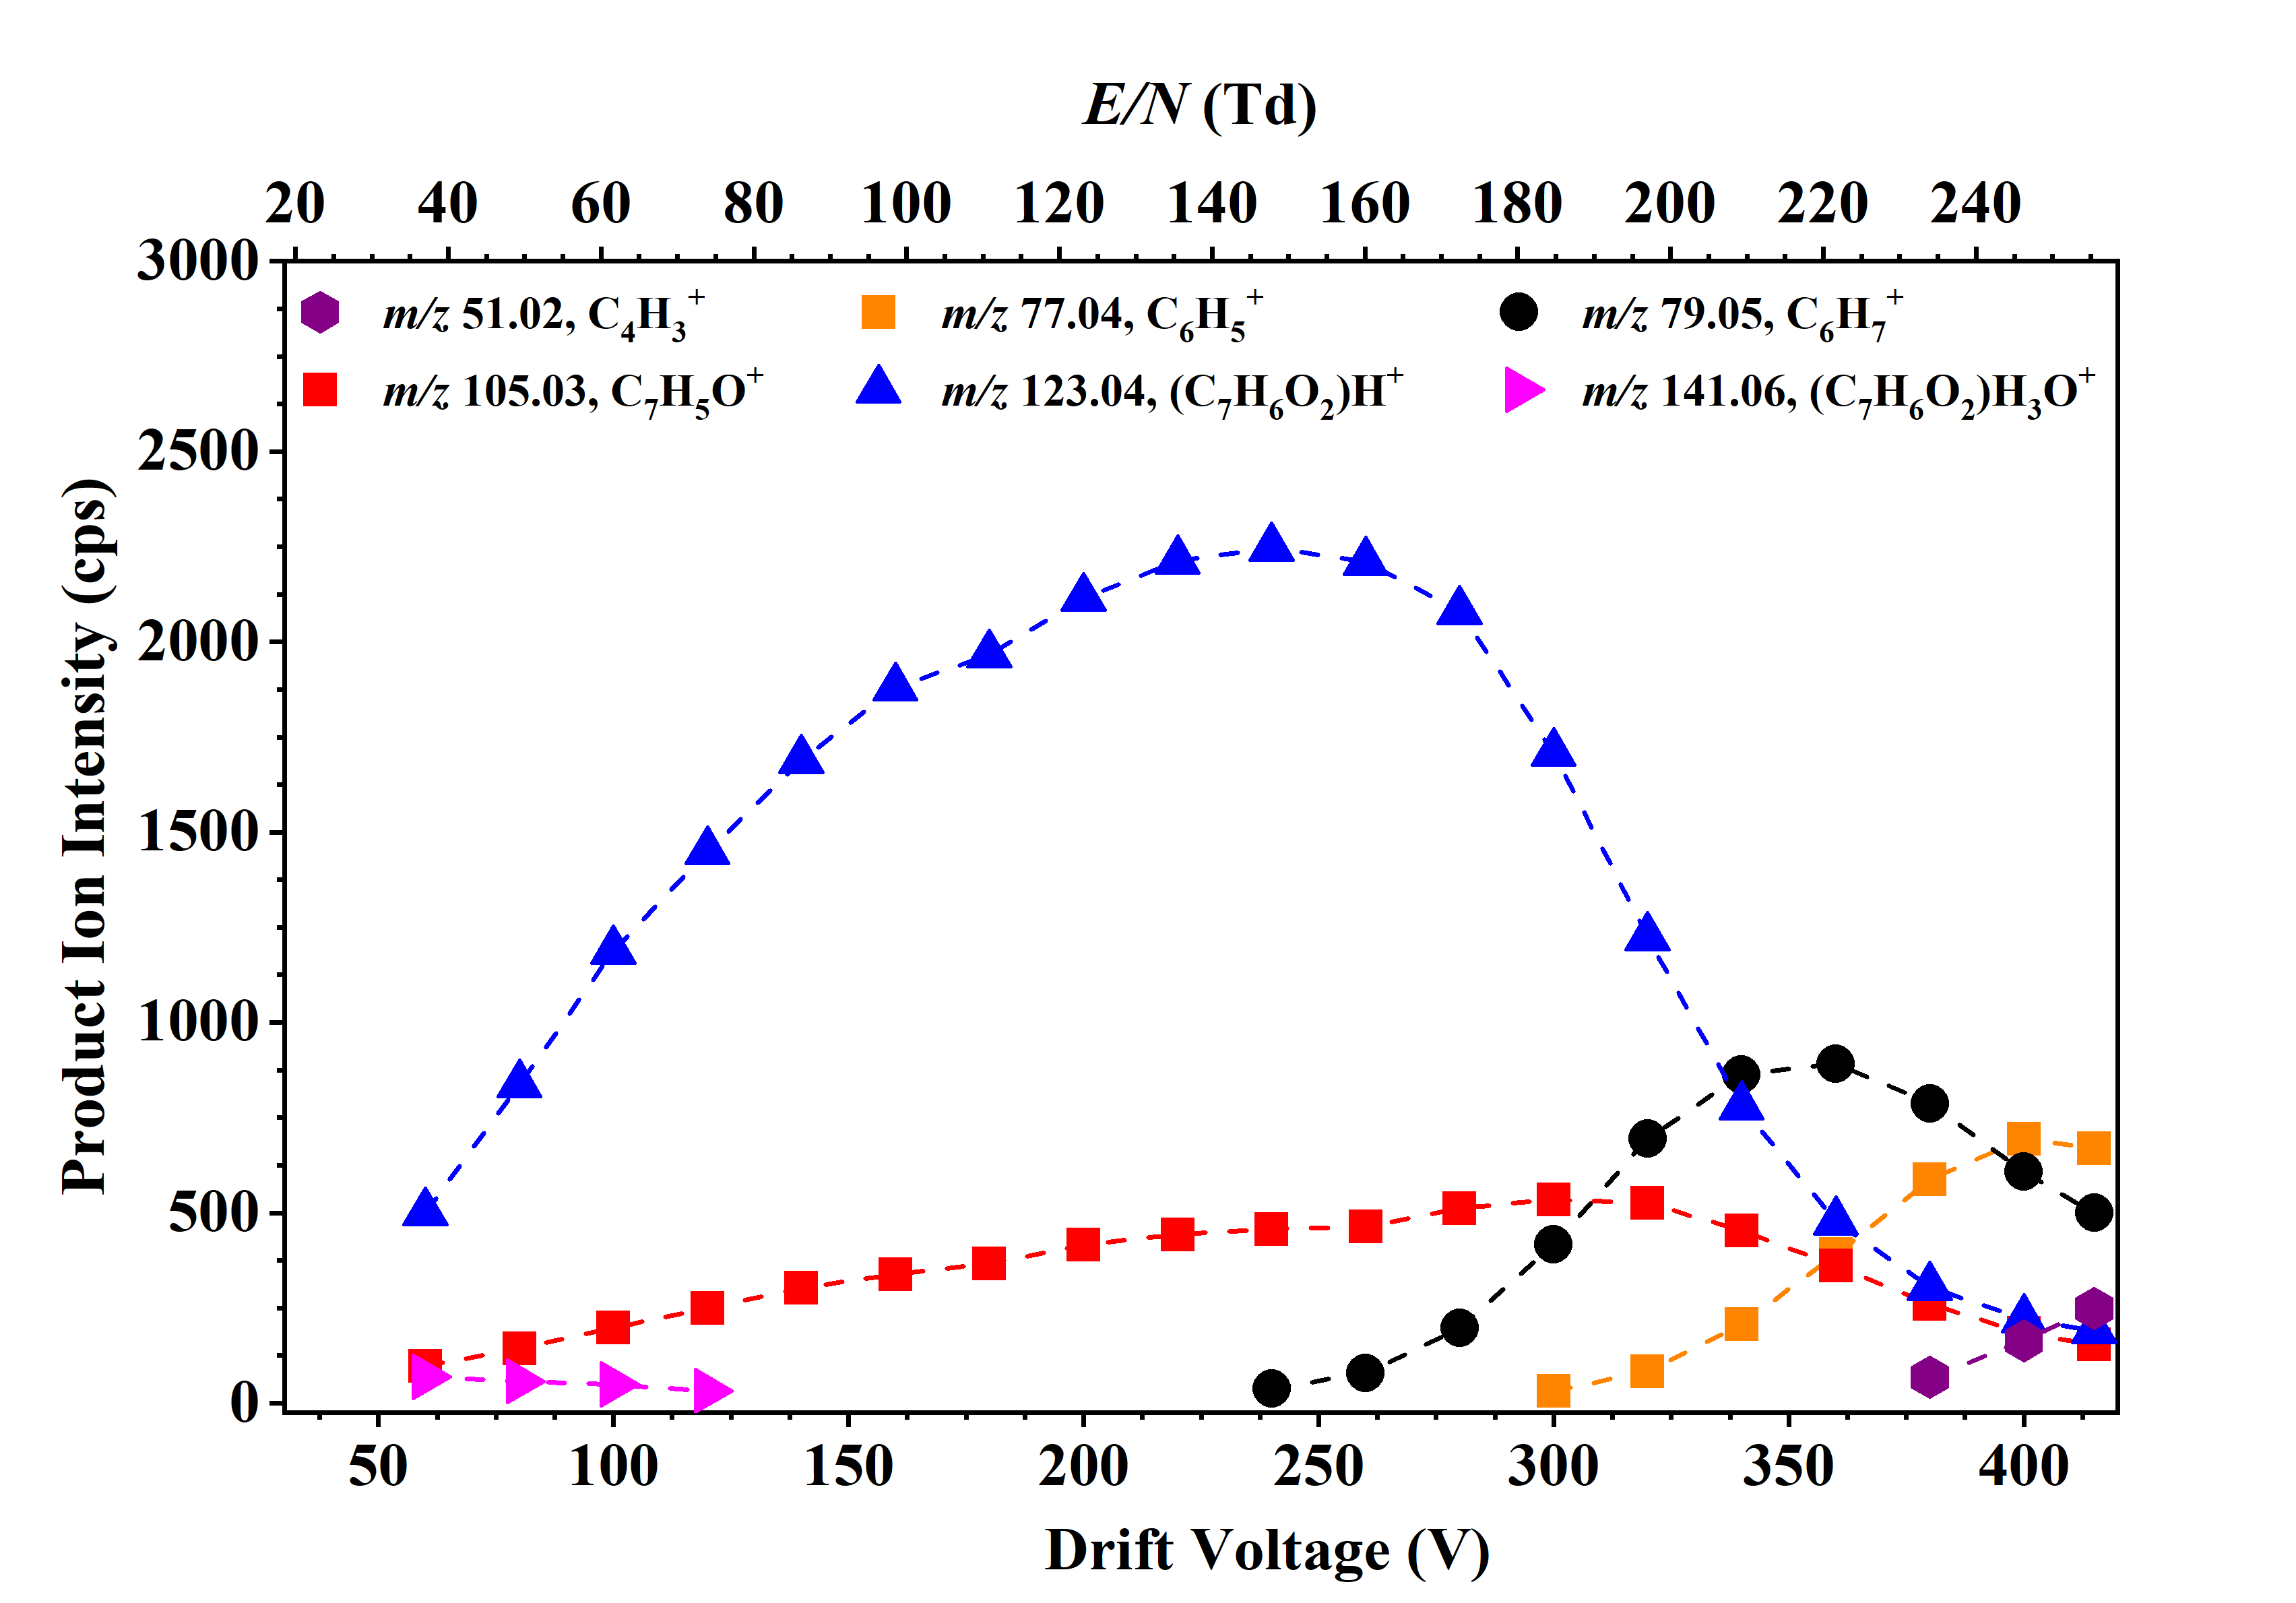
\includegraphics[width=0.8\linewidth]{pics/cocaine-chapter/BzAcid-cps.png}}\\
\sidesubfloat[]{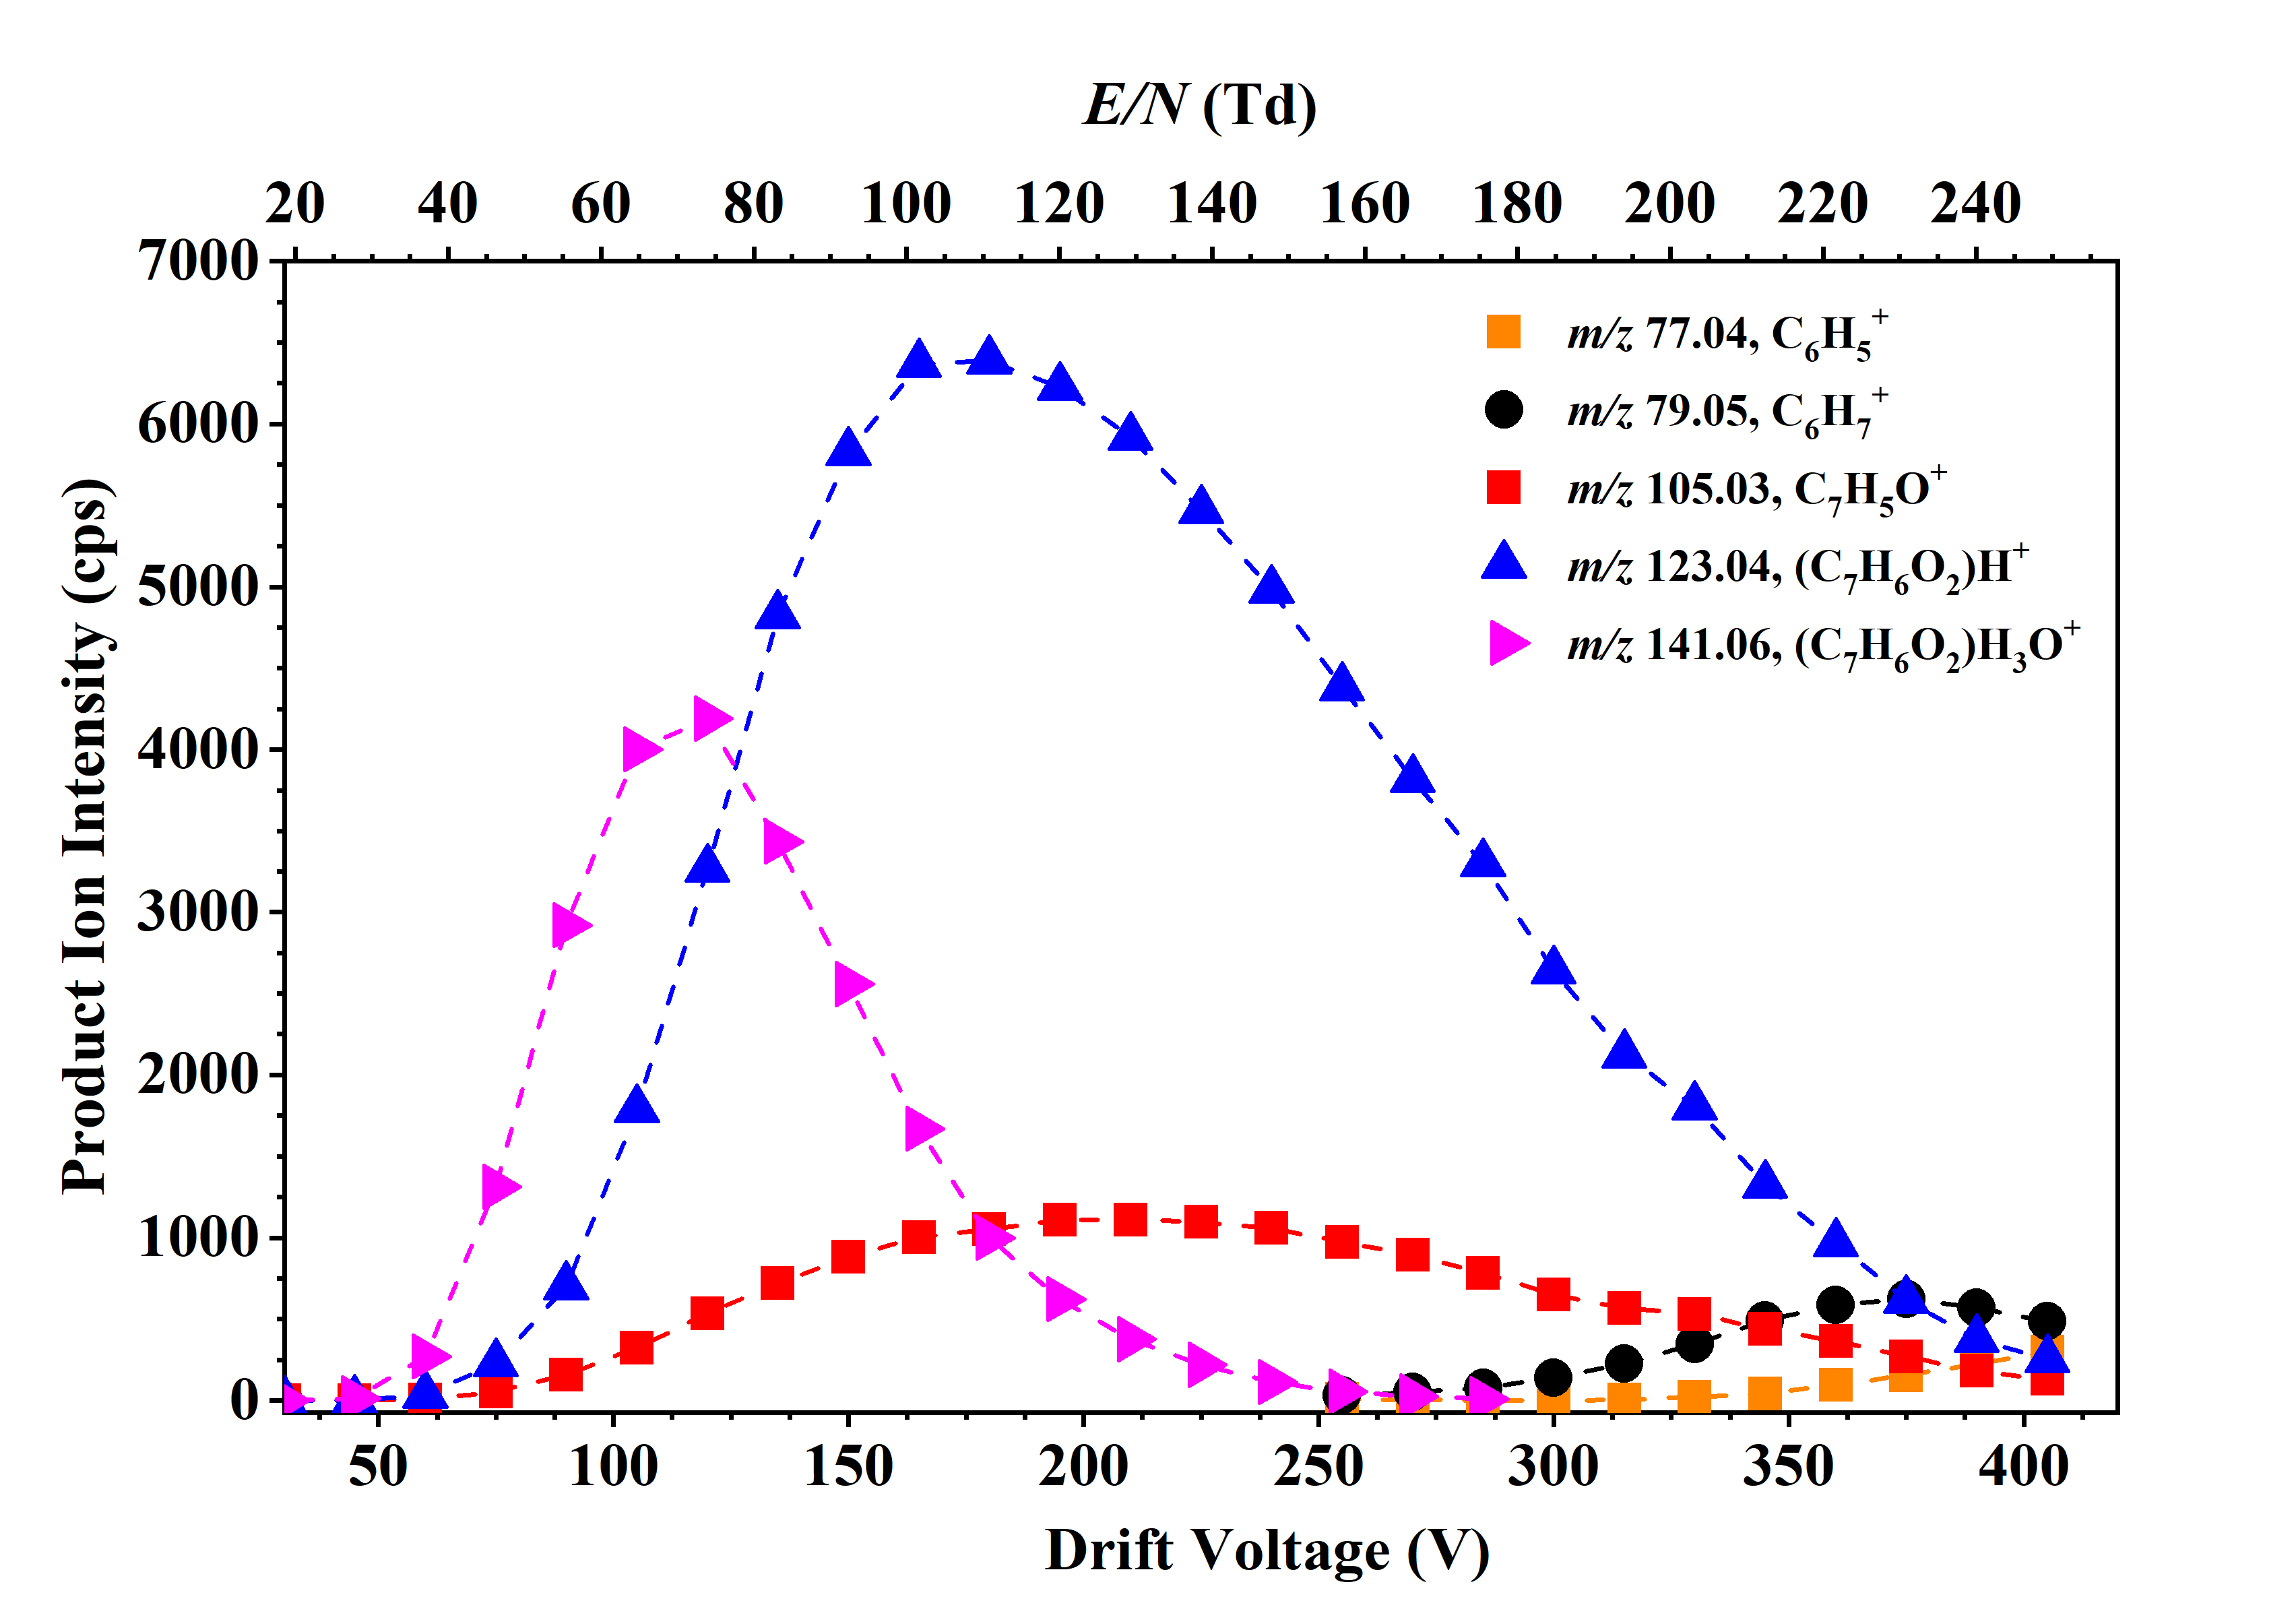
\includegraphics[width=0.8\linewidth]{pics/cocaine-chapter/humid/BzAcid-cps.png}}
\caption{Product ion signal intensities in counts per second of the product ions resulting from reactions of the H$_3$O$^+$.(H$_2$O)$_n$ (n = 0, 1) with benzoic acid as a function of the drift voltage and the reduced electric field in (a) normal and (b) humid conditions.} 
\label{fig:bzacidEN}
\end{figure}

\begin{table}[htbp]
\centering
\caption{Energetics relative to benzoic acid and H$_3$O$^+$ and, in brackets, to benzoic acid and (H$_2$O)H$_3$O$^+$.}
\label{tb:bzacid2}
\begin{tabular}{lccc}
\toprule
\textbf{Reaction or transition state}	&\textbf{\textit{m/z} } &\textbf{$\Delta$H$_{298}$} &\textbf{$\Delta$G$_{298}$}\\
& &	\textbf{(kJ/mol)} &\textbf{(kJ/mol)} \\  \toprule
BzAcid1H$^+$ & 123 & -128 (+30) & -130 (-6) \\ \midrule
BzAcid2H$^+$ & 123 & -40 (+118) & -88 (+36) \\ \midrule
TS 1H$^+$ to 2H$^+$ &  & +44 (+202) & +45 (+169) \\ \midrule
Benzoyl$^+$ + H$_2$O  & 105 & -83 (+75) & -100 (+24) \\ \midrule
BenzeneH$^+$ + CO$_2$ & 79 & -97 (-61) & -143 (-19) \\
\bottomrule
\end{tabular}
\end{table}

%\begin{figure}[htbp]
%\centering
%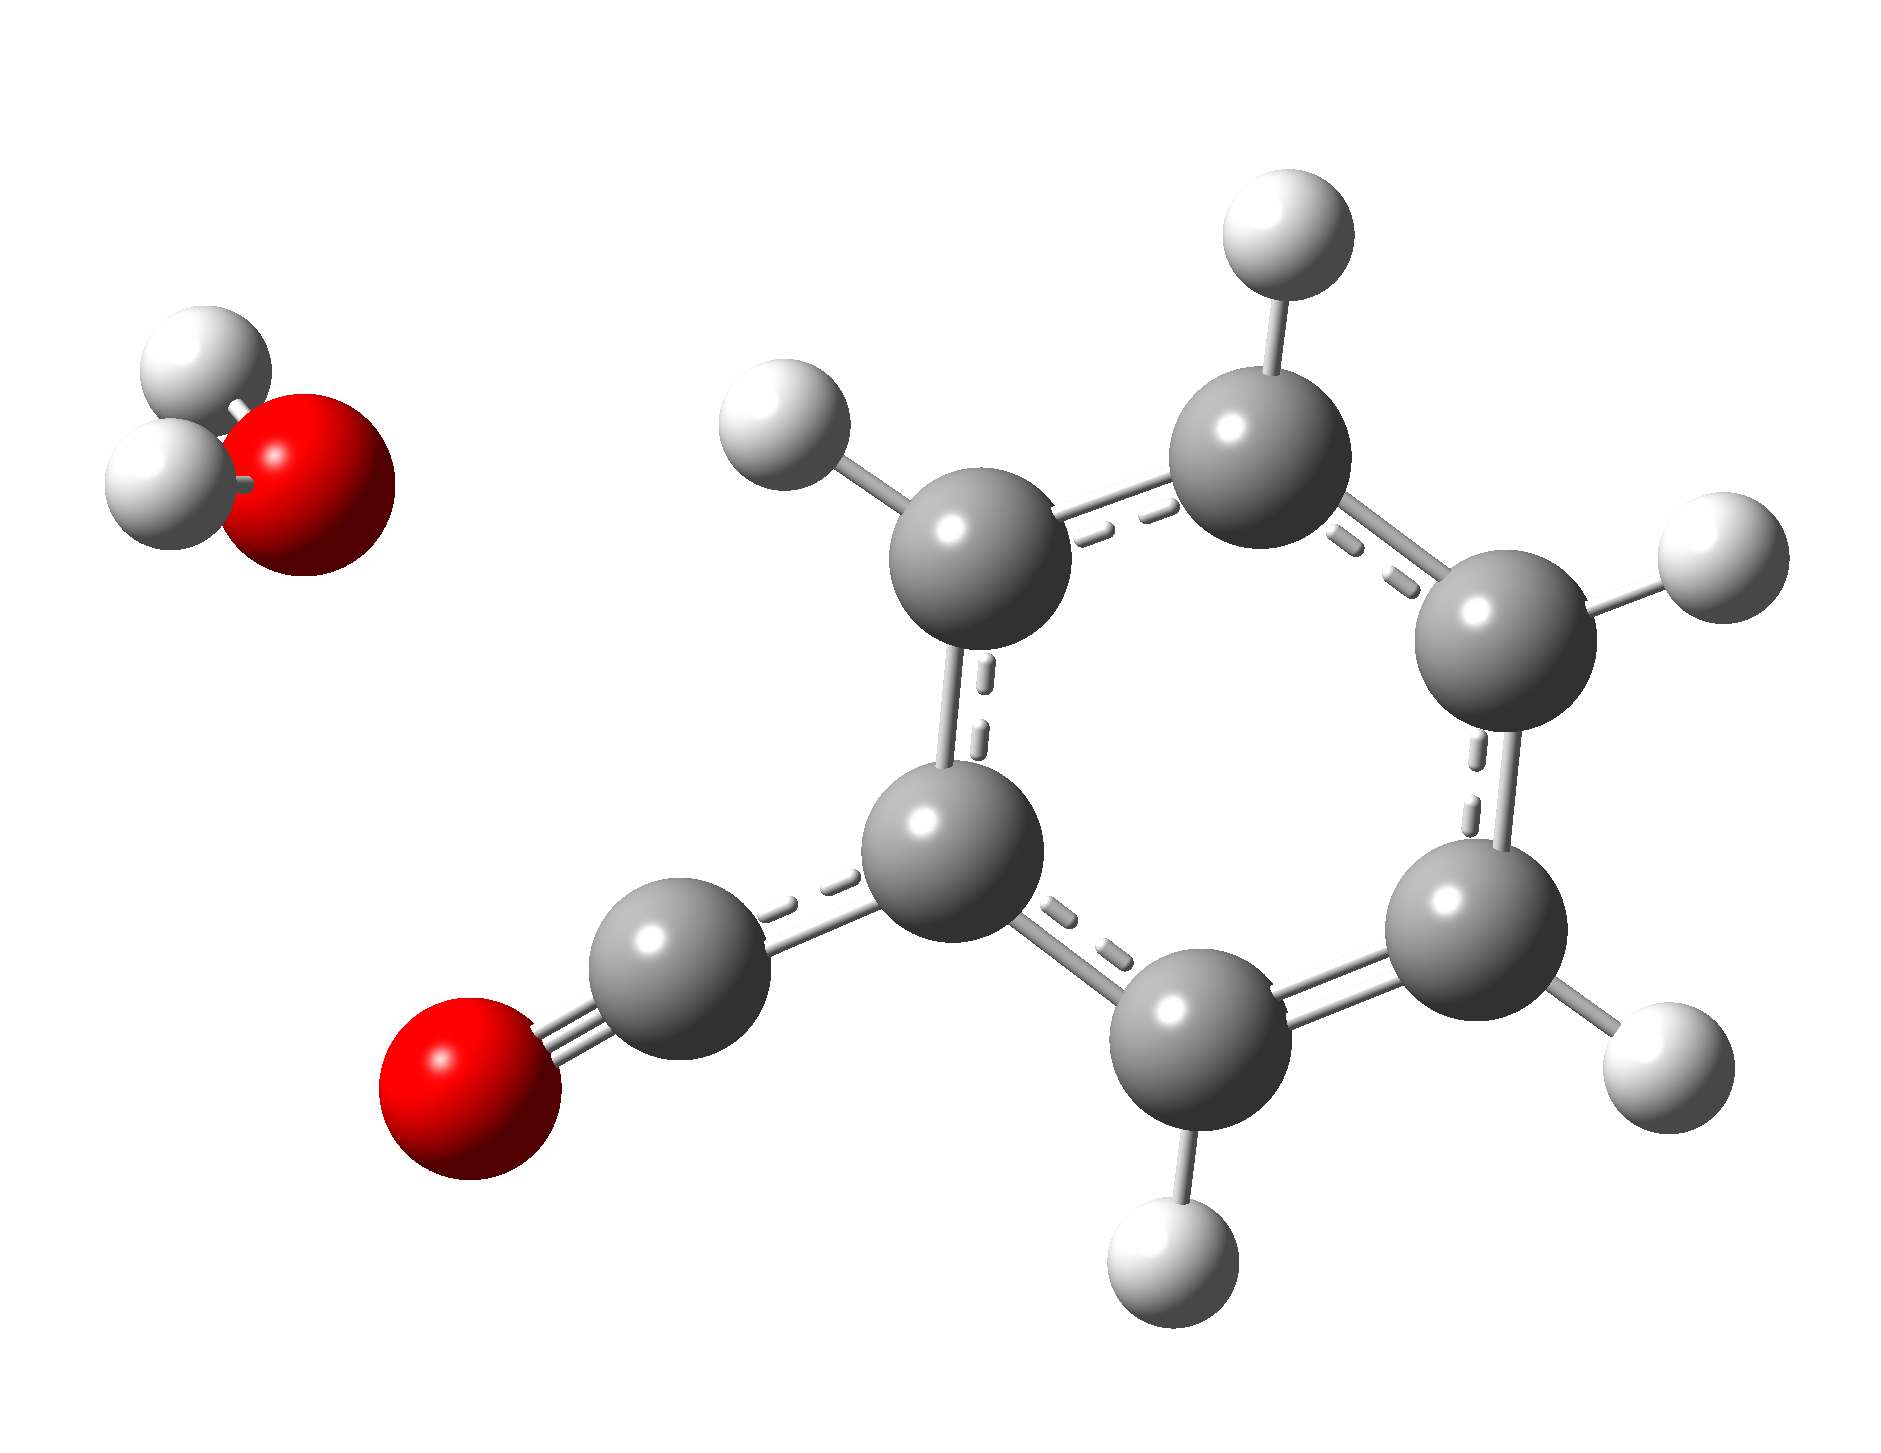
\includegraphics[width=0.4\linewidth]{pics/cocaine-chapter/bzacid_fragment.png}
%\caption{Structure of BzAcid2H$^+$.}
%\label{fig:bzacid_fragment}
%\end{figure}




For this compound, the protonated parent molecule at \textit{m/z} 123 is the dominant ion for most of the \textit{E/N} range, with protonated benzene and its loss of H$_2$ (i.e. \textit{m/z} 79 and \textit{m/z} 77) appearing at high \textit{E/N}, and the cluster of protonated BzAcid with water at low \textit{E/N} (more remarkable in humid conditions).
%
Like with the previous compounds, the formation of benzoyl$^+$ at \textit{m/z} 105 requires the proton to be on O2, to yield BzAcid2H$^+$ in this case, followed by the barrierless disociation of water.
%
Benzoyl$^+$ being produced at all reduced electric fields proves again that direct protonation of O2 occurs, because the TS 1H$^+$ to 2H$^+$ is endergonic and hence benzoyl$^+$ is not a product of the structure BzAcid1H$^+$.
%
When the PTR-MS results from BzAcid are compared to those from MeBz, EtBz and iPrBz  at low \textit{E/N}, it can be concluded that the formation of benzoyl$^+$ does not occur from fragmentation of protonated benzoic acid, but by direct protonation of the alkoxy oxygen O2 for each molecule.
%
Furthermore, \autoref{fig:bzacidEN} also proves that protonated benzene and its loss of H$_2$ are formed from protonated benzoic acid through collision-induced dissociation at high \textit{E/N}.



%The plot shows that whilst benzoyl$^+$ is formed over the same range of \textit{E/N} as observed with EtBz, its precursor, protonated benzoic acid, is present in a high concentration. 
%
%With EtBz, protonated benzoic acid was present in much lower concentrations, indeed at the low \textit{E/N} where benzoyl$^+$ was the second most dominant ion, protonated benzoic acid was barely discernible.
%
%This supports the conclusion that benzoyl$^+$ is formed directly from EtBz by direct protonation of the alkoxy oxygen rather than from fragmentation of benzoic acid.
%
%These results also confirm that \textit{m/z} 79 is formed from protonated benzoic acid at high \textit{E/N} via field activated CID. Also note \textit{m/z} 77 in large amounts produced by loss of H$_2$ from BenzeneH$^+$. 
%
%This has been demonstrated by introducing benzene directly into a PTRMS.









%\begin{figure}[htbp]
%\centering
%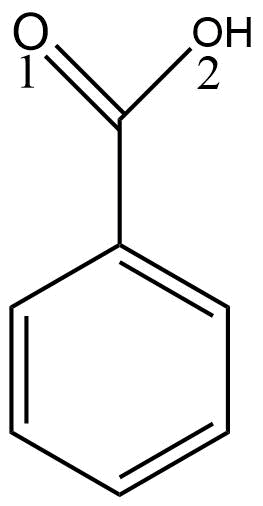
\includegraphics[width=0.1\linewidth]{pics/cocaine-chapter/bzacid_struct.png}
%\caption{Structure  of benzoic acid.}
%\label{fig:bzacid_struct}
%\end{figure} 




\subsection{Isobutyrate esters}
Methyl and ethyl isobutyrates (MeIsoBut and EtIsoBut) are of relevance for this study because of their similarity with the carboxylic acid ester moiety in cocaine and its analogues (see structure in \autoref{tab:structs2}).
%
The PTR-MS data for these two compounds was only acquired in normal conditions (i.e. no humid PTR-MS data is provided for MeIsoBut and EtIsoBut).

%\begin{figure}[htbp]
%\centering
%\includegraphics[width=0.4\linewidth]{pics/cocaine-chapter/isobuty_struct.png}
%\caption{Structure  of (left) methyl isobutyrate and  (right) ethyl isobutyrate.}
%\label{fig:isobuty_struct}
%\end{figure} 

\subsubsection{Methyl isobutyrate}

%(MeIso, C$_5$H$_{10}$O$_2$)
The PA and GB to yield the most stable structure of MeIsoButH$^+$ are .....\textbf{fill}...., and thus it can undergo proton transfer from....\textbf{fill}....
%
The product ion signal in counts per second from the reaction of MeIsoBut with (H$_2$O)$_n$H$_3$O$^+$ (n = 0, 1) are shown in \autoref{fig:EtIsoEN}. 
%
MeIsoButH$^+$ is the dominant ion through the whole range of \textit{E/N} values and fragmentation only occurs at high \textit{E/N}.
%

\begin{figure}[htbp]
\centering
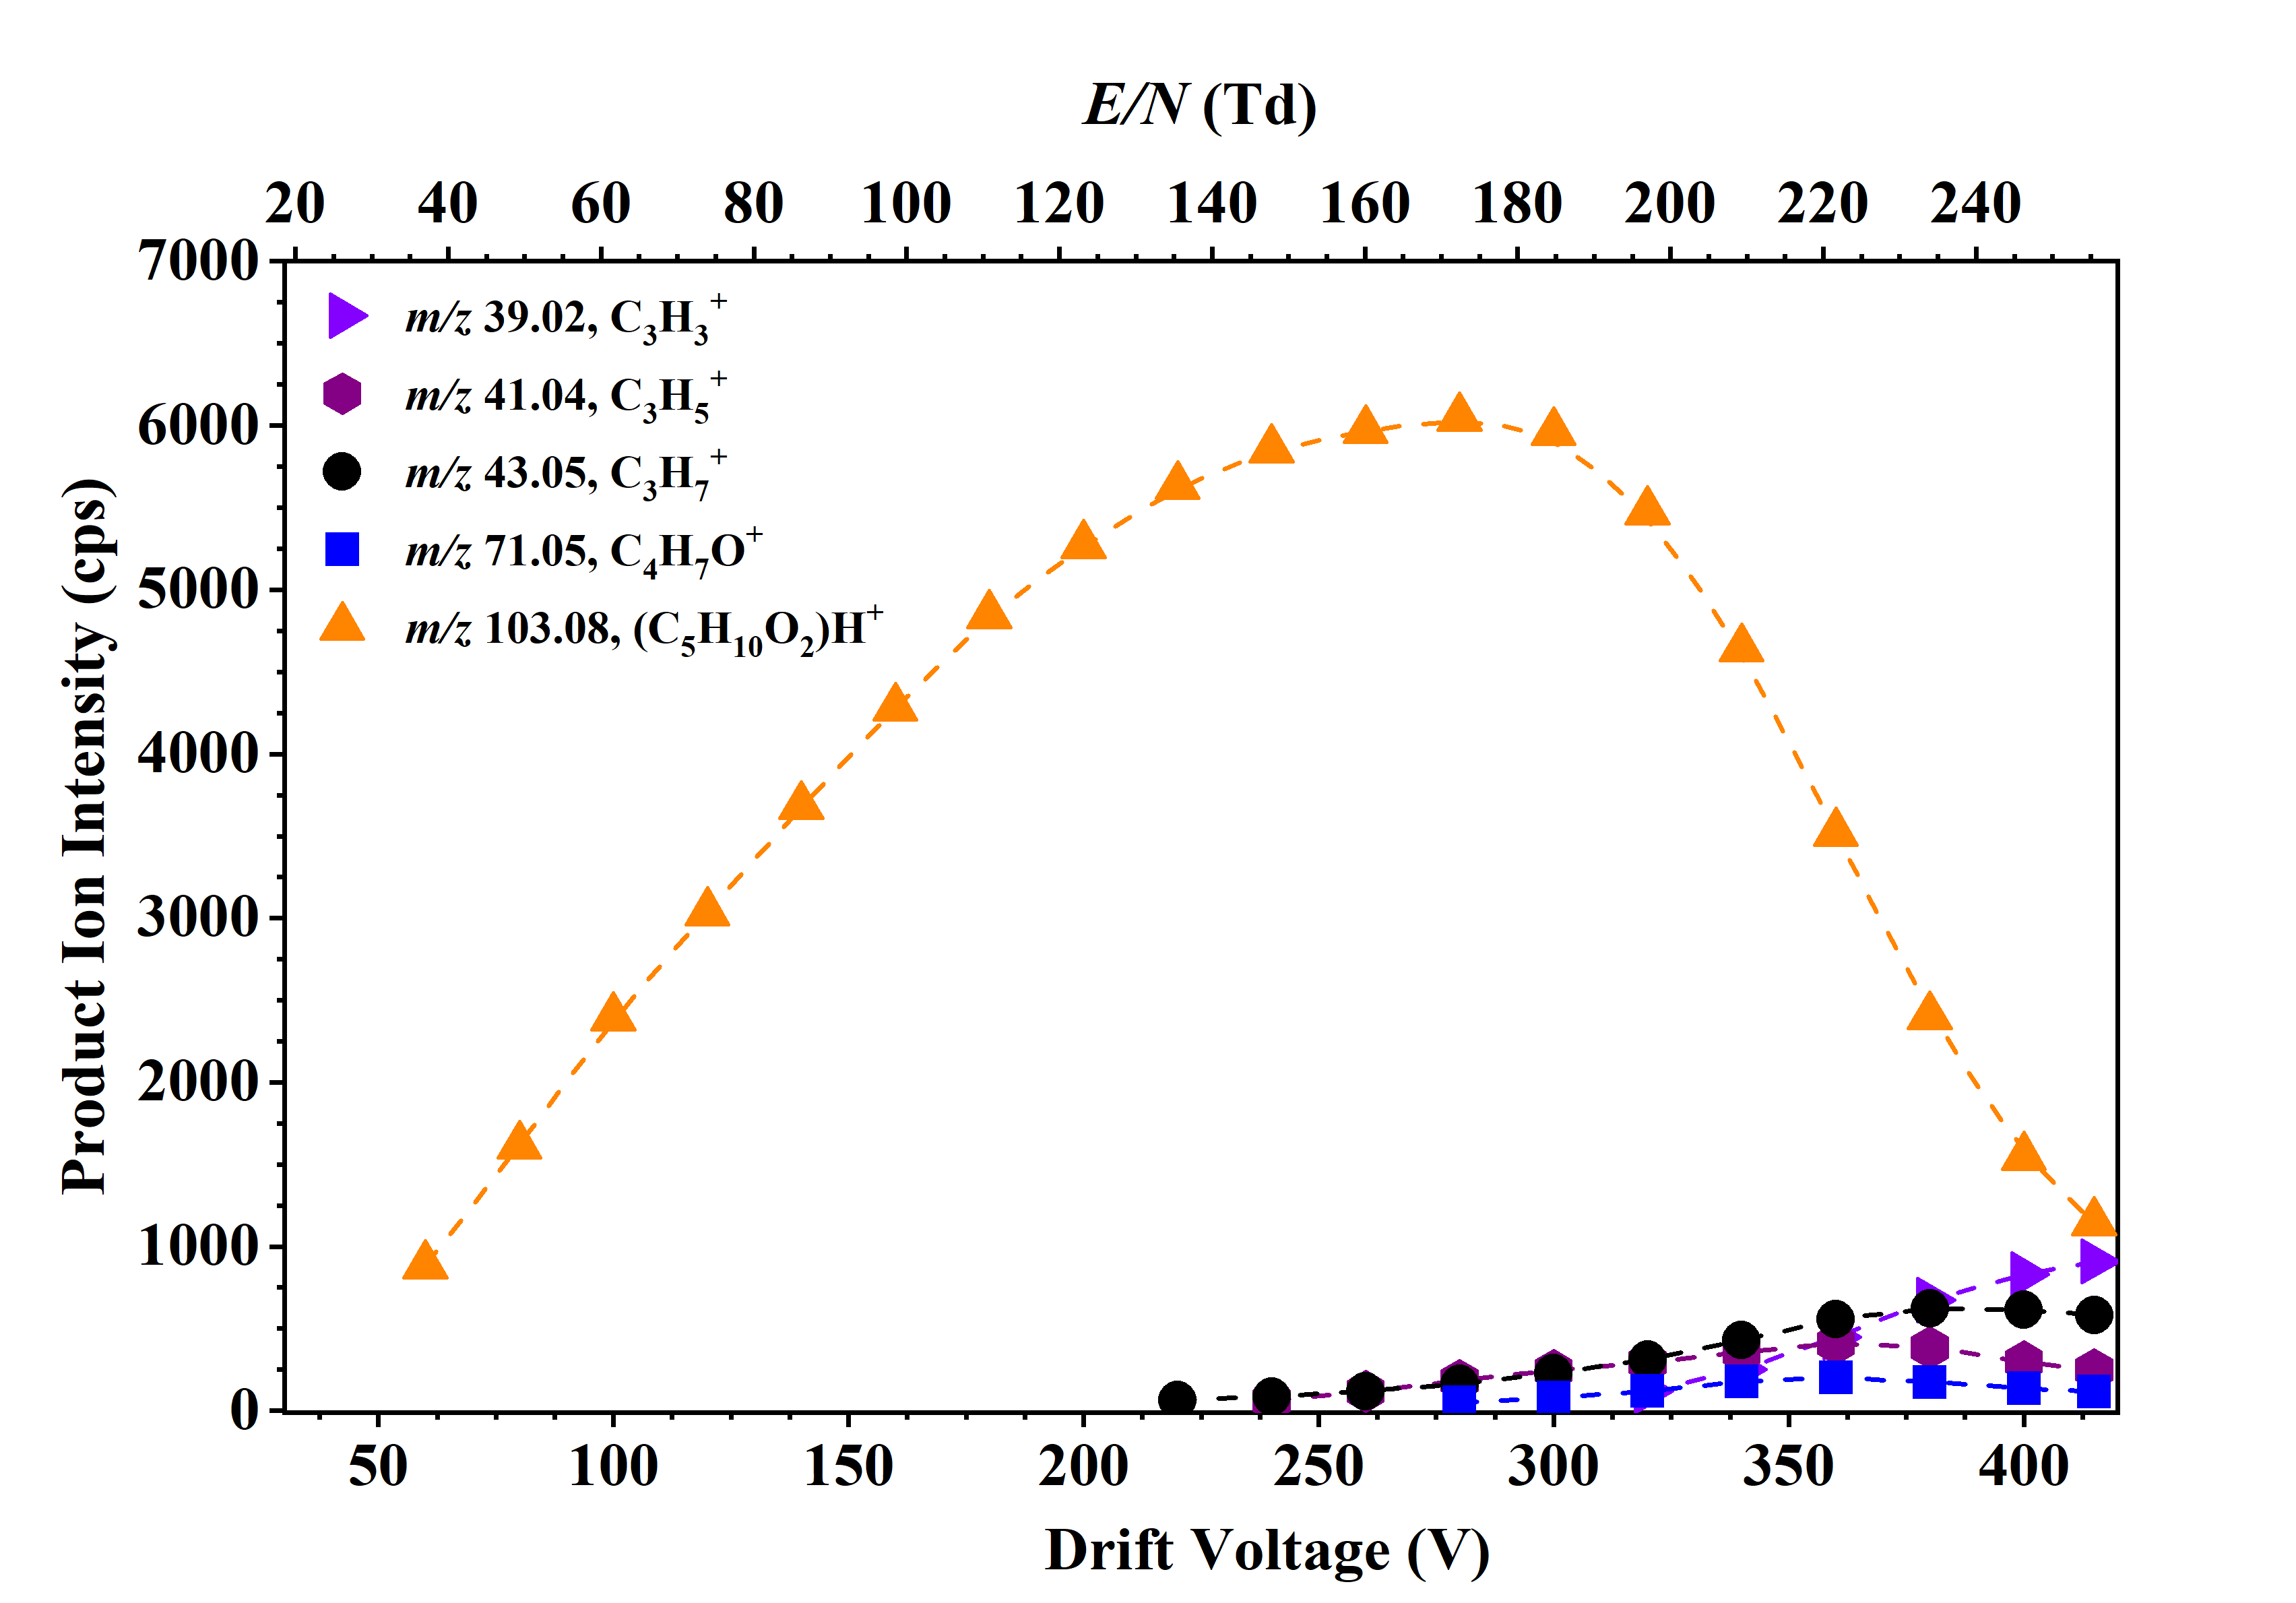
\includegraphics[width=0.8\linewidth]{pics/cocaine-chapter/MeIsobyturate-cps.png}
\caption{Product ion signal intensities in counts per second of the product ions resulting from reactions of the H$_3$O$^+$.(H$_2$O)$_n$ (n = 0, 1) with methyl isobutyrate as a function of the drift voltage and the reduced electric field.} 
\label{fig:MeIsoEN}
\end{figure}




As the loss of MeOH from MeBzH$^+$ is observed, the loss of MeOH from MeIsoButH$^+$ was expected as well because of the structural similarities between the benzoates and isobutyrates, 
but this is only observed at trace levels (\textit{m/z} 71) at high \textit{E/N}, which is surprising.
%
The $\Delta$G for the transition state 1H$^+$ to 2H$^+$ for MeIsoButH$^+$ is 34 kJ mol$^{-1}$, while for MeBzH$^+$ this is 14 kJ mol$^{-1}$.
%
This could  mislead to think that the loss of MeOH occurs through a transition state which MeBz can overcome with the energy from the field while MeIsoBut cannot.
%
However, this cannot be the reason because EtIsoBut has similar energetics to those of MeBz for the loss of MeOH but the loss of EtOH is only observed at high \textit{E/N} (see following section).
%
No proper answer has been found for this question as of yet.


%It was initially thought that the loss of MeOH in MeBz was due to direct protonation of O2 to give the structure MeBz2H$^+$ that steadily fragments to benzoyl$^+$ + MeOH because there is an endergonic transition state of +14 kJ mol$^{-1}$ from MeBz1H$^+$ to MeBz2H$^+$ that cannot operate.
%
%Loss of MeOH was also expected from protonated MeIsoBut because of the structural similarities between the benzoates and isobutyrates, but this is only observed at trace levels (\textit{m/z} 71) at high \textit{E/N}, which is surprising.
%
%These different finding can be however clarified by looking at the energetics of the transition state from the 1H$^+$ structure to the 2H$^+$ for these molecules: $\Delta$G$_{298}$(MeBz1H$^+$ to MeBz2H$^+$) = 14 kJ mol$^{-1}$ and $\Delta$G$_{298}$(MeIsoBut1H$^+$ to MeIsoBut2H$^+$) = 34 kJ mol$^{-1}$.
%
%It is then concluded that the loss of MeOH occurs through a transition state which MeBz can overcome with the energy from the field while MeIsoBut cannot.

%and it is then concluded that the transition state is the fragmentation that operates for the loss of MeOH in MeBz, not direct protonation of O2.




%%%%%%%%%%%%%%%%%%%%%%%%%%
%Significant fragmentation only occurs at high values of \textit{E/N} and is mainly concerned with the isobutyrate moiety. Only a trace of MeOH loss is observed. Whilst initially surprising, inspection of the associated TS shows it to be explicable – see below.

%It was suggested earlier that because of the endergonic TS for loss of MeOH following protonation of the carboxyl oxygen that the facile loss of MeOH from MeBz was due to direct protonation of the alkoxy oxygen. If this were so a similar facile loss of MeOH would be expected from MeIso. But but this is not observed. It is therefore concluded that the energy imparted from the field is sufficient to overcome the endergonic TS for MeBz but the higher TS for MeIsoBut. Need to return to MeBz and Etbz discussion.






\subsubsection{Ethyl isobutyrate}

%         (EtIsob, C$_6$H$_{12}$O$_2$)

Similarly to MeIsoBut, EtIsoBut can undergo proton transfer from (H$_2$O)$_n$H$_3$O$^+$ for n = 0 and 1, but not from higher order clusters.
%
The energetics for the structures arising from the reaction of ethyl isobutyrate and (H$_2$O)$_n$H$_3$O$^+$ (n = 0, 1) are provided in \autoref{tb:EtIso2} and the product ion signal in cps as a function of the drift voltage and the reduced electric field for the same reaction are given in \autoref{fig:EtIsoEN}.



\begin{figure}[htbp]
\centering
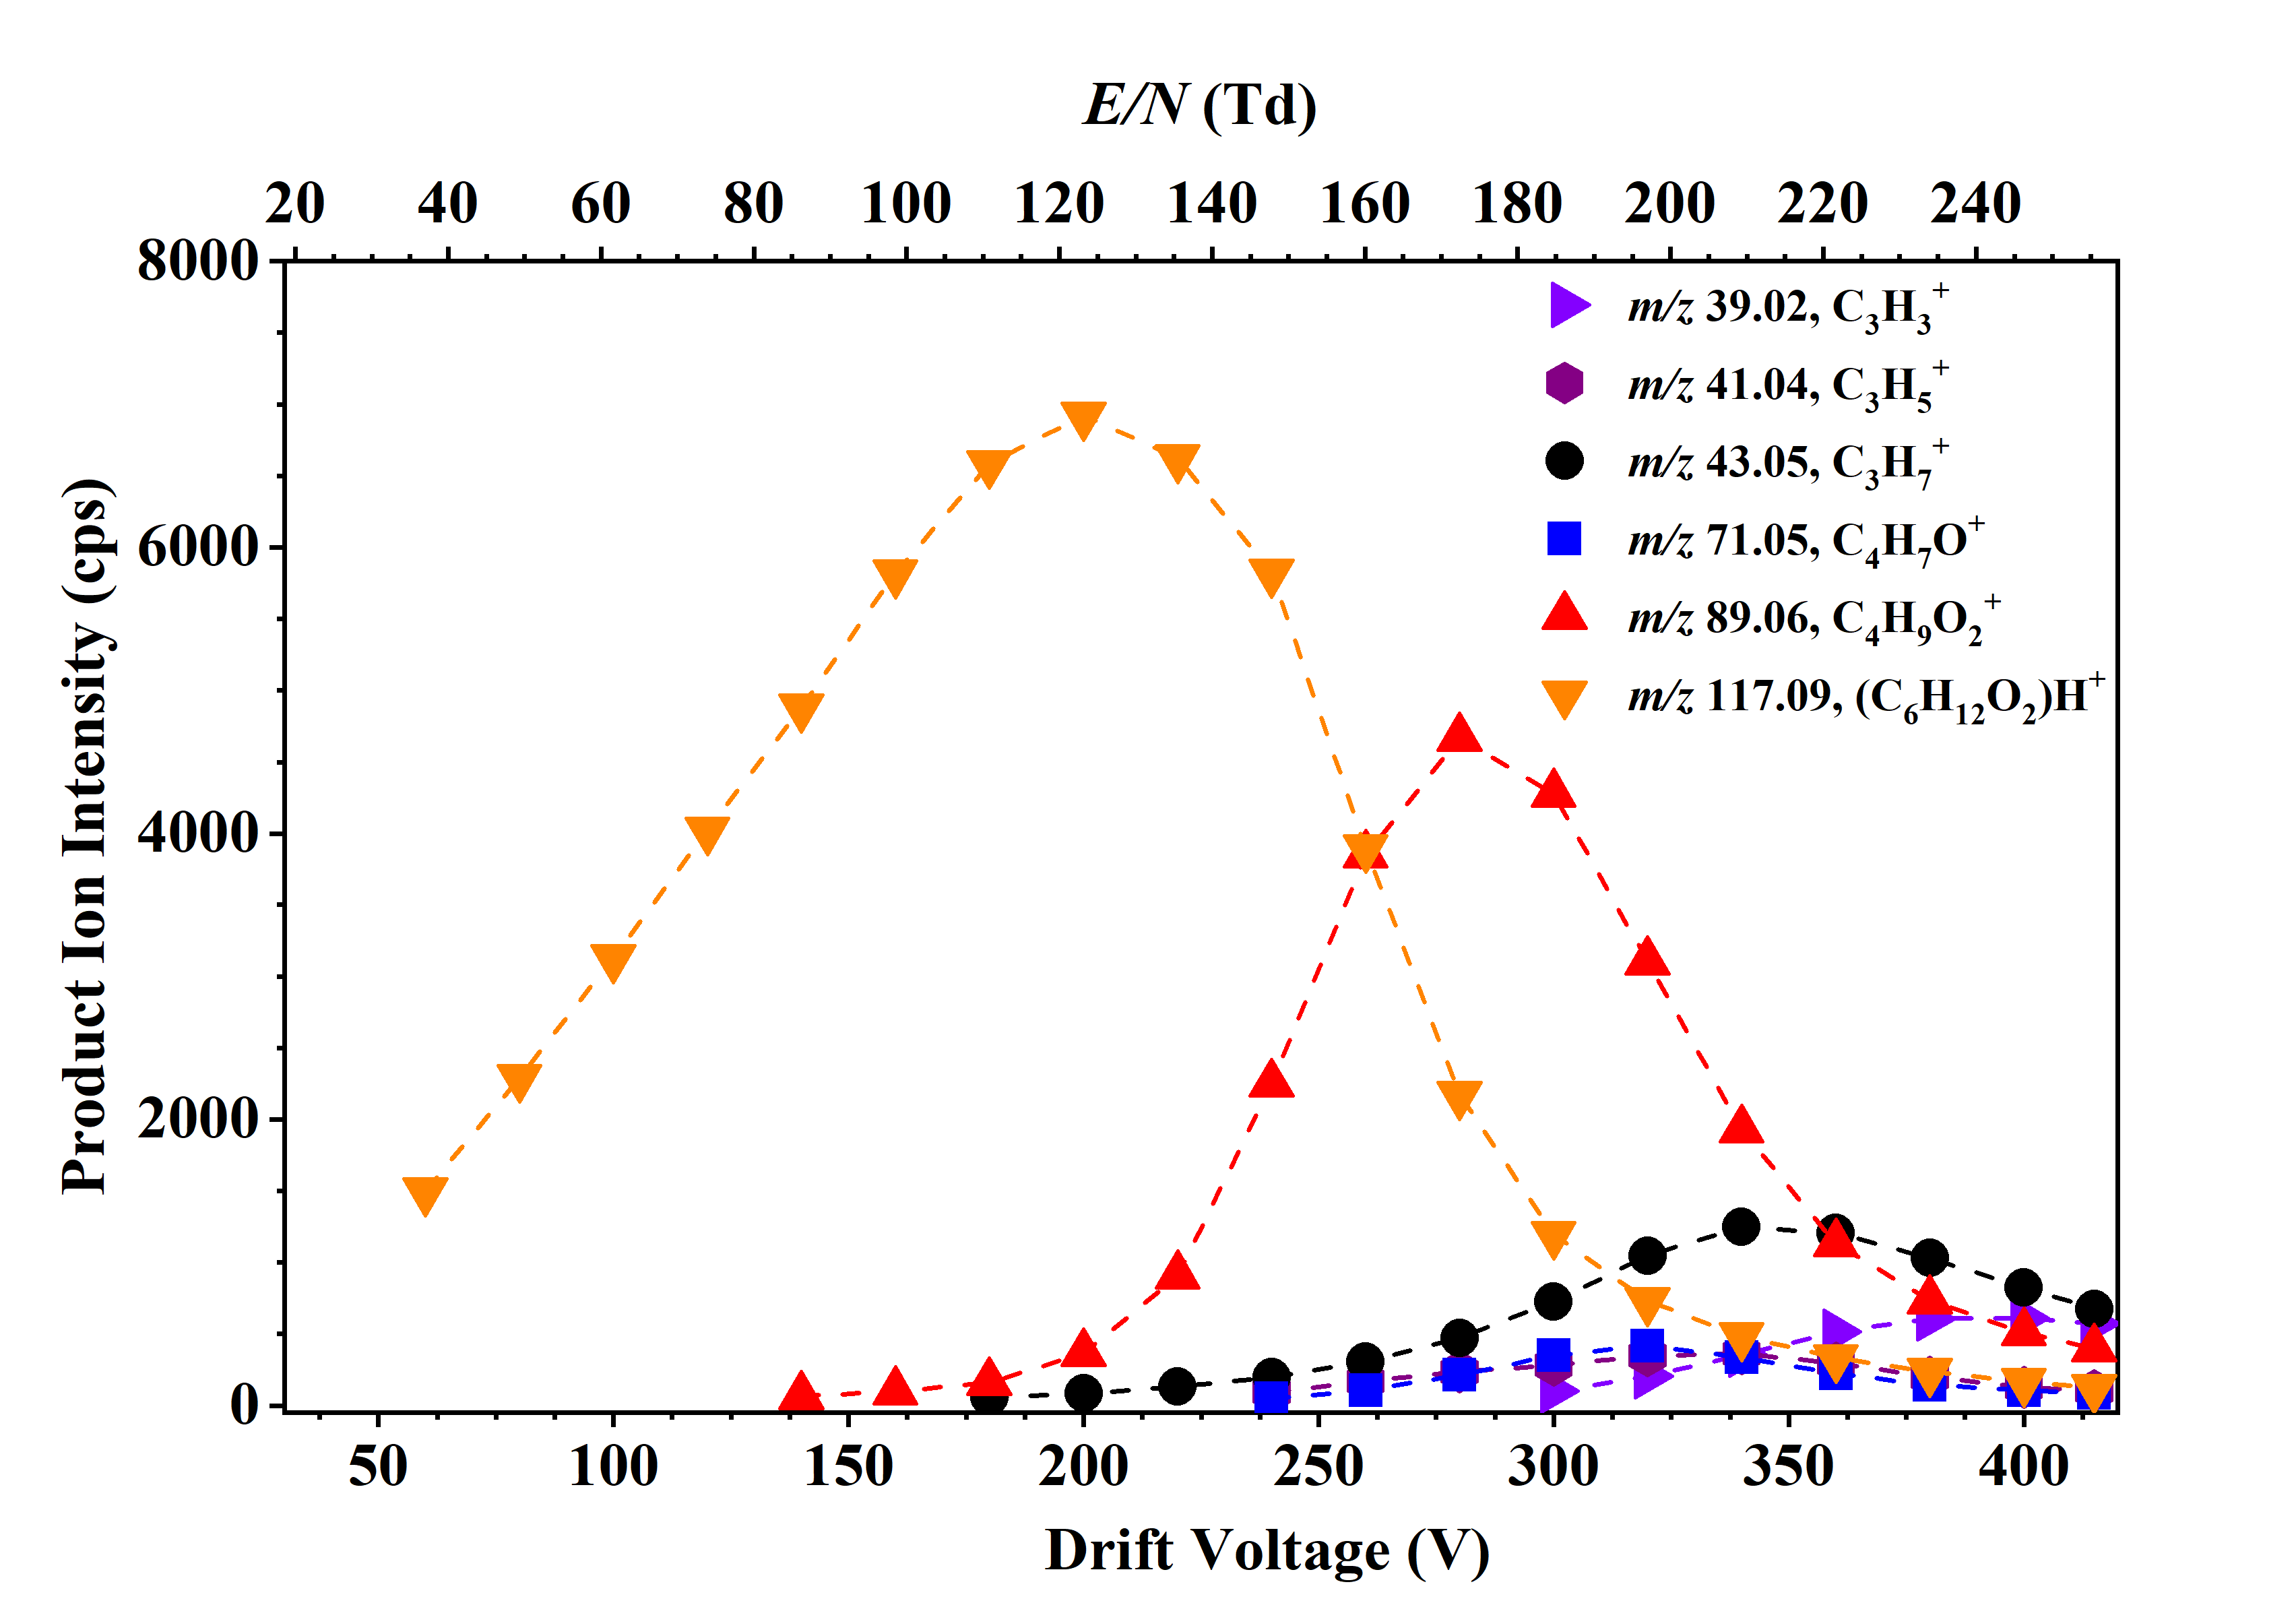
\includegraphics[width=0.8\linewidth]{pics/cocaine-chapter/EtIsobyturate-cps.png}
\caption{Product ion signal intensities in counts per second of the product ions resulting from reactions of the H$_3$O$^+$.(H$_2$O)$_n$ (n = 0, 1) with ethyl isobutyrate as a function of the drift voltage and the reduced electric field.} 
\label{fig:EtIsoEN}
\end{figure}

\begin{table}[htbp]
\centering
\caption{Energetics relative to ethyl isobutyrate and H$_3$O$^+$ and, in brackets, to ethyl isobutyrate and (H$_2$O)H$_3$O$^+$.}
\label{tb:EtIso2}
\begin{tabular}{lccc}
\toprule
\textbf{Reaction or transition state}	&\textbf{\textit{m/z} } &\textbf{$\Delta$H$_{298}$} &\textbf{$\Delta$G$_{298}$}\\
& &	\textbf{(kJ/mol)} &\textbf{(kJ/mol)} \\  \toprule
EtIsoBut1H$^+$ & 117 & -145 (+13) & -146 (-22) \\ \midrule
EtIsoBut2H$^+$ & 117 & -81 (+77) & -86 (+38) \\ \midrule
IsoButyryl$^+$ + EtOH & 71 & -9 (+149) & -59 (+65) \\ \midrule
TS 1H$^+$ to 2H$^+$ &  & +18 (+176) & +17 (+141) \\ \midrule
IsoButyric acidH$^+$ + C$_2$H$_4$ & 89 & -38 (+120) & -85 (+39) \\ \midrule
TS1 loss of ethene  &  & -28 (+130) & -34 (+90) \\ \midrule
TS2 loss of ethene  &  & -6 (+152) & -11 (+113) \\
\bottomrule
\end{tabular}
\end{table}




The main fragment ion is the loss of ethene at \textit{m/z} 89 to yield isobutyric acidH$^+$.
%
This fragmentation pathway resembles the one for EtBz to yield BzAcidH$^+$.
%
Furthermore, the energetics for the transition states TS1 and TS2, which are similar to those explained in the EtBz section, are comparable and hence the loss of ethene must be the result of collision-induced dissociation for EtIsoBut as it was concluded for EtBz.
%


The interesting finding in \autoref{tb:EtIso2} is that the energetics of the transition state 1H$^+$ to 2H$^+$ are comparable to those of MeBz, so loss of EtOH from EtIsoBut was expected but it was not found in the PTR-MS data.
%
Therefore, the loss of MeOH or EtOH does not occur through the transition state, but via direct protonation of the alkoxy oxygen O2, as stated in the benzoate esters section.










%%%%%%%%%%%%%%%%%%%%%%%%%%%%%%%%%%%%%%%%%%%%%%%
%The dominant fragmentation is loss of ethene; the remaining fragmentations are similar to those observed with MeIsoBut i.e. only occur at high values of \textit{E/N} with most being concerned with the isobutyrate moiety and a trace of loss of EtOH.

% It can be seen that protonation by H$_3$O$^+$ should lead to ethene loss. That it does not occur below 100Td suggests that observed MH$^+$ is formed from (H$_2$O)H$_3$O$^+$. Above 100Td production of ethene may occur by direction protonation by H$_3$O$^+$ or field activation of MH$^+$ or probably both.


\subsection{Cocaethylene}
Cocaethylene is a product of the transesterification between cocaine and ethanol.
%



The product ion signal intensities of the product ions resulting from the reaction of cocaethylene with (H$_2$O)$_n$H$_3$O$^+$ as a function of the drift voltage and the reduced electric field are given in \autoref{fig:cocaetEN}.
%
These indicate that the fragmentation pathways and energetics are very similar to those of cocaine.
%
The dominant ion for the whole \textit{E/N} range in both normal and humid conditions is the protonated parent molecule.
%
Some minor product ions are those resulting from 
the loss of benzoic acid at \textit{m/z} 196 and 
the loss of EtOH at \textit{m/z} 272.
%
Traces of C$_5$H$_8$N$^+$ at \textit{m/z} 82 are found in the normal conditions measurement at high \textit{E/N} (i.e. >200 Td).

\begin{figure}[htbp]
\centering
\sidesubfloat[]{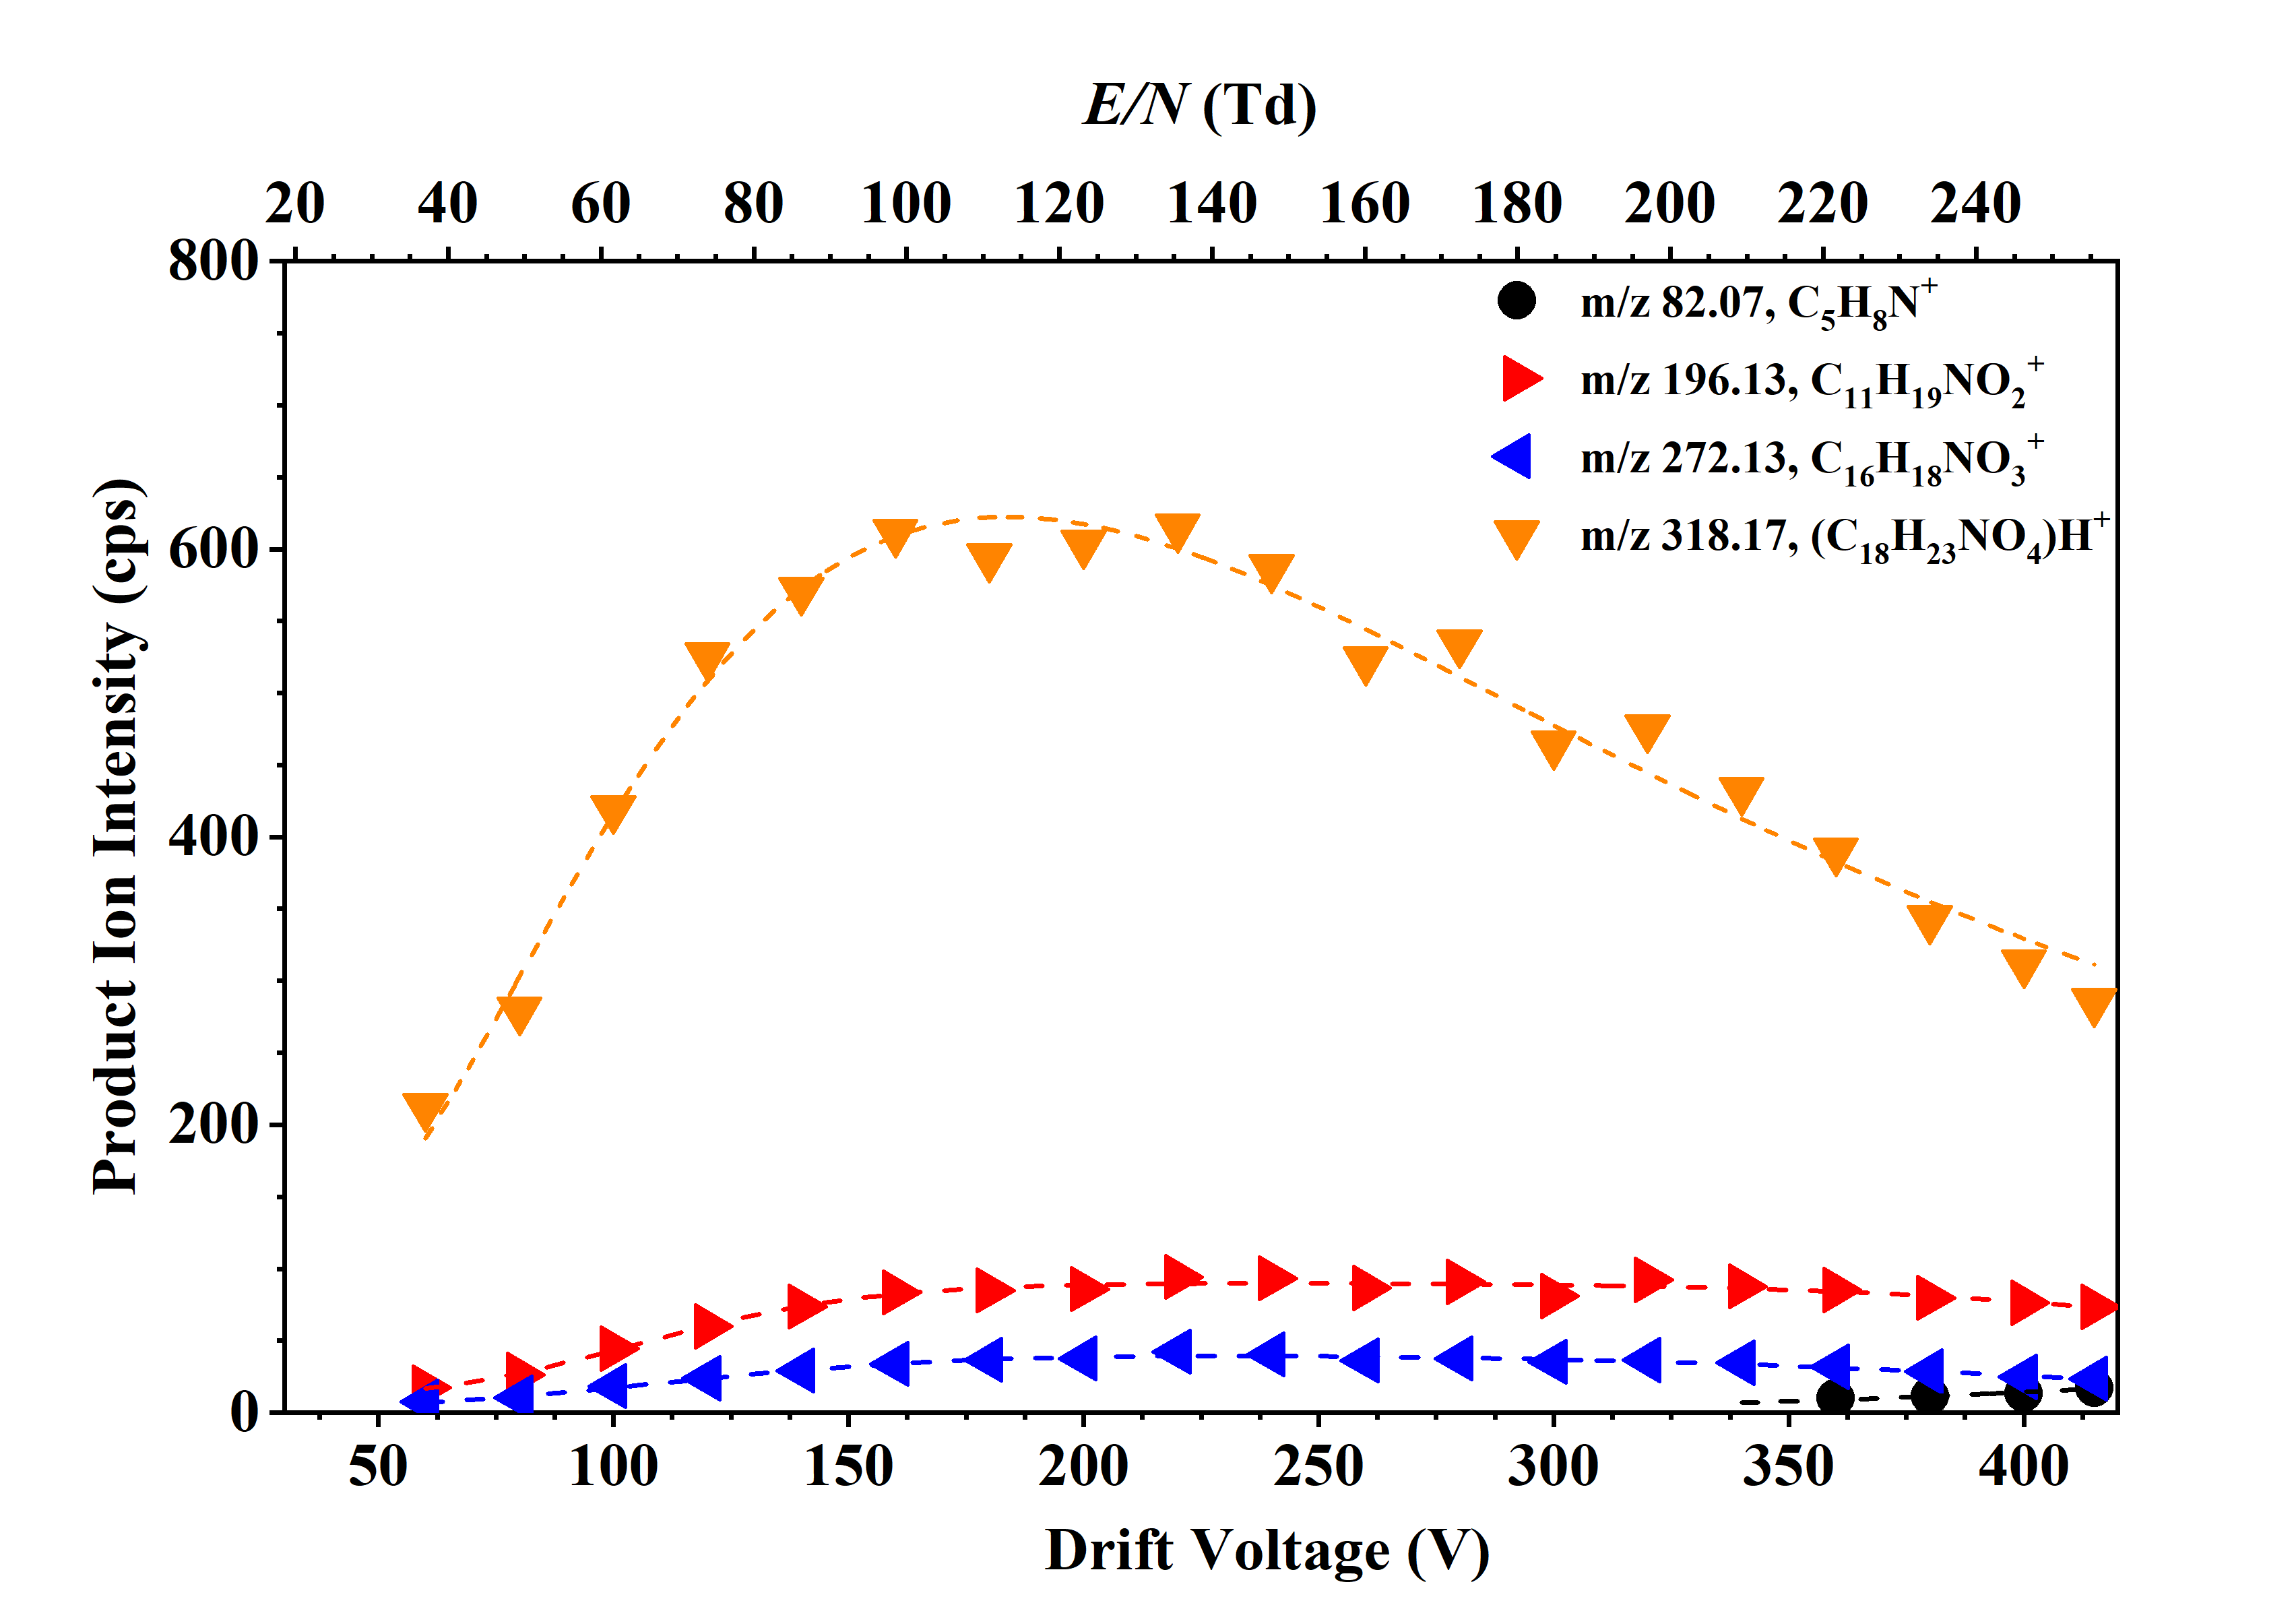
\includegraphics[width=0.8\linewidth]{pics/cocaine-chapter/cocaethylene-cps.png}}\\
\sidesubfloat[]{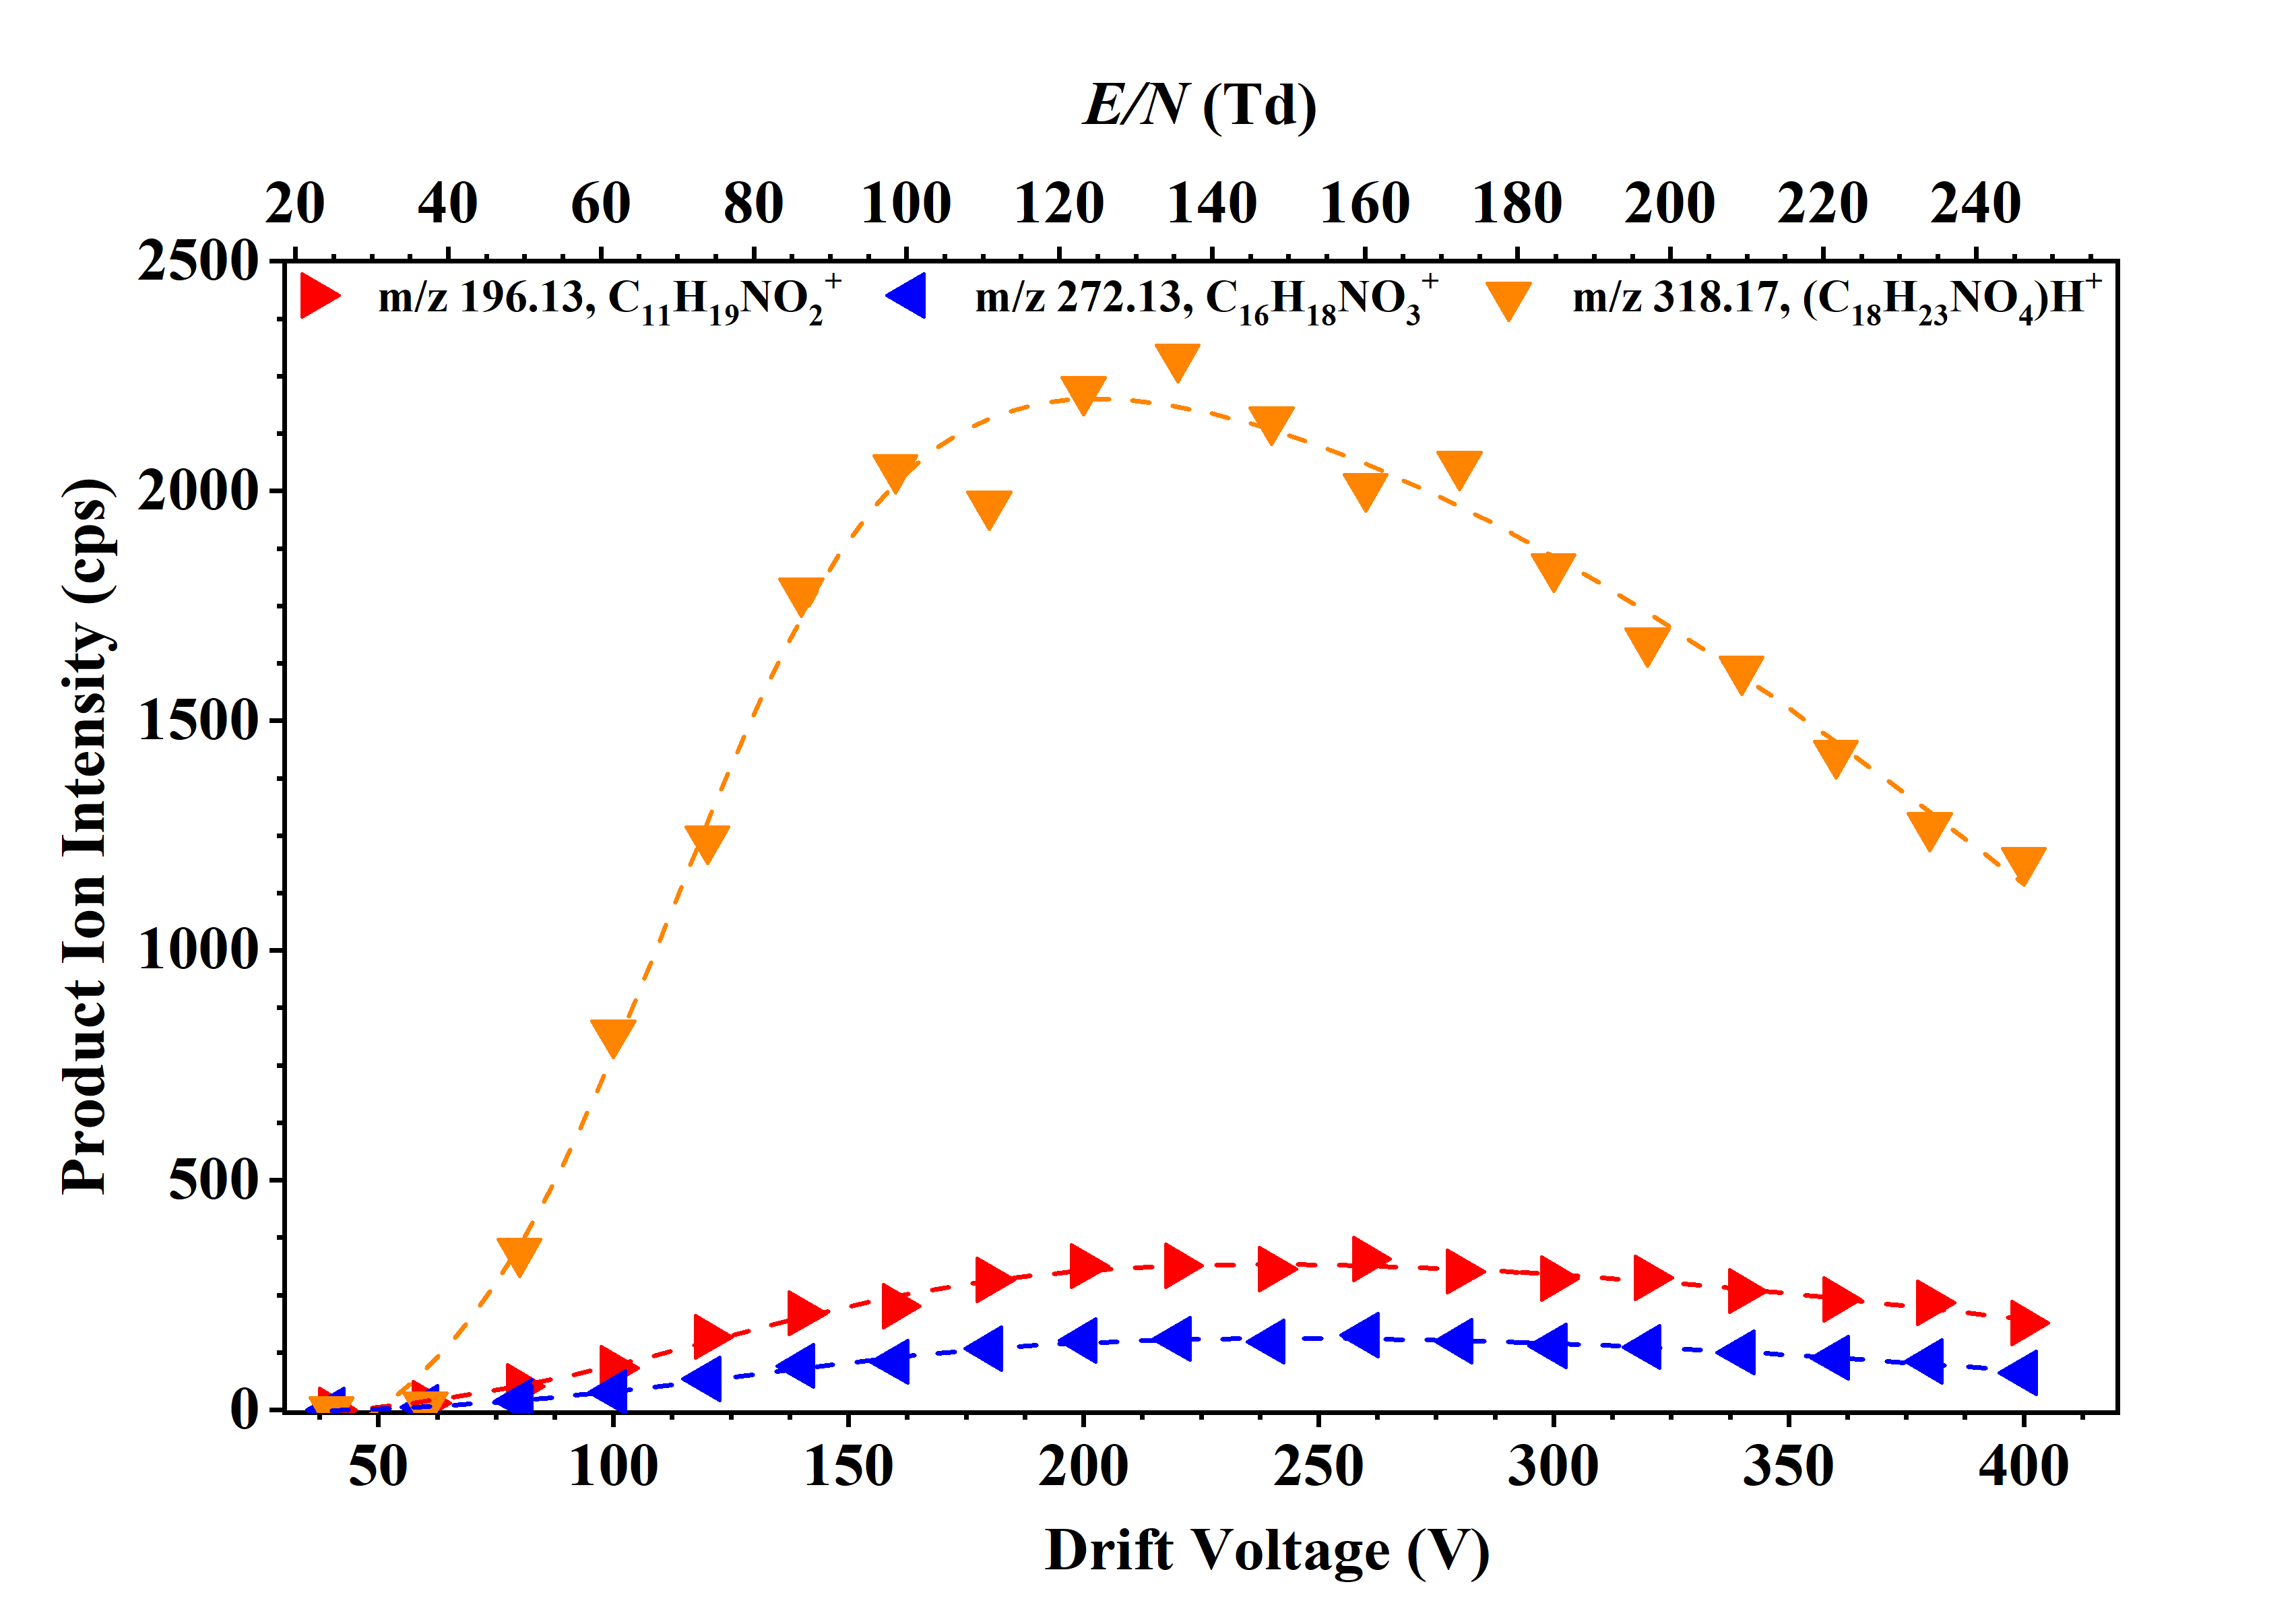
\includegraphics[width=0.8\linewidth]{pics/cocaine-chapter/humid/cocaethylene-cps.png}}
\caption{Product ion signal intensities in counts per second of the product ions resulting from reactions of the H$_3$O$^+$.(H$_2$O)$_n$ (n = 0, 1, 2) with cocaethylene as a function of the drift voltage and the reduced electric field in (a) normal and (b) humid conditions.}
\label{fig:cocaetEN}
\end{figure}










%\begin{figure}[htbp]
%\centering
%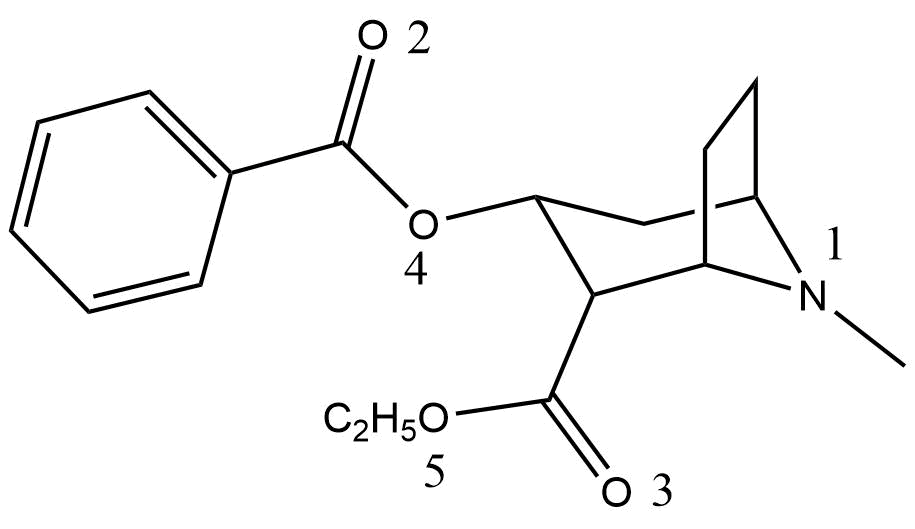
\includegraphics[width=0.4\linewidth]{pics/cocaine-chapter/cocaet_struct.png}
%\caption{Structure  of cocaethylene, including the numbering of the main protonation sites.}
%\label{fig:cocaet_struct}
%\end{figure}

 
 




\subsection{Ethyl ecgonine}


\begin{figure}[htbp]
\centering
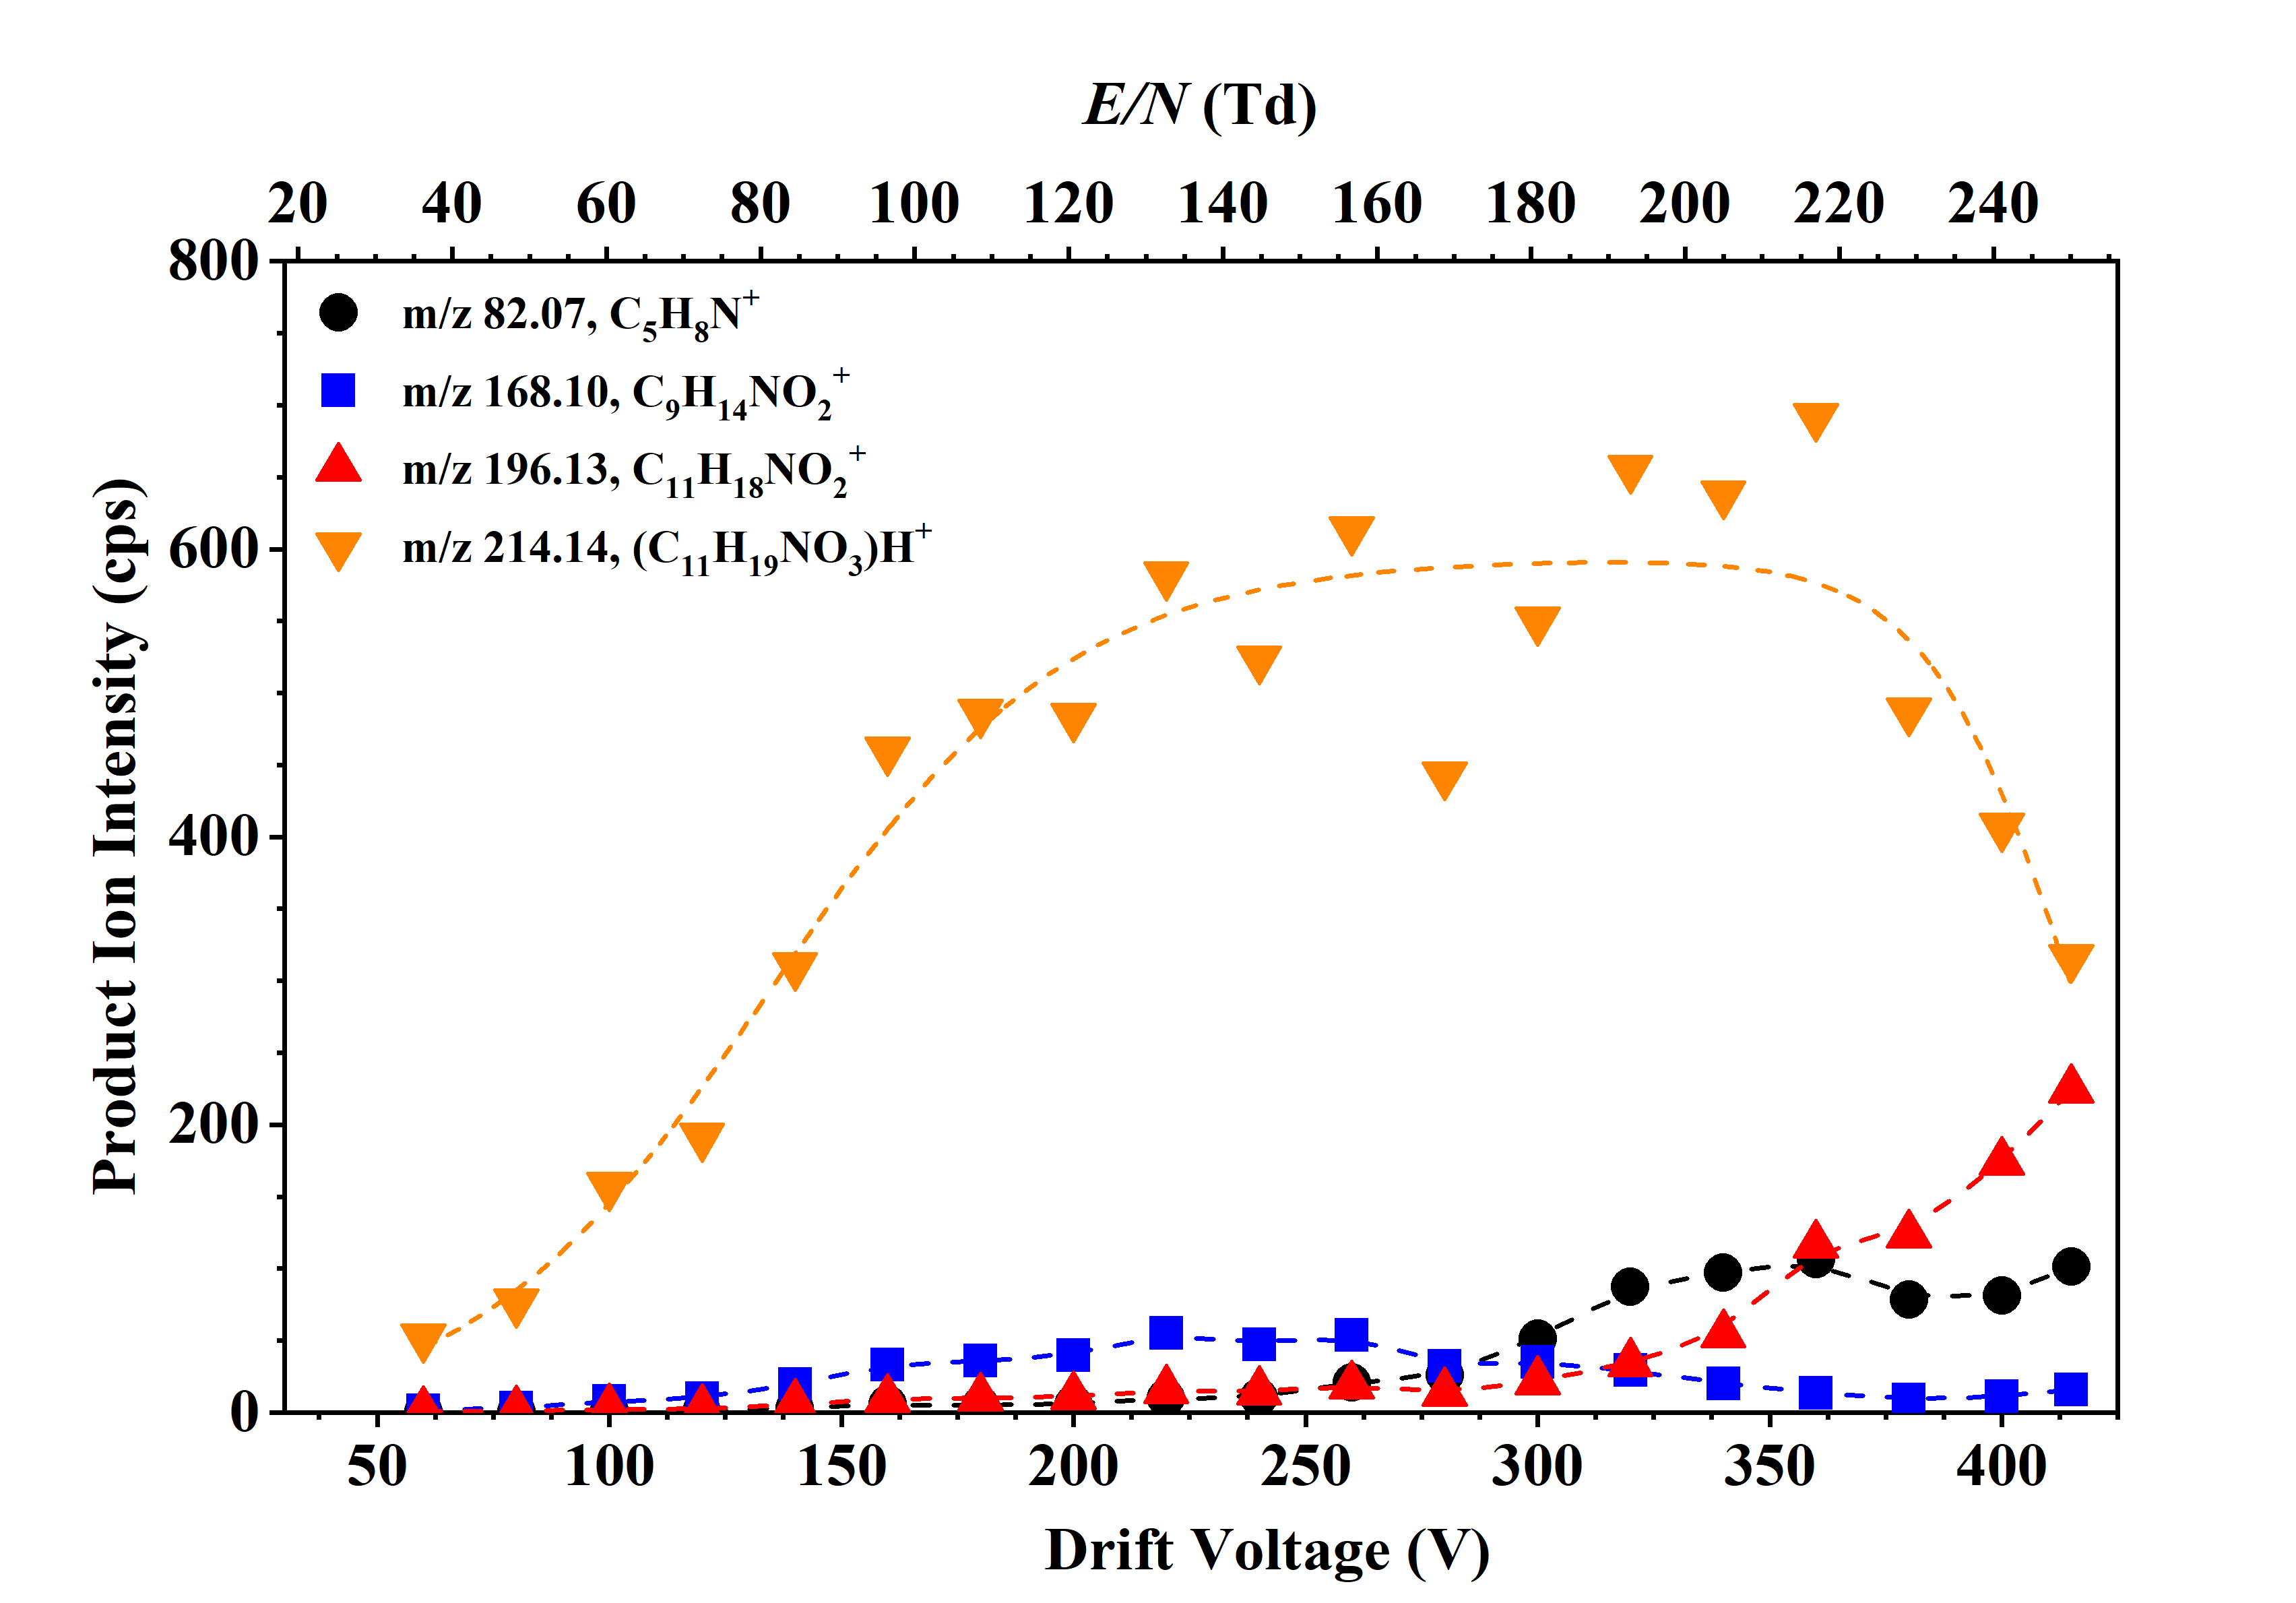
\includegraphics[width=0.8\linewidth]{pics/cocaine-chapter/EtEcg-cps.png}
\caption{Product ion signal intensities in counts per second of the product ions resulting from reactions of the H$_3$O$^+$.(H$_2$O)$_n$ (n = 0, 1, 2) with ethyl ecgonine as a function of the drift voltage and the reduced electric field.} 
\label{fig:etecgEN}
\end{figure}


\subsection{Norcocaine}
Norcocaine (


The ion at \textit{m/z} 68 is similar to that found in cocaine, cocaethylene, methyl ecgonine and ethyl ecgonine at \textit{m/z} 82.









\begin{figure}[htbp]
\centering
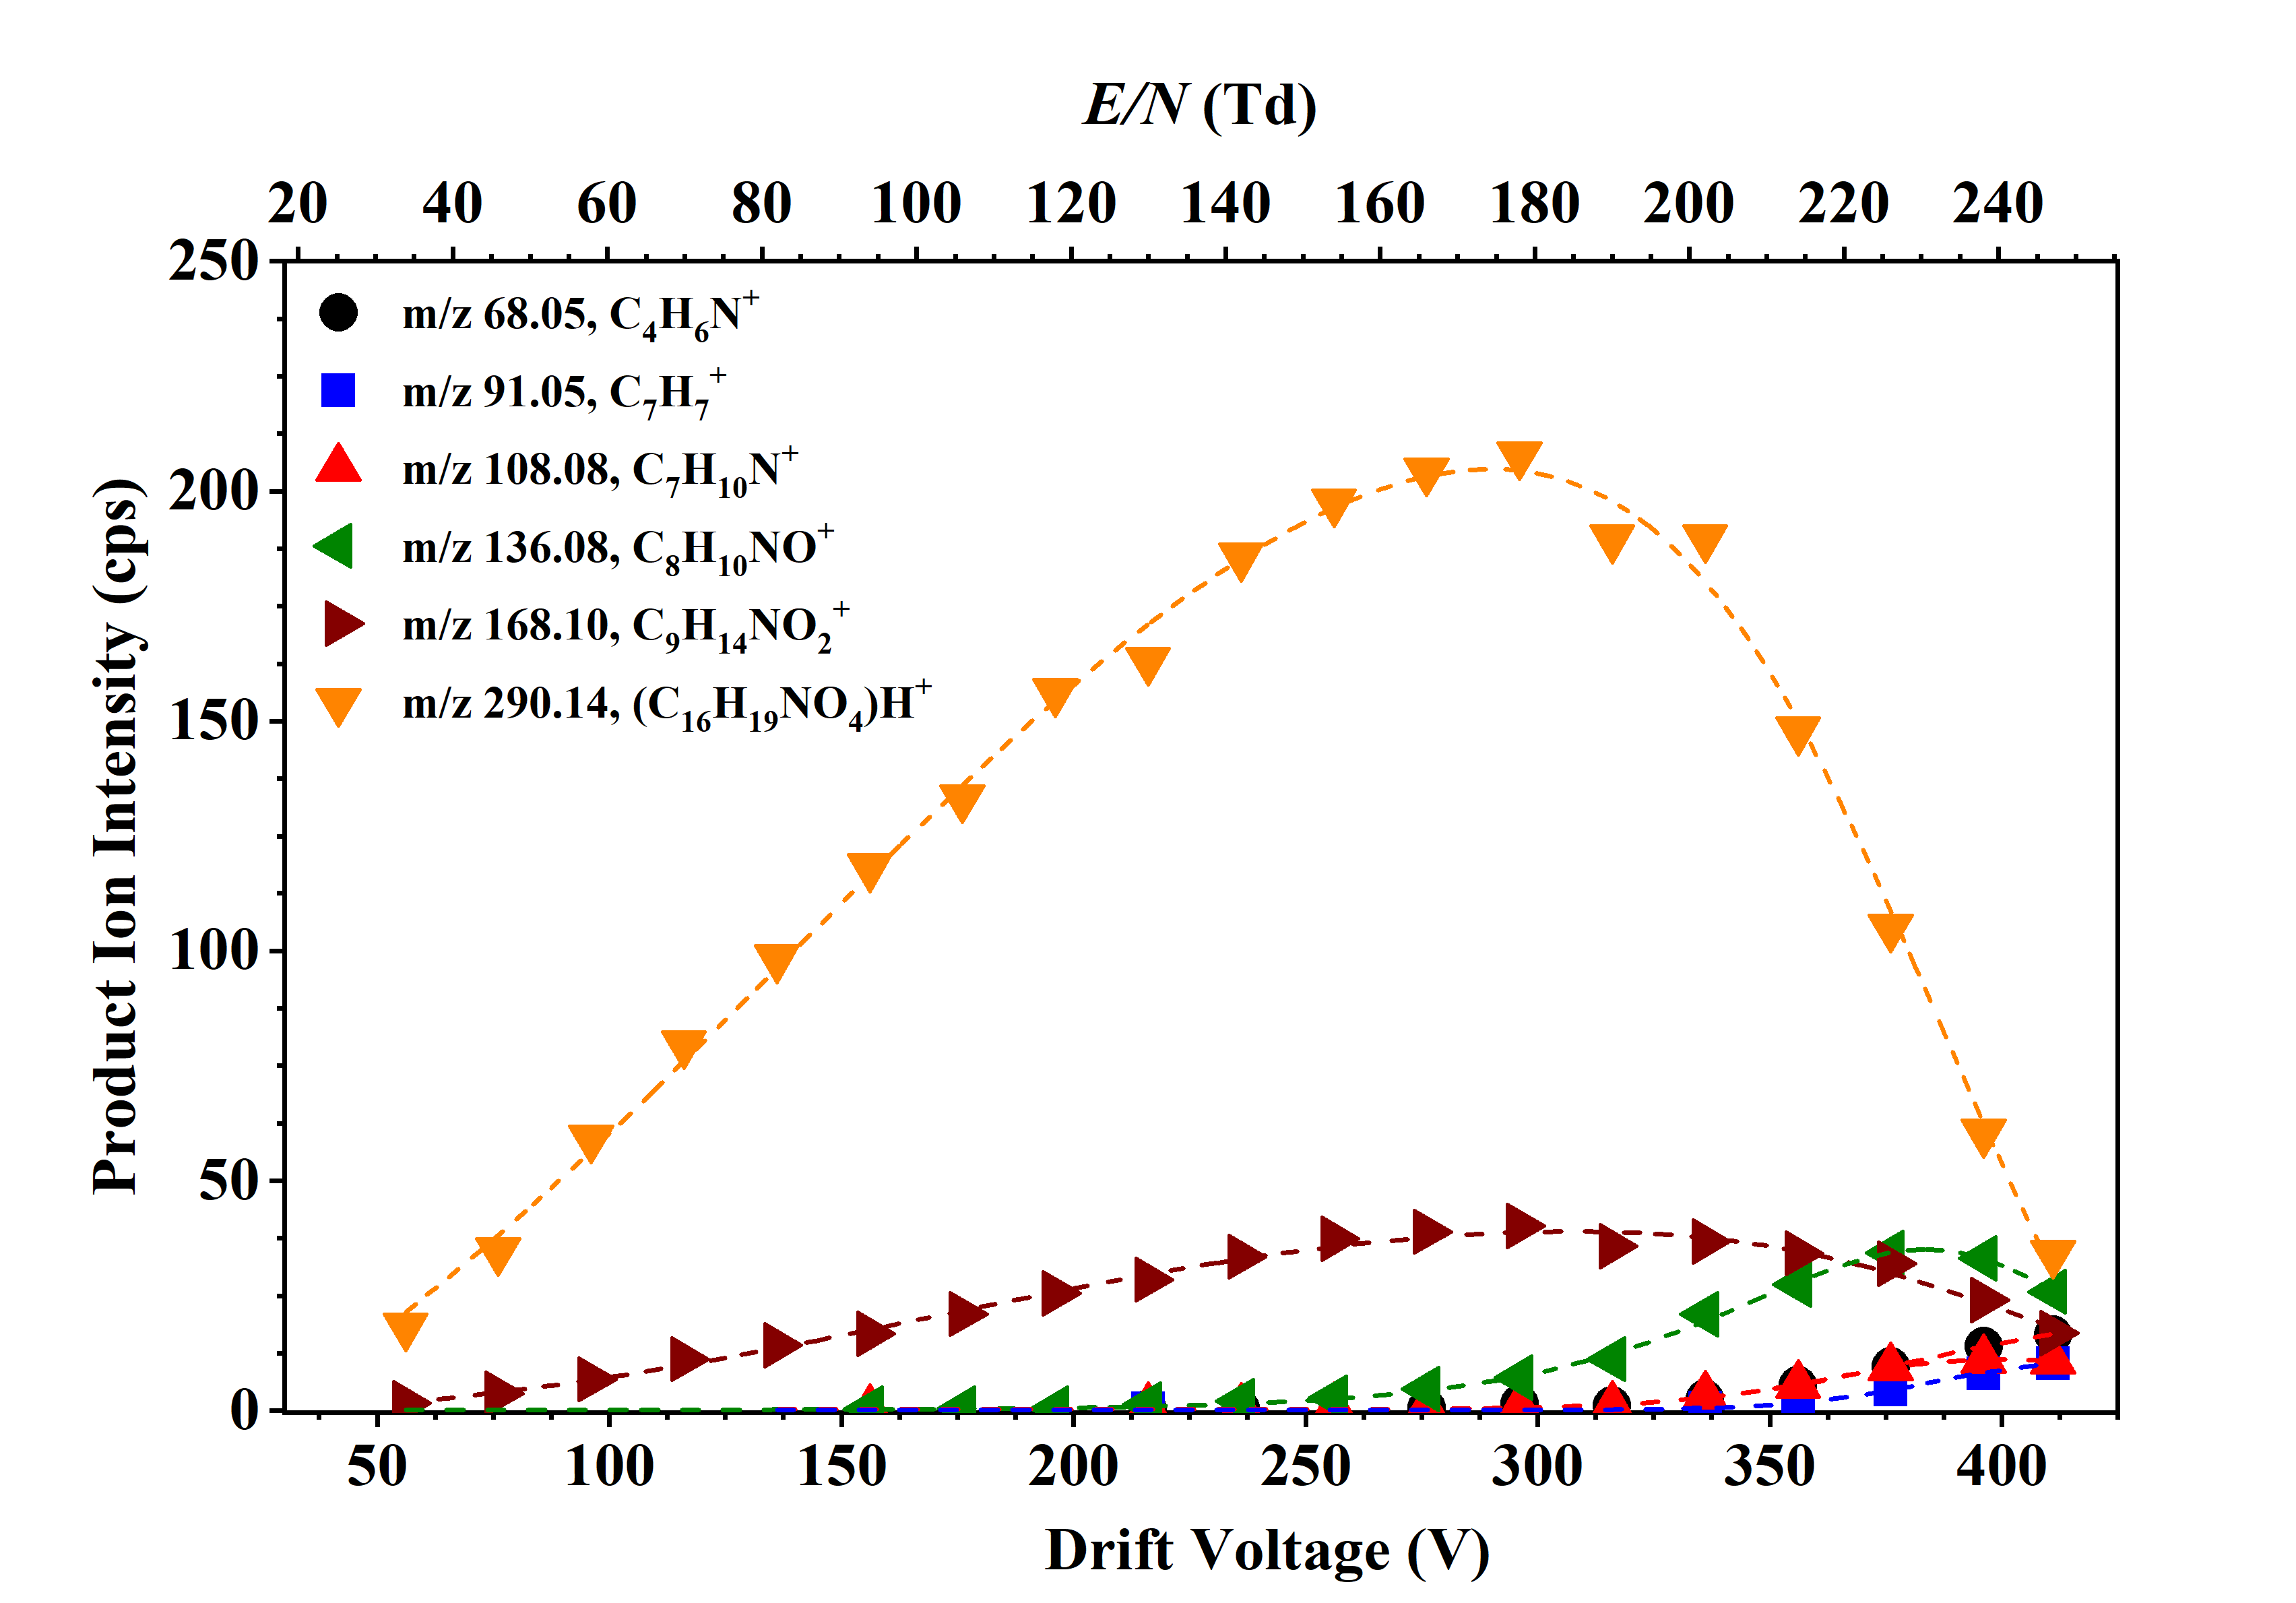
\includegraphics[width=0.8\linewidth]{pics/cocaine-chapter/norcocaine-cps.png}
\caption{Product ion signal intensities in counts per second of the product ions resulting from reactions of the H$_3$O$^+$.(H$_2$O)$_n$ (n = 0, 1, 2) with norcocaine as a function of the drift voltage and the reduced electric field.} 
\label{fig:norcocaEN}
\end{figure}


\subsection{Methyl ecgonidine}
Methyl ecgonidine (C$_{10}$H$_{15}$NO$_2$, also known as anhydroecgonine methyl ester) is the main pyrolysis product of cocaine. It is formed when the drug is decomposed at high temperatures and it has been found to be excreted by crack smokers \cite{anhydroecgoninemethylester}.





\begin{figure}[htbp]
\centering
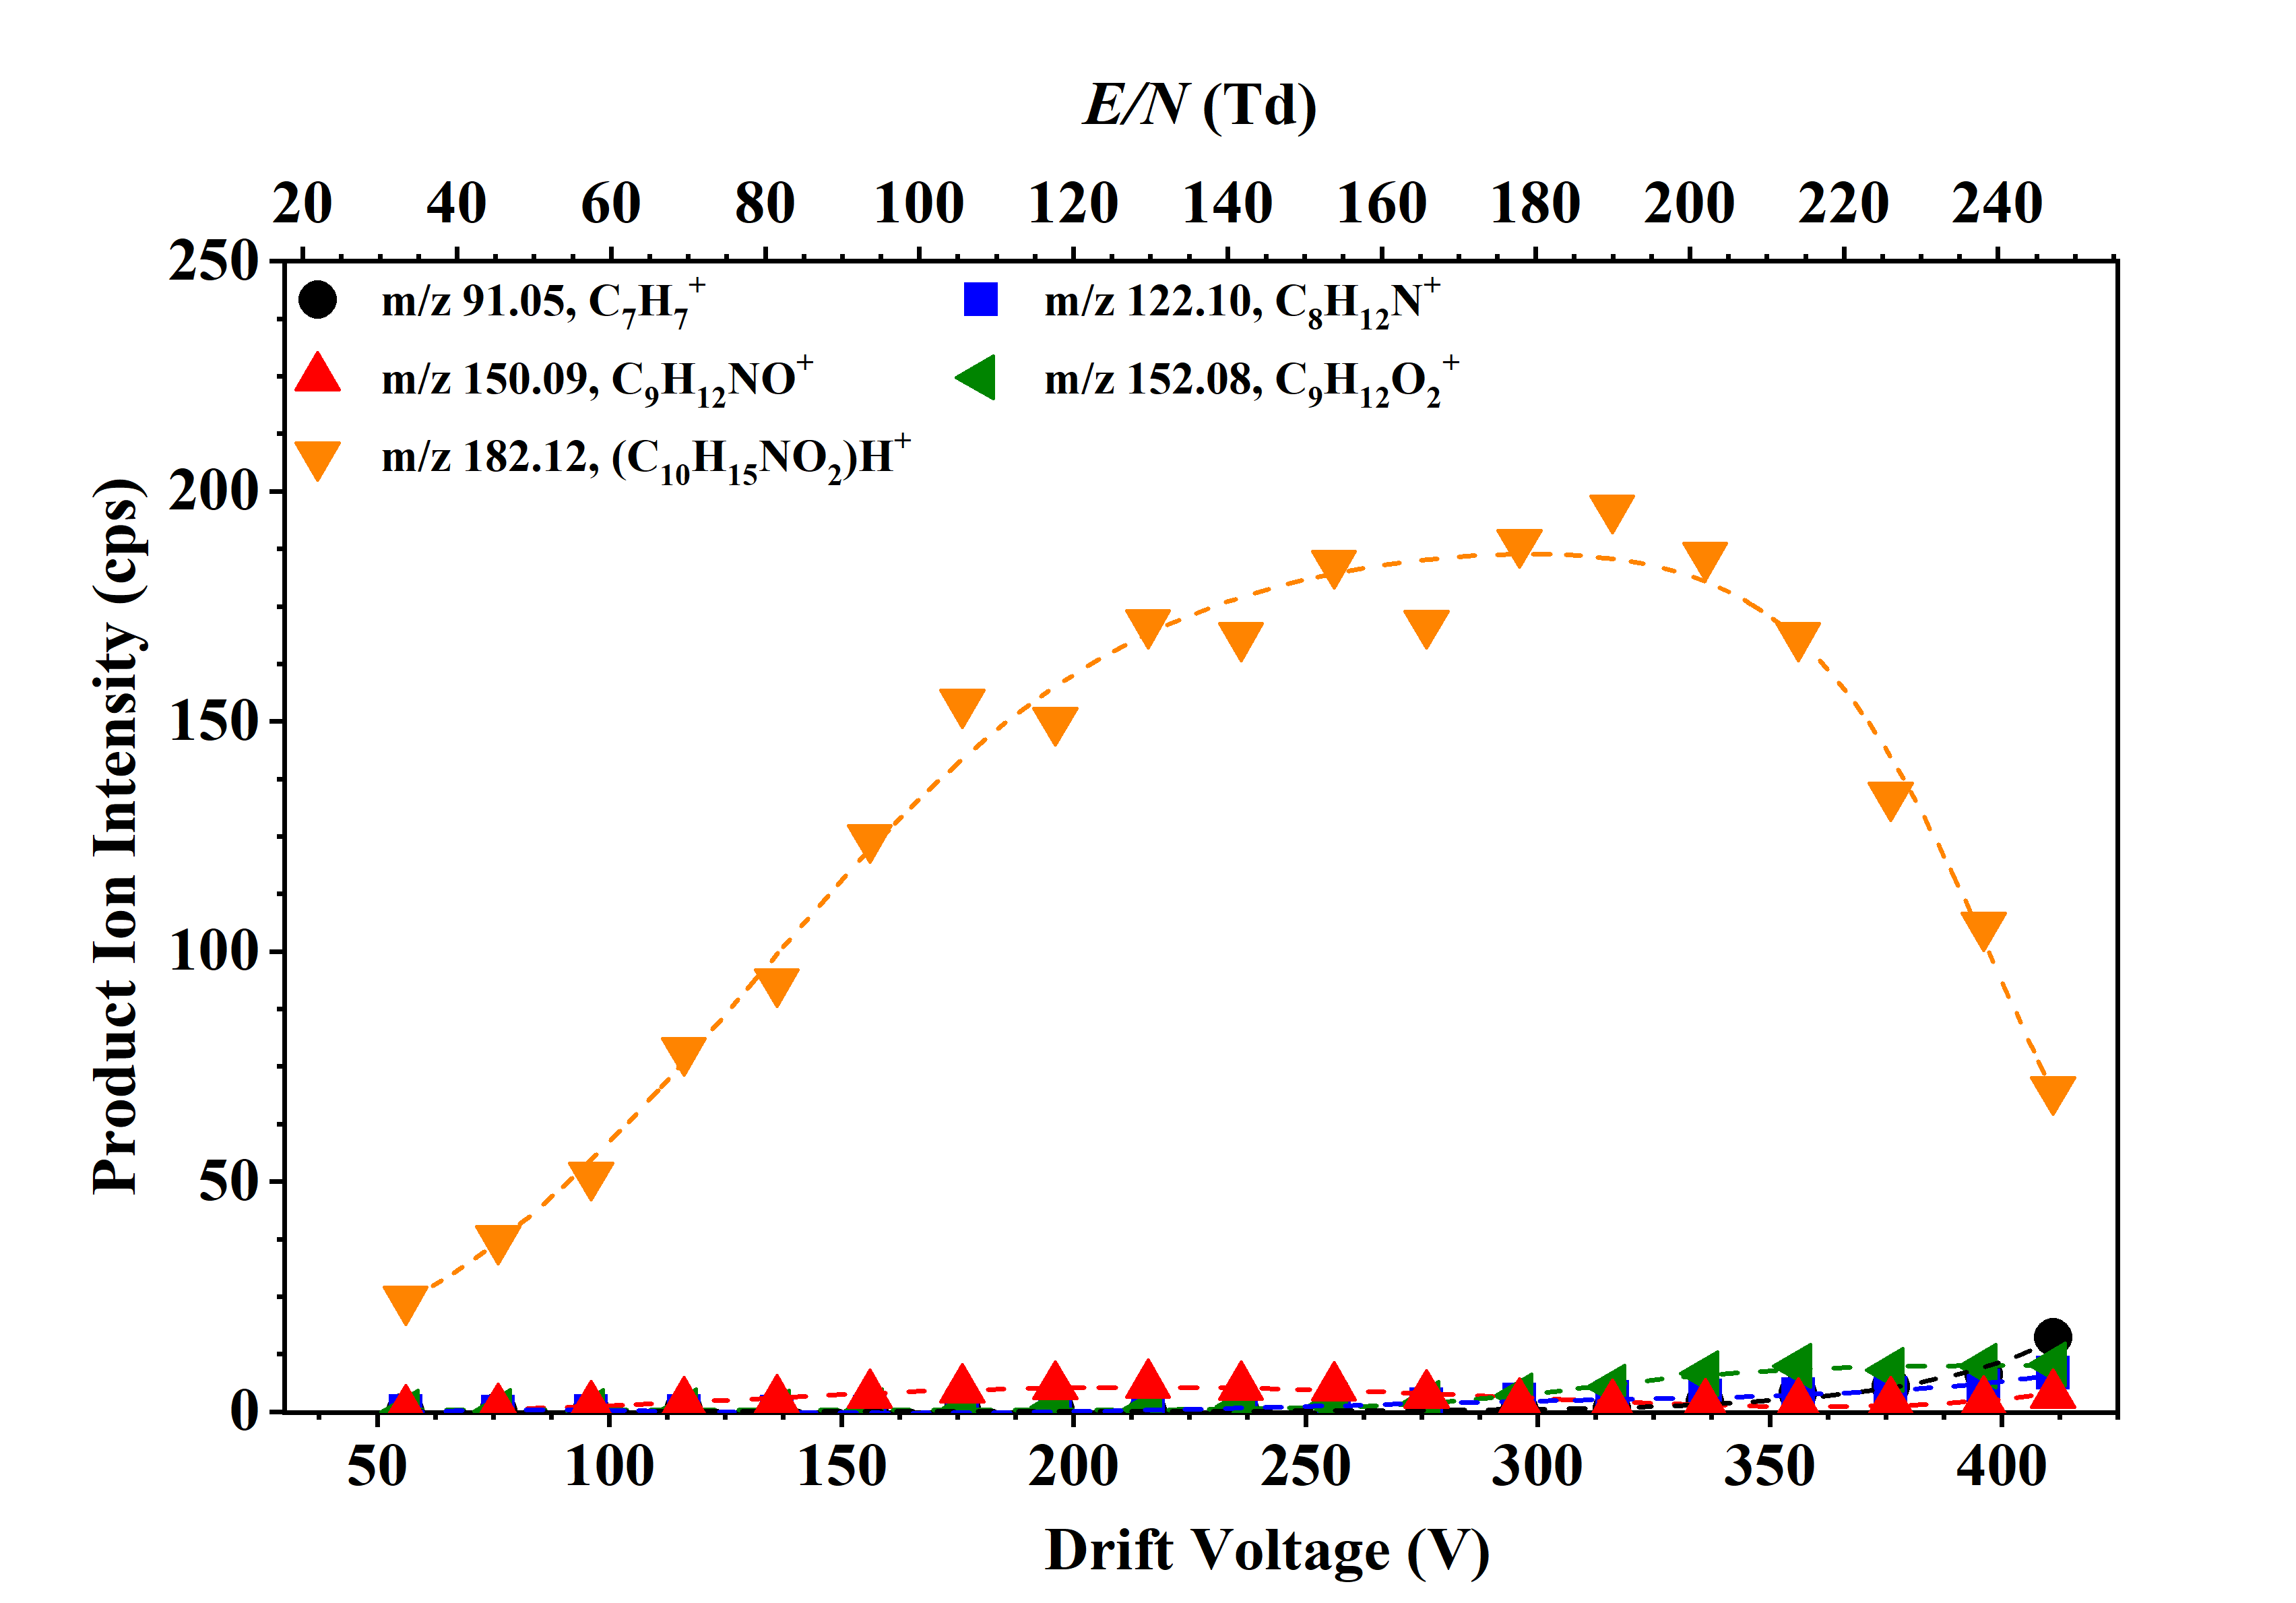
\includegraphics[width=0.8\linewidth]{pics/cocaine-chapter/ame-cps.png}
\caption{Product ion signal intensities in counts per second of the product ions resulting from reactions of the H$_3$O$^+$.(H$_2$O)$_n$ (n = 0, 1, 2) with methyl ecgonidine as a function of the drift voltage and the reduced electric field.} 
\label{fig:anhyEN}
\end{figure}


\subsection{o-Hydroxycocaine}






\begin{figure}[htbp]
\centering
\sidesubfloat[]{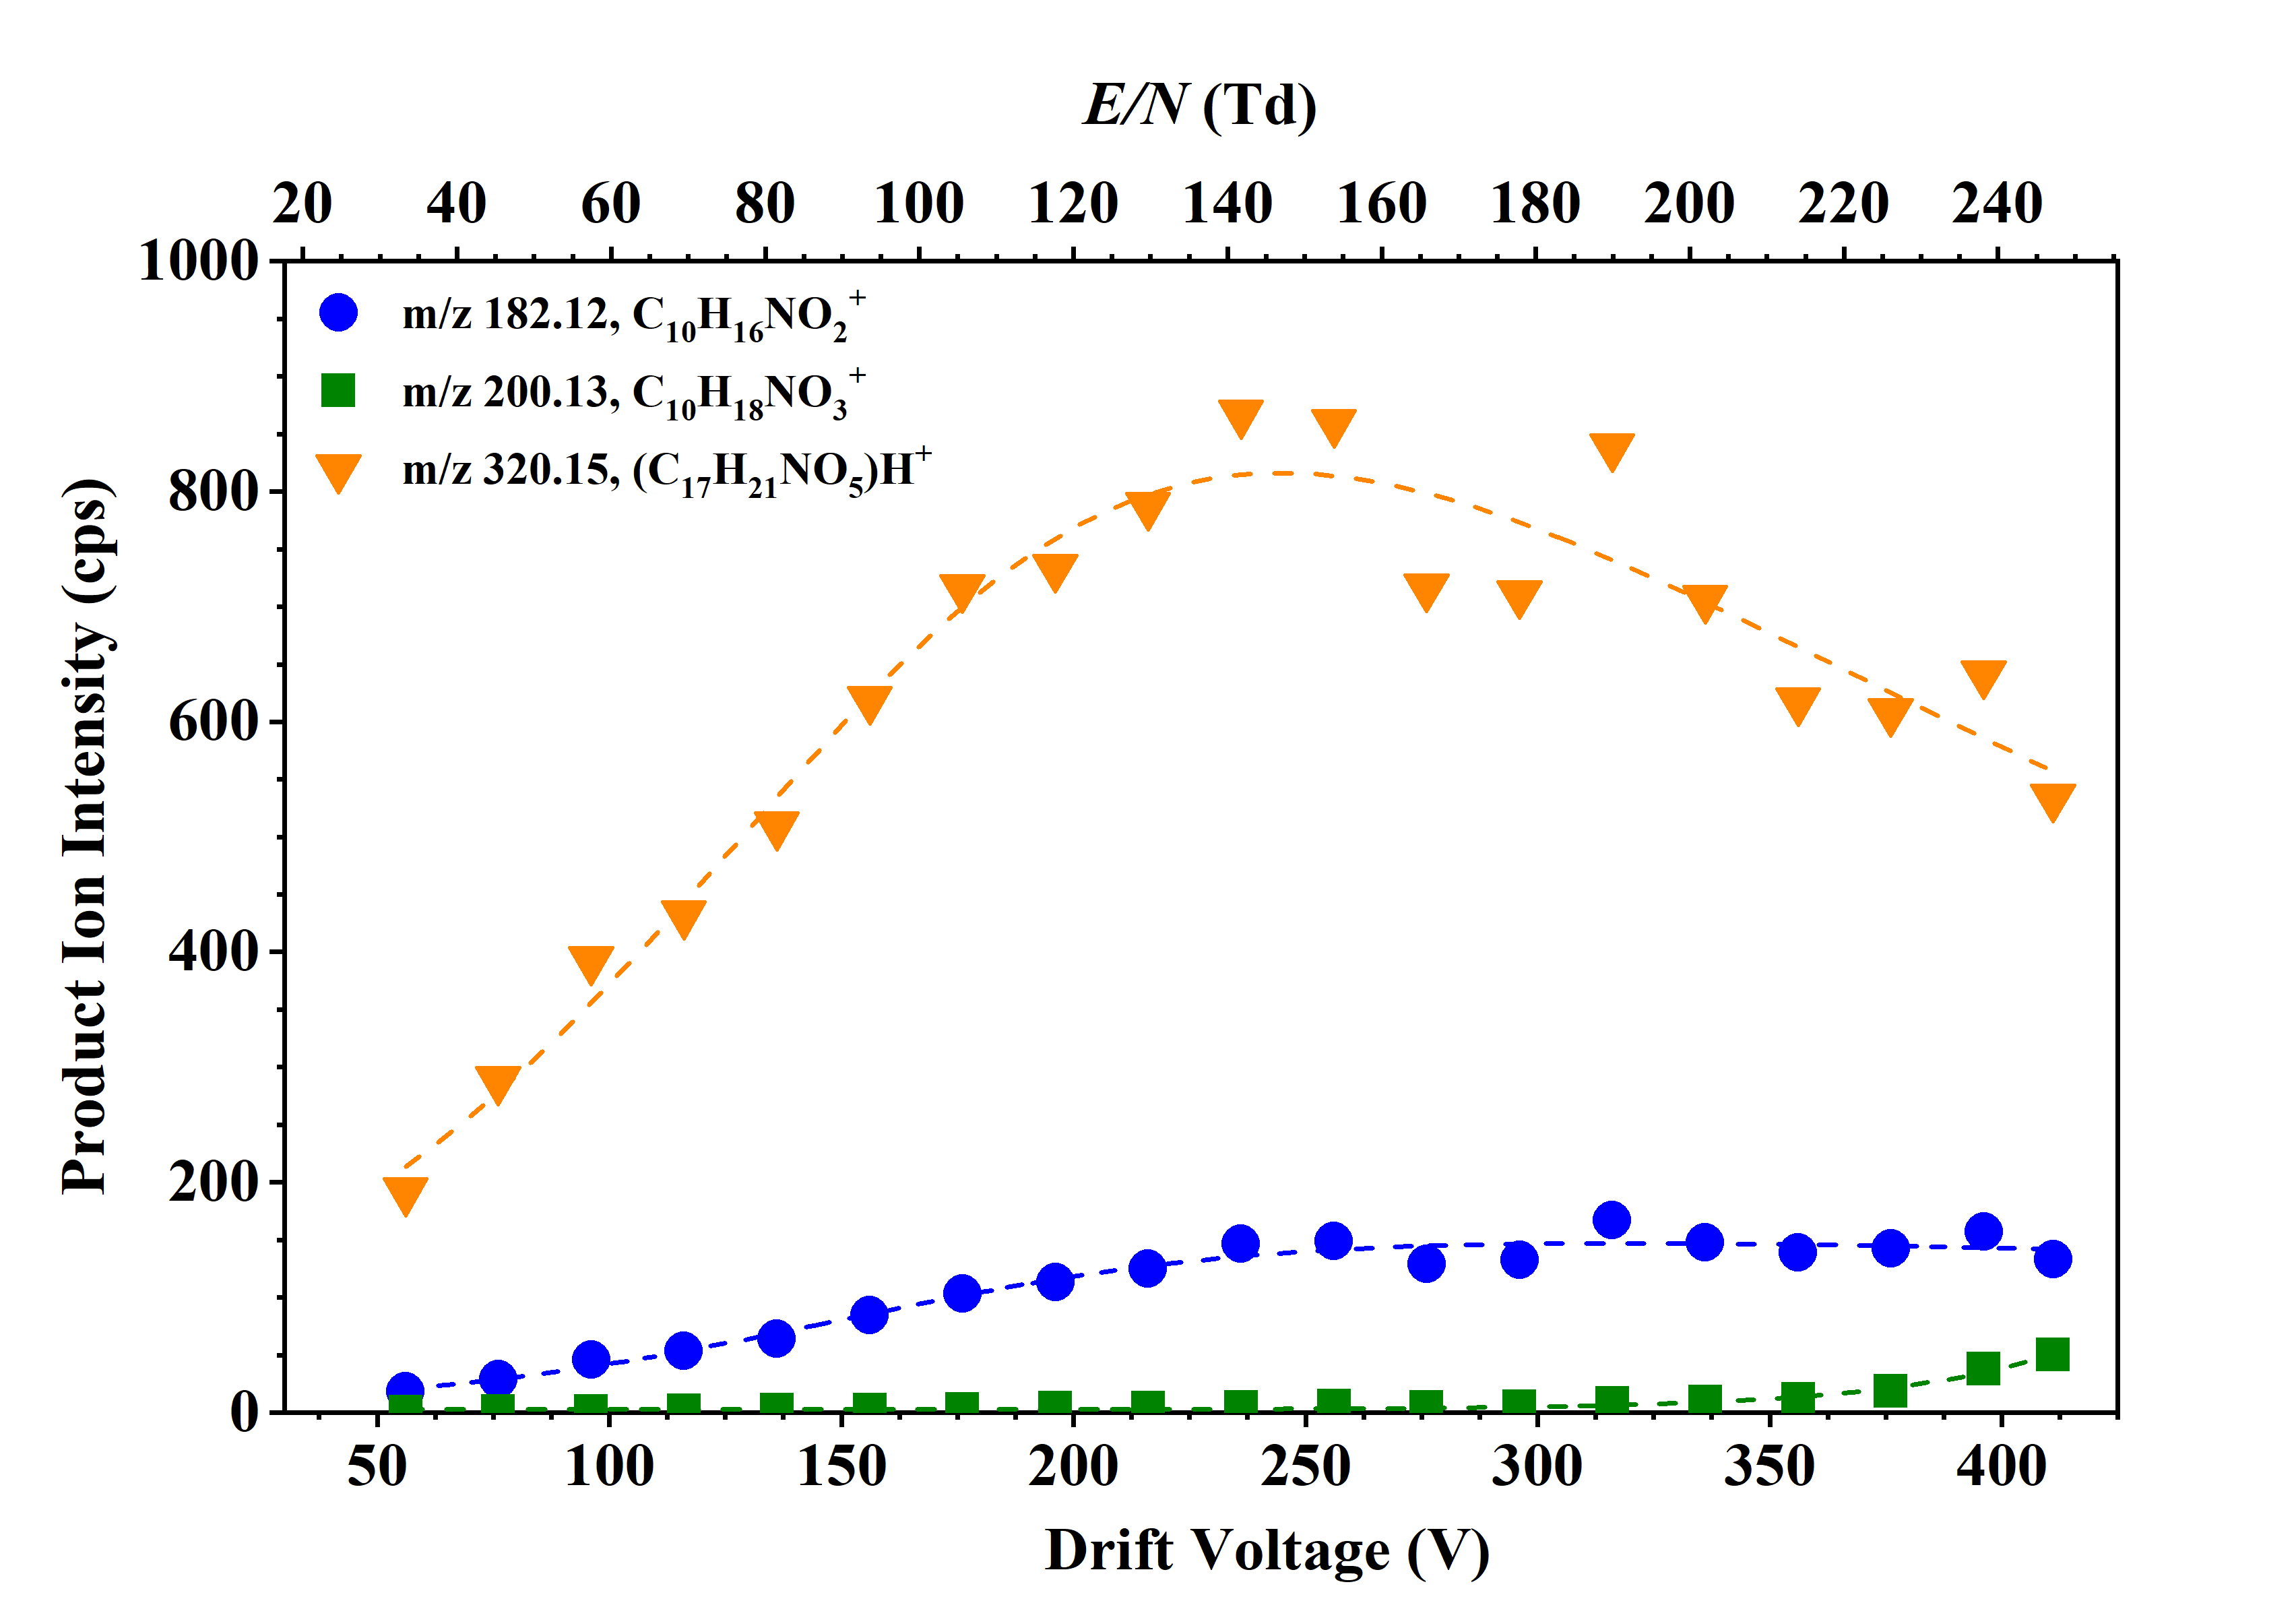
\includegraphics[width=0.8\linewidth]{pics/cocaine-chapter/ohcocaine-cps.png}}\\
\sidesubfloat[]{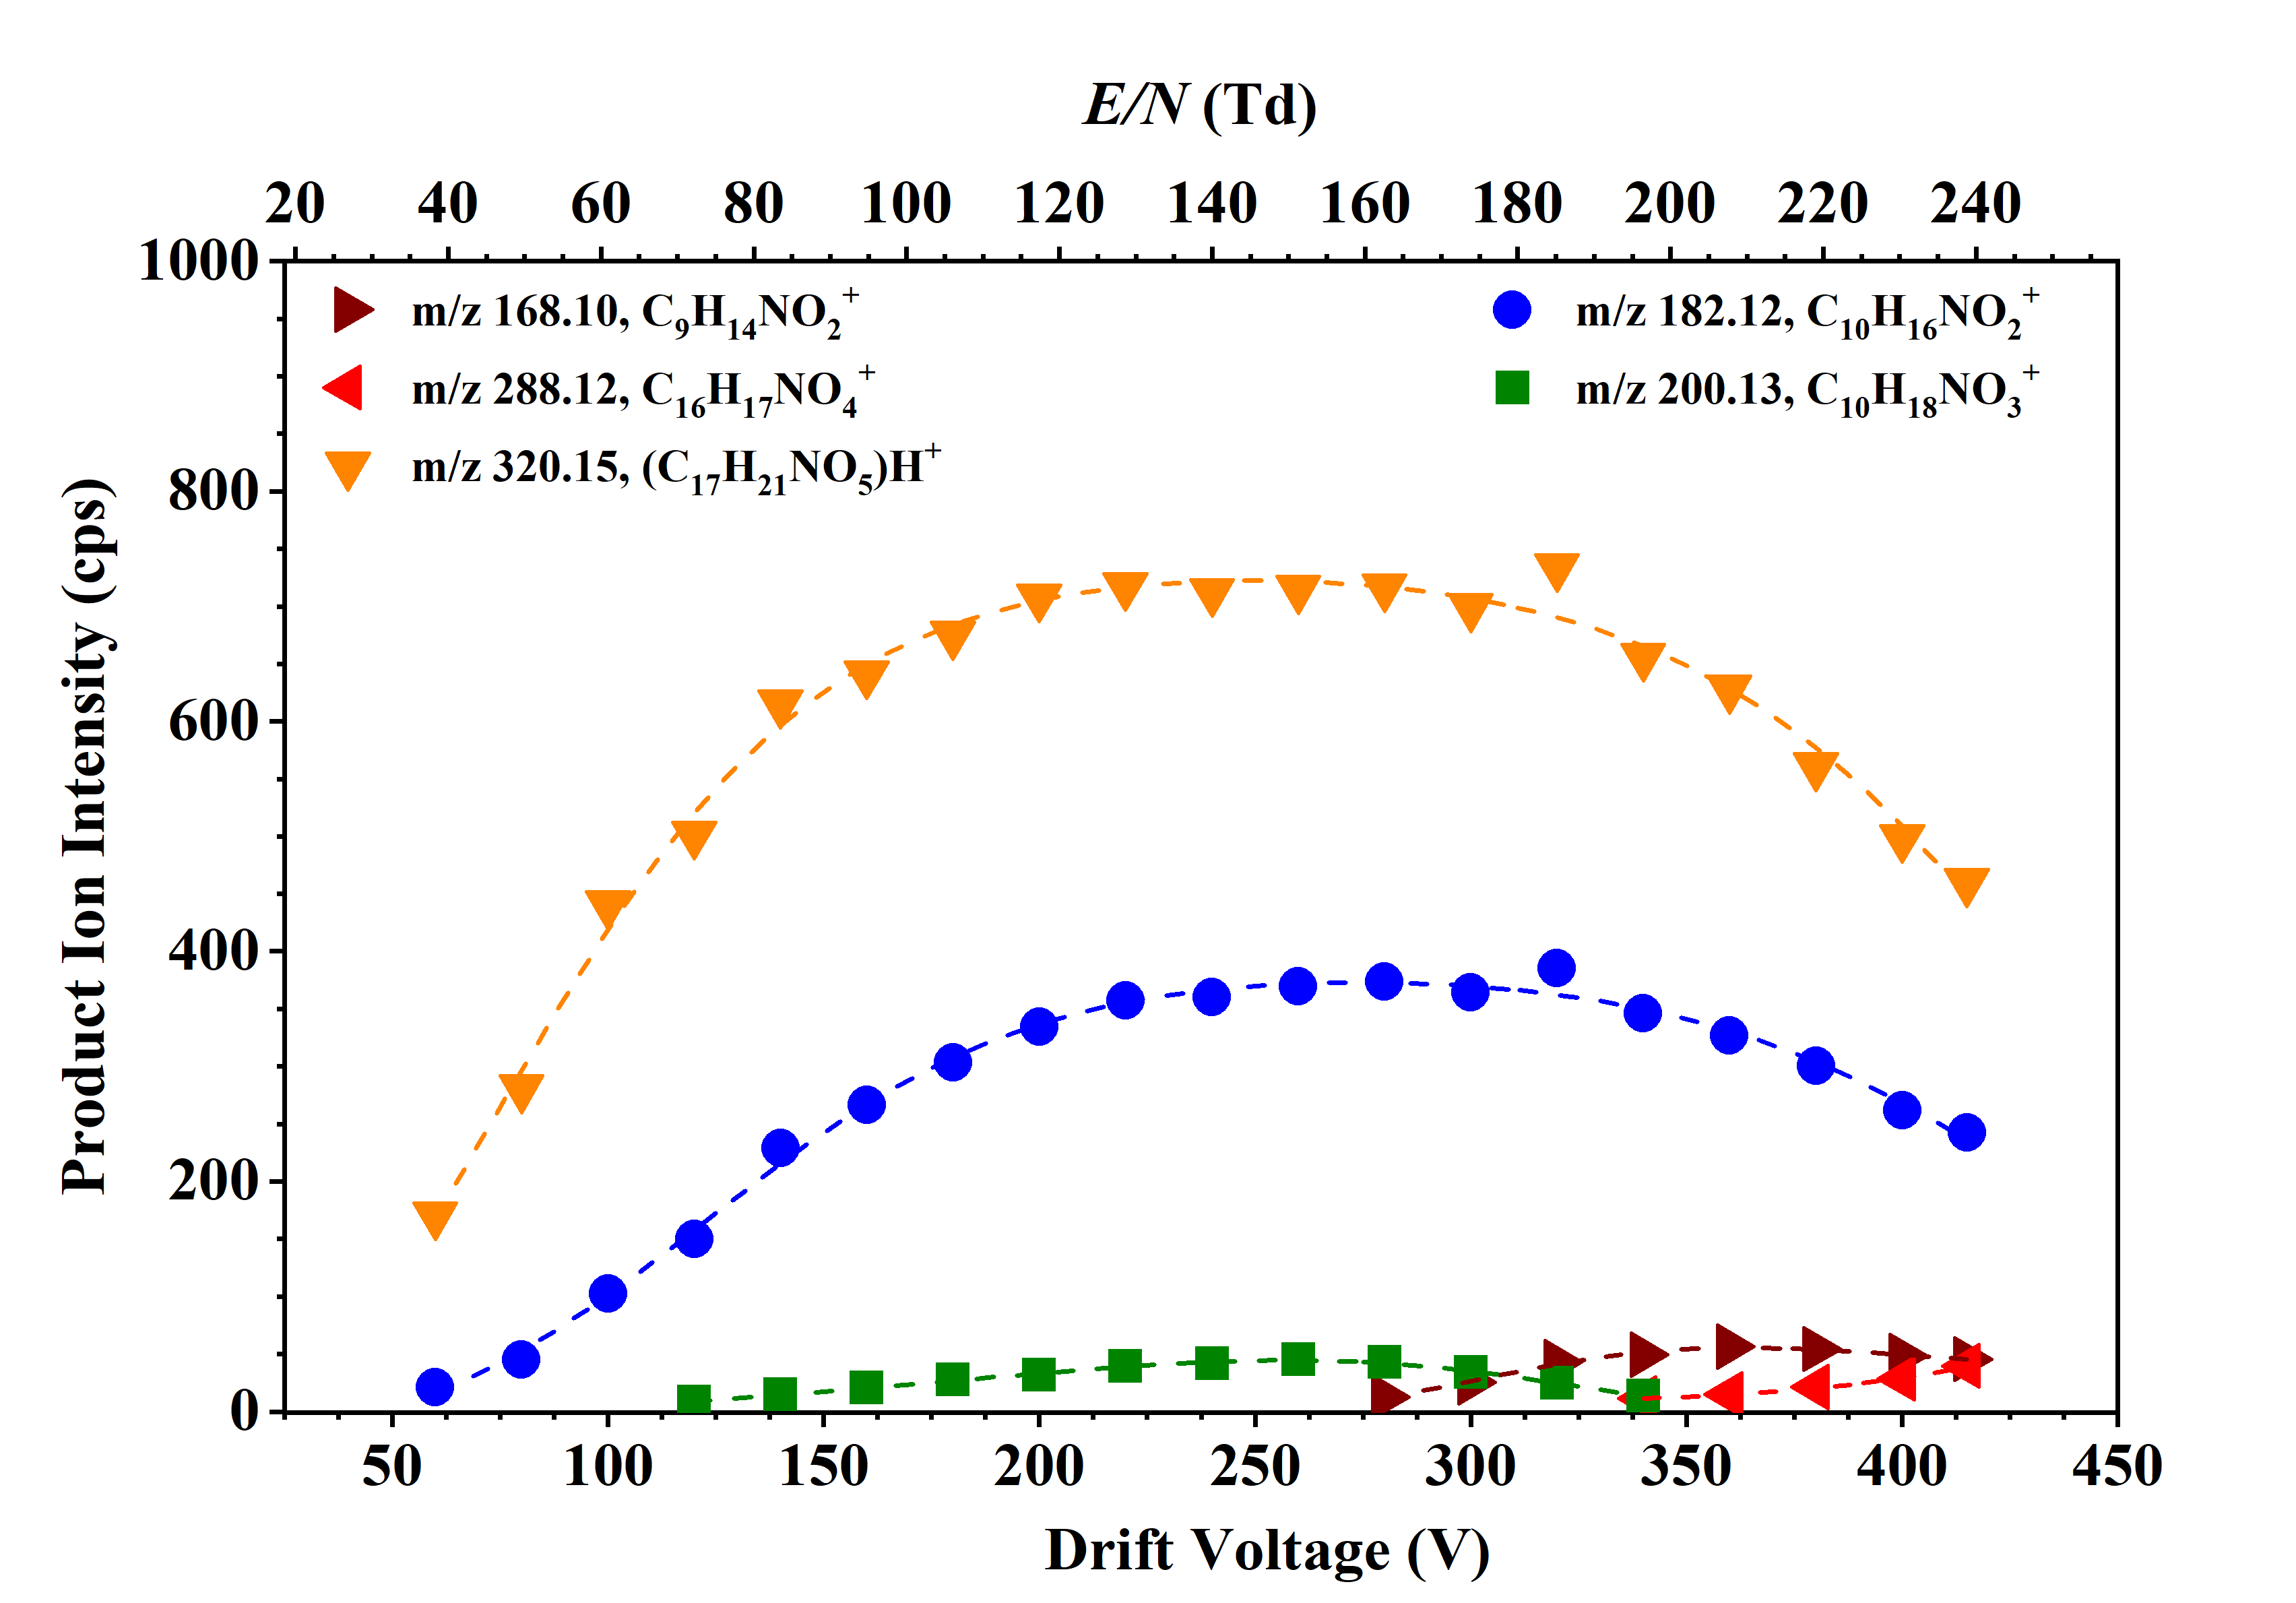
\includegraphics[width=0.8\linewidth]{pics/cocaine-chapter/humid/ohc-cps.png}}
\caption{Product ion signal intensities in counts per second of the product ions resulting from reactions of the H$_3$O$^+$.(H$_2$O)$_n$ (n = 0, 1, 2) with o-hydroxycocaine as a function of the drift voltage and the reduced electric field in (a) normal and (b) humid conditions.} 
\label{fig:ococaEN}
\end{figure}






































\section{Conclusions and further remarks}
In this chapter I have shown....

The experiments were done in two different ways....

The use of the TDU explains the dispersion of the data points for some compounds and raises concerns about the repeatability  and reproducibility, although they have been check already by \citeauthor{RN445} \cite{RN445}.


\begin{itemize}
\item For cocaine and methyl ecgonine (and ....) it is surprising that, although the proton is mobile between the various studied sites, the protonated parent molecule is the main reaction channel. 
This suggests that.... the proton stays (sequestered) in the nitrogen atom.


For many compounds (benzoates, anything else?), the MH$^+$ product ion is formed through the reactions with (H$_2$O)H$_3$O$^+$ rather than with H$_3$O$^+$, as proton transfer from the latter are dissociative. This explains in part the fact that, for the same \textit{E/N}, fragmentation is higher in the normal (dry) case.





    %\item State BzEcg difficulties. It is the main metabolite of cocaine, often measured derivatised (ref). Say that it is derivatised to be analysed. Further analysis is needed.
\end{itemize}


The loss of an alcohol (i.e. MeOH or EtOH) is a common fragmentation channel found in this chapter.
This is methanol for cocaine, while it is ethanol for cocaethylene.

DFT reveal that some fragments are not thermodynamically allowed, which hints that they are a consequence of field-activated collision-induced dissociation

The TS for the loss of benzoic acid has not been found yet. We are still looking for it.


A higher abundance of the ion at \textit{m/z} 43 for iPrBz was expected. Can this be explained in terms of the different vapour pressure of iPrBz with MeBz or EtBz????? No, because once the analyte is inside the proportions of \textit{m/z} 43 should be the same..


The most unexpected finding from the study of the isobutyrate esters is that the loss of an alcohol (i.e. MeOH for methyl isobutyrate and EtOH for ethyl isobutyrate) was only observed at high \textit{E/N}.
%
This is remarkable because the loss of an alcohol is observed in cocaine, cocaethylene, methyl ecgonine and ethyl ecgonine from low to high \textit{E/N}. 









It is also important to note that other compounds (benzoylecgonine, ecgonine and ecgonidine) that are related to cocaine presented difficulties to be measured in the same way (i.e. with the TDU). Discussions about this are still undergoing and further experiments are planned using different instrumentation.
These three compounds have a carboxylic acid group instead of the methyl or ethyl ester from the other compounds.

Benzoylecgonine is the main metabolite of cocaine. It is often measured derivatised (add ref)




















 %___________________________________________________
 %\section{OLD stuffffffffff from here on}
 
 
 

 
 
 
 
 
 
 
 
 





%\section{Results and discussion%: Measurement of illicit drugs in DC mode}}



%\subsection{Cocaethylene}










%\begin{figure}[htbp]
%\centering
%\scalebox{0.5}{
%\begin{tikzpicture}
%\chemfig{[:180]**6(------)-[::210](=[::60]O^2)-[::-60]O^4>[::75](?[a])-[::30]-[::-60,1.4](<:[::60]H)(-[::-60]N^1?[b,{-}]-[::15])-[::90,1.1]-[::135,0.8]-[::45,1.1](?[b])(<[::0]H)-[::-60]?[a](<[::45](=[::60]O^3)-[::-60]O^5-[::60]-[::-60])}
%%\chemfig{[:180]**6(------)-[::210](=[::60]O)-[::-60]O>[::75](?[a])-[::30]-[::-60,1.4](<:[::60]H)(-[::120]N?[b,{-}]-[::-15])-[::-30,1.1]-[::-90,0.8]-[::-90,1.1](?[b])(<[::105]H)-[::60]?[a](<[::45](=[::60]O)-[::-60]O-[::60])} %previous version with the N in opposite way
%\end{tikzpicture}
%}\label{fig:cocet}
%\caption{Cocaethylene}
%\end{figure}


%\subsection{Ethyl ecgonine}








%\begin{figure}[htbp]
%\centering
%\scalebox{0.5}{
%\begin{tikzpicture}
%\chemfig{[:-30]O^4(-[::180]H)>[::60](?[a])-[::45]-[::-60,1.4](<:[::60]H)(-[::-60]N^1?[b,{-}]-[::15])-[::90,1.1]-[::135,0.8]-[::45,1.1](?[b])(<[::0]H)-[::-60]?[a](<[::45](=[::60]O^3)-[::-60]O^5-[::60]-[::-60])}
%\end{tikzpicture}
%}\label{fig:etecg}
%\caption{Ethyl ecgonine}
%\end{figure}












%\subsection{Ecgonine}







%\begin{figure}[htbp]
%\centering
%\scalebox{0.5}{
%\begin{tikzpicture}
%\chemfig{[:-30]O^4(-[::180]H)>[::75](?[a])-[::30]-[::-60,1.4](<:[::60]H)(-[::-60]N^1?[b,{-}]-[::15])-[::90,1.1]-[::135,0.8]-[::45,1.1](?[b])(<[::0]H)-[::-60]?[a](<[::45](=[::60]O^3)-[::-60]O^5-[::60]H)}
%\end{tikzpicture}}
%\caption{Ecgonine}\label{fig:ecgonine}
%\end{figure}





%\subsection{Ecgonidine}



%\begin{figure}[htbp]
%\centering
%\scalebox{0.5}{
%\begin{tikzpicture}
%\chemfig{[:30](?[a])-[::45]-[::-60,1.4](<:[::60]H)(-[::-60]N?[b,{-}]-[::15])-[::90,1.1]-[::135,0.8]-[::45,1.1](?[b])(<[::0]H)-[::-60]?[a,{=}](<[::45](=[::60]O)-[::-60]O-[::60]H)}
%\end{tikzpicture}}
%\caption{Ecgonidine}\label{fig:ed}
%\end{figure}












%\subsection{Methyl ecgonidine}


%\begin{figure}
%\begin{center}
%\begin{tikzpicture}[scale=1.0]
%\tikzstyle{every node}=[font=\small]
%\begin{axis}[clip=false,ylabel=$\Delta$G (kJ/mol),xlabel=Reaction coordinate,xtick=\empty,legend pos=outer north east,xmin=0.5,xmax=14,ymax=120,ymin=-220,axis lines = left]
%\addplot[color=black,draw=blue,line width=1pt] coordinates {(2,0)(3,0)};
%\addplot[color=black,line width=0.8pt,densely dotted] coordinates {(3,0)(4,-178)};
%\addplot[color=black,draw=blue,line width=1pt] coordinates {(4,-178)(5,-178)};
%\addplot[color=black,line width=0.8pt,densely dotted] coordinates {(5,-178)(6,-41)};
%\addplot[color=black,draw=blue,line width=1pt] coordinates {(6,-41)(7,-41)};
%\addplot[color=black,line width=0.8pt,densely dotted] coordinates {(7,-41)(8,-120)};
%\addplot[color=black,draw=blue,line width=1pt] coordinates {(8,-120)(9,-120)};
%\addplot[color=black,line width=0.8pt,densely dotted] coordinates {(9,-120)(10,71)};
%\addplot[color=black,draw=blue,line width=1pt] coordinates {(10,71)(11,71)};
%\addplot[color=black,line width=0.8pt,densely dotted] coordinates {(11,71)(12,-77)};
%\addplot[color=black,draw=blue,line width=1pt] coordinates {(12,-77)(13,-77)};
%\node [text width=2cm] at (axis cs:2.5,20) {EtBz + H$_3$O$^+$};
%\node [text width=2cm] at (axis cs:4.5,-200) {EtBz1H$^+$};
%\node [text width=3cm] at (axis cs:6.5,-20) {TS for loss of C$_2$H$_4$};
%\node [text width=3cm] at (axis cs:8.5,-140) {BzAcidH$^+$ + C$_2$H$_4$};
%\node [text width=3cm] at (axis cs:10.5,90) {TS for loss of H$_2$O to Benzoyl$^+$};
%\node [text width=3cm] at (axis cs:12.5,-97) {Benzoyl$^+$ + C$_2$H$_4$};
%\node at (2.5,3) {\includegraphics[scale=0.1]{rea1.pdf}};
%\node at (axis cs:2.1,-10) {\includegraphics[scale=0.06,angle=90]{r1.pdf}};
%\node at (axis cs:3.2,-10) {\includegraphics[scale=0.06,angle=90]{r2.pdf}};
%\node at (axis cs:4.3,50) {\includegraphics[scale=0.08,angle=90]{t1.pdf}};
%\node at (axis cs:6.9,-35) {\includegraphics[scale=0.08,angle=90]{p1.pdf}};
%\end{axis}
%\end{tikzpicture}
%\end{center}
%\caption{$\Delta$G for reaction of H$_3$O$^+$ with EtBz –- Example of the data from Peter Watts}\label{fig:trans.example}
%\end{figure}




%\begin{figure}[htbp]
%\begin{center}
%\schemedebug{false}
%\schemestart[0,1,thick]
%\chemname{\scalebox{0.4}{\chemfig{**6(----(-[::-60](=[::60]O^1)-[::-60]O^2(-[::60]-[::-60]))--)}}\+\chemfig{H_3O^+}}{Ethyl benzoate}
%\arrow(nph.south--aa7)[-150,2]
%		\chemname{\scalebox{0.4}{\chemfig{**6(----(-[::-60](-[,0.2,,,draw=none]\+)(-[::60]O-[::-60]H)-[::-60]O(-[::60]-[::-60]))--)}}}{Ethyl benzoate 1H$^+$}
%	\arrow[-90]
%		\chemname{\scalebox{0.4}{\chemfig{**6(----(-[::-60](-[,0.2,,,draw=none]\+)(-[::60]O-[::-60]H)-[::-60]O(-[@{db}::-30]-[@{a1}::90]-[@{db2}::90]H-[@{a2}::90,,,,draw=none]))--)}
%    	\chemmove{\draw(db)..controls +(120:4mm) and +(150:4mm)..(a1);
%    	\draw(db2)..controls +(-60:4mm) and +(-30:4mm)..(a2);}}%\+\chemfig{H_2O}                }{TS1 from 1H$^+$}
%	\arrow(aa11--ba)[-90]
%    	\chemname{\scalebox{0.4}{\chemfig{**6(----(-[::-60](-[,0.2,,,draw=none]\+)(-[::60]O-[::-60]H)-[::-60]O(-[::60]H))--)}}}{BzAcidH$^+$}
%	\arrow(@ba--)[-90]
%    	\chemname{\scalebox{0.4}{\chemfig{**6(----(-[::-60](-[,0.2,,,draw=none]\+)(-[@{a3}::60]O-[@{db3}::-60]H-[@{a4}::-120,1.5,,,draw=none])-[@{db4}::-60]O(-[::60]H))--)}
%        \chemmove{\draw(db3)..controls +(0:4mm) and +(90:4mm)..(a3);
%    	\draw(db4)..controls +(270:4mm) and +(270:4mm)..(a4);}        }}{TS3 (loss of water)}
%	\arrow(aa10--aa2)[0,3.7]
%    	\chemname{\scalebox{0.4}{\chemfig{**6(----(-[::-60](-[,0.2,,,draw=none]\+)=[::60]O)--)}}}{Benzoyl$^+$}
%\arrow(@nph.south--aa3)[-30,2]
%		\chemname{\scalebox{0.4}{\chemfig{**6(----(-[::-60](=[::60]O)-[::-60]O^+(-[::-60]H)(-[::60]-[::-60]))--)}}}{Ethyl benzoate 2H$^+$}
%	\arrow(.south--aa4)[-135,2.5]
%    	\chemname{\scalebox{0.4}{\chemfig{**6(----(-[::-60](*6(-O^+(-[::-60]H)-[@{db6}]-[@{a6}]-H-[@{a5},,,,draw=none]O=[@{db5}])))--)}
%		\chemmove{\draw(db5)..controls +(60:4mm) and +(0:4mm)..(a5);
 %   	\draw(db6)..controls +(180:4mm) and +(240:4mm)..(a6);}		}}{TS2 from 2H$^+$}
%     \arrow(@aa3.south--@aa2)
%    \arrow(@aa4.mid west--@ba)
%    \arrow(@aa7--aa8.)[0,1.3]
%        	\chemname{\scalebox{0.4}{\chemfig{**6(----(-[::-60](*6(-O^+(-[@{db6}::-60,,,,draw=none])-(-[::-60])-[,,,,draw=none]-[,,,,draw=none]H(-[@{a6}::-240,,,,draw=none])-[@{a5}]O-[@{db5}])))--)}
%		\chemmove{\draw(a5)..controls +(0:4mm) and +(60:4mm)..(db5);
%		\draw(db6)..controls +(-120:10mm) and +(-90:10mm)..(a6);}		}}{TS from 1H$^+$ to 2H$^+$}
%		\arrow(.east--aa3)[0,1.3]
%\schemestop
%\end{center}
%\caption{Ethyl benzoate}\label{fig:eb1}
%\end{figure}









































%\subsection{Characterisation of the TDU: temperature study}

%\subsubsection{HMTD}
%Using ------------------- as probe I have done a temperature study of the TDU keeping the rest of the temperatures and pressures constant.

%Use HMTD for this (I can't put this in my thesis as it is in a paper already. put reference to the paper)   

%\textbf{use the counts per second!!! It is what makes sense}

%I measured at different TDU temperatures: 100$^{\circ}$C, 150$^{\circ}$C and 200$^{\circ}$C, while keeping the inlet line and the oven at 150$^{\circ}$C, so the differences come purely from the TDU temperature


%\begin{figure}
%\scalebox{0.7}{\begin{tikzpicture}\chemfig{N(-[::90,,,,line width=3pt]>[::-30]O-[::-30]O-[::-45]-[::-75]N?[b])(-[::-30,,,,line width=3pt]>[::30]O-[::30]O-[::30]?[b])(-[::-150,,,,line width=3pt]>[::-135]O-[::-45]O-[::-30]?[b])
%}\end{tikzpicture}}
%\caption{Structure of HMTD.}\label{fig:hmtd}
%\end{figure}

%\subsubsection{Benzoylecgonine}
%Add measurements from 31st October 2018 (latex report)











